\chapter{Right Triangle Trigonometry}
Trigonometry is the study of the relations between the sides and angles of triangles. The word
``trigonometry'' is derived from the Greek words \emph{trigono}
($\othertau\otherrho\acute{\otheriota}\othergamma\otheromega\othernu$o), meaning ``triangle'', and \emph{metro}
($\othermu\otherepsilon\othertau\otherrho\acute{\otheromega}$), meaning ``measure''. Though the ancient Greeks,
such as Hipparchus\index{Hipparchus} and Ptolemy\index{Ptolemy}, used trigonometry in their study of
astronomy between roughly 150 \textsc{b.c.} - \textsc{a.d.} 200, its history is much older.
For example, the Egyptian scribe Ahmes\index{Ahmes} recorded some rudimentary
trigonometric calculations (concerning ratios of sides of pyramids) in the famous Rhind
Papyrus\index{Rhind Papyrus} sometime around 1650 \textsc{b.c.}\footnote{Ahmes claimed that he
copied the papyrus from a work that may date as far back as 3000 \textsc{b.c.}}

Trigonometry is distinguished from elementary geometry in part by its extensive use of certain
functions of angles, known as the \emph{trigonometric functions}. Before discussing those functions,
we will review some basic terminology about angles.

%Begin Section 1.1
\section{Angles}
Recall the following definitions from elementary geometry:\index{angle}
\begin{enumerate}[\bfseries (a)]
 \item An angle is \textbf{acute}\index{acute angle}\index{angle!acute} if it is between $0\Degrees$
  and $90\Degrees$.
 \item An angle is a \textbf{right angle}\index{right angle}\index{angle!right} if it equals
  $90\Degrees$.
 \item An angle is \textbf{obtuse}\index{obtuse angle}\index{angle!obtuse} if it is between
  $90\Degrees$ and $180\Degrees$.
 \item An angle is a \textbf{straight angle}\index{straight angle}\index{angle!straight} if it
  equals $180\Degrees$.
\end{enumerate}

\begin{figure}[h]
 \centering
 \subfloat[][ acute angle]{
 \begin{tikzpicture}
  \draw [line width=0.5pt,-latex] (0.7,0) arc (0:45:0.7);
  \draw [linecolor,line width=1.5pt,latex-latex] (1.5,0) -- (0,0) -- (1.3,1.3);
  \draw [white] (1.6,0) -- (2.1,0);
  \draw [white] (-0.1,0) -- (-0.5,0);
 \end{tikzpicture}}
 \qquad
 \subfloat[][ right angle]{
 \begin{tikzpicture}
  \draw [line width=0.5pt,-latex] (0.7,0) arc (0:90:0.7);
  \draw [line width=0.5pt] (0.2,0) -- (0.2,0.2) -- (0,0.2);
  \draw [linecolor,line width=1.5pt,latex-latex] (1.5,0) -- (0,0) -- (0,1.3);
  \draw [white] (1.6,0) -- (2.1,0);
  \draw [white] (-0.1,0) -- (-0.5,0);
 \end{tikzpicture}}
 \qquad
 \subfloat[][ obtuse angle]{
 \begin{tikzpicture}
  \draw [line width=0.5pt,-latex] (0.7,0) arc (0:135:0.7);
  \draw [linecolor,line width=1.5pt,latex-latex] (1.5,0) -- (0,0) -- (-1.3,1.3);
 \end{tikzpicture}}
 \qquad
 \subfloat[][ straight angle]{
 \begin{tikzpicture}
  \draw [line width=0.5pt,-latex] (0.7,0) arc (0:180:0.7);
  \draw [linecolor,line width=1.5pt,latex-latex] (-1.5,0) -- (0,0) -- (1.5,0);
 \end{tikzpicture}}
 \caption[]{\quad Types of angles}
 \label{fig:angles}
\end{figure}

In elementary geometry, angles are always considered to be positive and not larger than
$360\Degrees$. For now we will only consider such angles.\footnote{Later in the text we will
discuss negative angles and angles larger than $360\Degrees$.} The following definitions will be
used throughout the text:
\newpage
\begin{enumerate}[\bfseries (a)]
 \item Two acute angles are \textbf{complementary}\index{complementary angles} if their sum equals
  $90\Degrees$. In other words, if $0\Degrees \le \angle\,A \,,\, \angle\,B \le 90\Degrees$ then
  $\angle\,A$ and $\angle\,B$ are complementary if $\angle\,A + \angle\,B = 90\Degrees$.
 \item Two angles between $0\Degrees$ and $180\Degrees$ are
  \textbf{supplementary}\index{supplementary angles} if their sum equals $180\Degrees$. In other
  words, if $0\Degrees \le \angle\,A \,,\, \angle\,B \le 180\Degrees$ then $\angle\,A$ and
  $\angle\,B$ are supplementary if $\angle\,A + \angle\,B = 180\Degrees$.
 \item Two angles between $0\Degrees$ and $360\Degrees$ are \textbf{conjugate}\index{conjugate
  angles} (or \textbf{explementary}\index{explementary angles}) if their sum equals $360\Degrees$.
  In other words, if $0\Degrees \le \angle\,A \,,\, \angle\,B
  \le 360\Degrees$ then $\angle\,A$ and $\angle\,B$ are conjugate if $\angle\,A + \angle\,B =
  360\Degrees$.
\end{enumerate}

\begin{figure}[h]
 \centering
 \subfloat[][ complementary]{
 \begin{tikzpicture}
  \draw [line width=0.5pt,latex-] (0,1) arc (90:56.3:1);
  \draw [line width=0.5pt,-latex] (1,0) arc (0:56.3:1);
  \draw [line width=0.5pt] (0.2,0) -- (0.2,0.2) -- (0,0.2);
  \draw [linecolor,line width=1.5pt,latex-latex] (1.5,0) -- (0,0) -- (0,1.8);
  \draw [linecolor,line width=1.5pt,-latex] (0,0) -- (1,1.5);
  \draw [white] (1.6,0) -- (2.3,0);
  \draw [white] (-0.1,0) -- (-0.7,0);
  \node [right] at (0.85,0.6) {\small $\angle\,A$};
  \node [above] at (0.35,1) {\small $\angle\,B$};
 \end{tikzpicture}}
 \qquad\qquad
 \subfloat[][ supplementary]{
 \begin{tikzpicture}
  \draw [line width=0.5pt,-latex] (0.7,0) arc (0:135:0.7);
  \draw [line width=0.5pt,latex-] (-0.7,0) arc (180:135:0.7);
  \draw [linecolor,line width=1.5pt,latex-latex] (-1.8,0) -- (1.8,0);
  \draw [linecolor,line width=1.5pt,-latex] (0,0) -- (-1.3,1.3);
  \node [above right] at (0.1,0.8) {\small $\angle\,A$};
  \node [above left] at (-0.65,0.25) {\small $\angle\,B$};
 \end{tikzpicture}}
 \qquad\qquad
 \subfloat[][ conjugate]{
 \begin{tikzpicture}
  \draw [line width=0.5pt,latex-] (0.7,0) arc (360:56.3:0.7);
  \draw [line width=0.5pt,-latex] (0.7,0) arc (0:56.3:0.7);
  \draw [linecolor,line width=1.5pt,latex-latex] (1.5,0) -- (0,0) -- (1,1.5);
  \node [right] at (0.8,0.5) {\small $\angle\,A$};
  \node [above] at (-0.7,0.5) {\small $\angle\,B$};
 \end{tikzpicture}}
 \caption[]{\quad Types of pairs of angles}
 \label{fig:angles2}
\end{figure}\vspace{-2mm}

Instead of using the angle notation $\angle\,A$ to denote an angle, we will sometimes use just a
capital letter by itself (e.g. $A$, $B$, $C$) or a lowercase variable name (e.g. $x$, $y$, $t$).
It is also common to use letters (either uppercase or lowercase) from the Greek alphabet, shown
in the table below, to represent angles:\index{Greek alphabet}\vspace{-3mm}

\begin{table}[h]\centering
\caption{\quad \textbf{The Greek alphabet}}\vspace{3mm}
\begin{tabular}{lll!{\qquad\qquad}lll!{\qquad\qquad}lll}
\hline\\[0.5pt]
\multicolumn{2}{l}{\textbf{Letters}} & \textbf{Name} & \multicolumn{2}{l}{\textbf{Letters}} &
 \textbf{Name} & \multicolumn{2}{l}{\textbf{Letters}} & \textbf{Name}\\[4pt]
A & $\alpha$ & alpha & I & $\iota$ & iota & P & $\rho$ & rho\\
B & $\beta$ & beta & K & $\kappa$ & kappa & $\Sigma$ & $\sigma$ & sigma\\
$\Gamma$ & $\gamma$ & gamma & $\Lambda$ & $\lambda$ & lambda & T & $\tau$ & tau\\
$\Delta$ & $\delta$ & delta & M & $\mu$ & mu & $\Upsilon$ & $\upsilon$ & upsilon\\
E & $\epsilon$ & epsilon & N & $\nu$ & nu & $\Phi$ & $\phi$ & phi\\
Z & $\zeta$ & zeta & $\Xi$ & $\xi$ & xi & X & $\chi$ & chi\\
H & $\eta$ & eta & O & $o$ & omicron & $\Psi$ & $\psi$ & psi\\
$\Theta$ & $\theta$ & theta & $\Pi$ & $\pi$ & pi & $\Omega$ & $\omega$ & omega\\[1pt]\\
\hline
\end{tabular}
\end{table}

In elementary geometry you learned that the sum of the angles in a triangle equals $180\Degrees$,
and that an \textbf{isosceles triangle}\index{isosceles triangle}\index{triangle!isosceles} is a
triangle with two sides of equal length.
Recall that in a \textbf{right triangle}\index{right triangle}\index{triangle!right} one of the
angles is a right angle. Thus, in a right triangle\index{triangle} one of the angles is
$90\Degrees$ and the other two angles are acute angles whose sum is $90\Degrees$ (i.e. the other two
angles are complementary angles).
\newpage
\begin{exmp}
 For each triangle below, determine the unknown angle(s):
  \begin{center}
  \begin{tikzpicture}
   \filldraw [linecolor,line width=1.5pt,fill=fillcolor] (0,0) -- (4,0) -- (35:1.7) -- cycle;
   \node [below left] at (0,0) {\small $A$};
   \node [above] at (35:1.7) {\small $B$};
   \node [below right] at (4,0) {\small $C$};
   \node at (15:0.75) {\small $35\Degrees$};
   \node at (2.8,0.2) {\small $20\Degrees$};

   \filldraw [linecolor,line width=1.5pt,fill=fillcolor] (6,0) -- (8,0) -- (8,1.5) -- cycle;
   \draw (7.8,0.025) -- (7.8,0.23) -- (7.975,0.23);
   \node [below left] at (6,0) {\small $D$};
   \node [above right] at (8,1.5) {\small $E$};
   \node [below right] at (8,0) {\small $F$};
   \node at (7.7,0.9) {\small $53\Degrees$};

   \filldraw [linecolor,line width=1.5pt,fill=fillcolor] (10,0) -- (13,0) -- (11.5,1.3) -- cycle;
   \node [below left] at (10,0) {\small $X$};
   \node [above] at (11.5,1.3) {\small $Y$};
   \node [below right] at (13,0) {\small $Z$};
   \node at (10.5,0.2) {\small $\alpha$};
   \node at (12.5,0.2) {\small $\alpha$};
   \node at (11.5,1) {\small $3\alpha$};
  \end{tikzpicture}
 \end{center}
\par\noindent Note: We will sometimes refer to the angles of a triangle by their vertex
points. For example, in the first triangle above we will simply refer to the angle $\angle\,BAC$
as angle $A$.\vspace{1mm}
\par\noindent\textbf{Solution:} For triangle $\triangle\,ABC$, $A = 35\Degrees$ and $C = 20\Degrees$,
and we know that $A + B + C = 180\Degrees$, so
 \begin{displaymath}
  35\Degrees ~+~ B ~+~ 20\Degrees ~=~ 180\Degrees \quad\Rightarrow\quad B ~=~ 180\Degrees ~-~
   35\Degrees ~-~ 20\Degrees \quad\Rightarrow\quad \fbox{$B ~=~ 125\Degrees$} ~.
 \end{displaymath}
 For the right triangle $\triangle\,DEF$, $E = 53\Degrees$ and $F = 90\Degrees$, and we know that
 the two acute angles $D$ and $E$ are complementary, so
 \begin{displaymath}
  D ~+~ E ~=~ 90\Degrees \quad\Rightarrow\quad D ~=~ 90\Degrees ~-~
   53\Degrees \quad\Rightarrow\quad \fbox{$D ~=~ 37\Degrees$} ~.
 \end{displaymath}
 For triangle $\triangle\,XYZ$, the angles are in terms of an unknown number $\alpha$, but we do
 know that $X + Y + Z = 180\Degrees$, which we can use to solve for $\alpha$ and then use that to
 solve for $X$, $Y$, and $Z$:
 \begin{displaymath}
  \alpha ~+~ 3\alpha ~+~ \alpha ~=~ 180\Degrees \quad\Rightarrow\quad 5\alpha ~=~ 180\Degrees
  \quad\Rightarrow\quad \alpha ~=~ 36\Degrees \quad\Rightarrow\quad \fbox{$X = 36\Degrees ~,~
  Y = 3 \times 36\Degrees = 108\Degrees ~,~ Z = 36\Degrees$}
 \end{displaymath}
\end{exmp}
\begin{exmp}
 \emph{Thales' Theorem} states that if $A$, $B$, and $C$ are (distinct) points on a circle such that
 the line segment $\overline{AB}$ is a diameter of the circle, then the angle $\angle\,ACB$ is a
 right angle (see Figure \ref{fig:thales}(a)). In other words, the triangle $\triangle\,ABC$ is a
 right triangle.\index{Thales' Theorem}\vspace{-2mm}

\begin{figure}[h]
 \centering
 \subfloat[][]{
  \begin{tikzpicture}[scale=0.8]
   \filldraw [linecolor,fill=fillcolor,line width=1.5pt] (-2,0) -- (2,0) -- (70:2) -- (-2,0);
   \draw [line width=0.5pt] (0,0) circle (2);
   \node [left] at (-2,0) {\small $A$};
   \node [right] at (2,0) {\small $B$};
   \node [above] at (70:2) {\small $C$};
   \node [below] at (0,0) {\small $O$};
   \fill (-2,0) circle (2pt);
   \fill (2,0) circle (2pt);
   \fill (70:2) circle (2pt);
   \fill (0,0) circle (2pt);
  \end{tikzpicture}}
 \qquad\qquad
 \subfloat[][]{
  \begin{tikzpicture}[scale=0.8]
   \filldraw [linecolor,fill=fillcolor,line width=1.5pt] (-2,0) -- (2,0) -- (70:2) -- (-2,0);
   \draw [line width=0.5pt] (0,0) circle (2);
   \draw [line width=0.5pt] (0,0) -- (70:2);
   \node [left] at (-2,0) {\small $A$};
   \node [right] at (2,0) {\small $B$};
   \node [above] at (70:2) {\small $C$};
   \node [below] at (0,0) {\small $O$};
   \node at (-1.3,0.2) {\small $\alpha$};
   \node at (77:1.4) {\small $\alpha$};
   \node at (62:1.52) {\small $\beta$};
   \node at (1.5,0.2) {\small $\beta$};
   \fill (-2,0) circle (2pt);
   \fill (2,0) circle (2pt);
   \fill (70:2) circle (2pt);
   \fill (0,0) circle (2pt);
  \end{tikzpicture}}
 \caption[]{\quad Thales' Theorem: $\angle\,ACB = 90\Degrees$}
 \label{fig:thales}
\end{figure}
 
 To prove this, let $O$ be the center of the circle and draw the line segment $\overline{OC}$, as in
 Figure \ref{fig:thales}(b). Let $\alpha = \angle\,BAC$ and $\beta = \angle\,ABC$. Since
 $\overline{AB}$ is a diameter of the circle, $\overline{OA}$ and $\overline{OC}$ have the same
 length (namely, the circle's radius). This means that $\triangle\,OAC$ is an isosceles triangle,
 and so $\angle\,OCA = \angle\,OAC = \alpha$. Likewise, $\triangle\,OBC$ is an
 isosceles triangle and $\angle\,OCB = \angle\,OBC = \beta$. So we see that $\angle\,ACB = \alpha +
 \beta$. And since the angles of $\triangle\,ABC$ must add up to $180\Degrees$, we see that
 $180\Degrees = \alpha + ( \alpha + \beta ) + \beta = 2\,( \alpha + \beta )$, so $\alpha + \beta =
 90\Degrees$. Thus, $\angle\,ACB = 90\Degrees$. $\qed$\index{circle}
\end{exmp}\vspace{-2mm}
\divider
\newpage
\piccaption[]{\label{fig:rt}}\parpic[r]{\begin{tikzpicture}[scale=0.5]
   \fill [fill=fillcolor] (0,0) -- (4,0) -- (4,3) -- (0,0);
   \draw [line width=0.5pt] (3.6,0) -- (3.6,0.4) -- (4,0.4);
   \draw [linecolor,line width=1.5pt] (0,0) -- (4,0) -- (4,3) -- cycle;
   \node [below left] at (0,0) {\small $A$};
   \node [below right] at (4,0) {\small $C$};
   \node [above right] at (4,3) {\small $B$};
   \node [below] at (2,0) {\small $b$};
   \node [right] at (4,1.5) {\small $a$};
   \node [above left] at (2,1.5) {\small $c$};
  \end{tikzpicture}}
In a right triangle, the side opposite the right angle is called the
\textbf{hypotenuse}\index{hypotenuse}, and the other two sides are called its
\textbf{legs}\index{legs of a right triangle}. For example, in Figure \ref{fig:rt} the right angle
is $C$, the hypotenuse is the line segment $\overline{AB}$, which has length $c$, and
$\overline{BC}$ and $\overline{AC}$ are the legs, with lengths $a$ and $b$, respectively. The
hypotenuse is always the longest side of a right triangle (see Exercise \ref{exer:hypo}).

By knowing the lengths of two sides of a right triangle, the length of the third side can be
determined by using the \textbf{Pythagorean Theorem}\index{Pythagorean Theorem}:

\statethm{thm:pythagorean}{
\textbf{Pythagorean Theorem:} The square of the length of the hypotenuse of a right triangle is
equal to the sum of the squares of the lengths of its legs.}

Thus, if a right triangle has a hypotenuse of length $c$ and legs of lengths $a$ and $b$, as in
Figure \ref{fig:rt}, then the Pythagorean Theorem says:
\begin{equation}\label{eqn:pythagorean}
 {\setlength\fboxsep{2mm}\setlength\fboxrule{1pt}\fbox{$a^2 ~+~ b^2 ~=~ c^2$}}
\end{equation}

Let us prove this. In the right triangle $\triangle\,ABC$ in Figure \ref{fig:pythagorean}(a) below,
if we draw a line segment from the vertex $C$ to the point $D$ on the hypotenuse such that
$\overline{CD}$ is \textbf{perpendicular}\index{perpendicular} to $\overline{AB}$ (that is,
$\overline{CD}$ forms a right angle with $\overline{AB}$), then this divides $\triangle\,ABC$
into two smaller triangles $\triangle\,CBD$ and $\triangle\,ACD$, which are both similar to
$\triangle\,ABC$.

\begin{figure}[h]
 \centering
 \subfloat[][ $\triangle\,ABC$]{
 \begin{tikzpicture}[scale=0.67]
   \fill [fill=yellow!30] (0,0) -- (4,0) -- (2.56,1.92) -- (0,0);
   \fill [fill=green!40] (4,0) -- (2.56,1.92) -- (4,3) -- (4,0);
   \draw [line width=0.5pt] (3.7,0) -- (3.7,0.3) -- (4,0.3);
   \draw [line width=0.5pt,rotate=36.87] (2.9,0) -- (2.9,-0.3) -- (3.5,-0.3) -- (3.5,0);
   \draw [dashed,line width=0.5pt] (4,0) -- (2.56,1.92);
   \draw [black!60,line width=0.5pt] (1,0) arc (0:36.87:1);
   \draw [black!60,line width=0.5pt,rotate=18.435] (0.8,0) -- (1.2,0);
   \draw [black!60,line width=0.5pt] (4,2.2) arc (270:216.87:0.8);
   \draw [black!60,line width=0.5pt,rotate around={-22.565:(4,3)}] (4,2.4) -- (4,2);
   \draw [black!60,line width=0.5pt,rotate around={-30.565:(4,3)}] (4,2.4) -- (4,2);
   \draw [linecolor,line width=1.5pt] (0,0) -- (4,0) -- (4,3) -- cycle;
   \node [below left] at (0,0) {\small $A$};
   \node [below right] at (4,0) {\small $C$};
   \node [above right] at (4,3) {\small $B$};
   \node [below] at (2,0) {\small $b$};
   \node [right] at (4,1.5) {\small $a$};
   \node [above left] at (1.35,2.45) {\small $c$};
   \draw [snake=brace,segment amplitude=3mm,rotate=36.87] (0,0.65) -- (5,0.65);
   \node [above] at (2.45,1.87) {\small $D$};
   \node [above,rotate=36.87] at (3.28,2.46) {\small $d$};
   \node [above,rotate=36.87] at (1.28,0.96) {\small $c-d$};
 \end{tikzpicture}}
 \qquad\qquad
 \subfloat[][ $\triangle\,CBD$]{
 \begin{tikzpicture}[scale=0.402]
   \fill [fill=green!40] (0,0) -- (4,0) -- (4,3) -- (0,0);
   \draw [line width=0.5pt] (3.5,0) -- (3.5,0.5) -- (4,0.5);
   \draw [black!60,line width=0.5pt] (4,1.8) arc (270:216.87:1.2);
   \draw [black!60,line width=0.5pt,rotate around={-22.565:(4,3)}] (4,2.2) -- (4,1.4);
   \draw [black!60,line width=0.5pt,rotate around={-30.565:(4,3)}] (4,2.2) -- (4,1.4);
   \draw [linecolor,line width=1.5pt] (0,0) -- (4,0) -- (4,3) -- cycle;
   \node [below left] at (0,0) {\small $C$};
   \node [below right] at (4,0) {\small $D$};
   \node [above right] at (4,3) {\small $B$};
   \node [right] at (4,1.5) {\small $d$};
   \node [above left] at (2,1.5) {\small $a$};
 \end{tikzpicture}}
 \qquad\qquad
 \subfloat[][ $\triangle\,ACD$]{
 \begin{tikzpicture}[scale=0.536]
   \fill [fill=yellow!30] (0,0) -- (4,0) -- (4,3) -- (0,0);
   \draw [line width=0.5pt] (3.625,0) -- (3.625,0.375) -- (4,0.375);
   \draw [black!60,line width=0.5pt] (1.3,0) arc (0:36.87:1.3);
   \draw [black!60,line width=0.5pt,rotate=18.435] (1.1,0) -- (1.5,0);
   \draw [linecolor,line width=1.5pt] (0,0) -- (4,0) -- (4,3) -- cycle;
   \node [below left] at (0,0) {\small $A$};
   \node [below right] at (4,0) {\small $D$};
   \node [above right] at (4,3) {\small $C$};
   \node [below] at (2,0) {\small $c-d$};
   \node [above left] at (2,1.5) {\small $b$};
 \end{tikzpicture}}
 \caption[]{\quad Similar triangles $\triangle\,ABC$, $\triangle\,CBD$, $\triangle\,ACD$}
 \label{fig:pythagorean}
\end{figure}

\par\noindent Recall that triangles are \textbf{similar}\index{similar triangles} if their
corresponding angles are equal, and that similarity implies that corresponding sides are
proportional. Thus, since $\triangle\,ABC$ is similar to $\triangle\,CBD$, by proportionality of
corresponding sides we see that
\begin{displaymath}
 \overline{AB}~\text{is to}~\overline{CB}~\text{(hypotenuses)}\enskip\text{as}\enskip
 \overline{BC}~\text{is to}~\overline{BD}~\text{(vertical legs)}
 \quad\Rightarrow\quad \frac{c}{a} ~=~ \frac{a}{d} \quad\Rightarrow\quad cd ~=~ a^2 ~.
\end{displaymath}
Since $\triangle\,ABC$ is similar to $\triangle\,ACD$, comparing horizontal legs and hypotenuses
gives
\begin{displaymath}
 \frac{b}{c-d} ~=~ \frac{c}{b} \quad\Rightarrow\quad b^2 ~=~ c^2 ~-~ cd ~=~ c ^2 ~-~ a^2
 \quad\Rightarrow\quad a^2 ~+~ b^2 ~=~ c^2 ~. \qed
\end{displaymath}
\par\noindent Note: The symbols $\perp$\index{$\perp$} and $\sim$\index{$\sim$} denote
perpendicularity and similarity, respectively. For example, in the above
proof we had $\,\overline{CD} \perp \overline{AB}\,$ and
$\,\triangle\,ABC \sim \triangle\,CBD \sim \triangle\,ACD$.
\newpage
\begin{exmp}
For each right triangle below, determine the length of the unknown side:\vspace{-2mm}

 \begin{center}
  \begin{tikzpicture}[scale=0.4,every node/.style={font=\small}]
   \fill [fill=fillcolor] (0,0) -- (4,0) -- (4,3) -- (0,0);
   \draw [line width=0.5pt] (3.625,0) -- (3.625,0.375) -- (4,0.375);
   \draw [linecolor,line width=1.5pt] (0,0) -- (4,0) -- (4,3) -- cycle;
   \node [below left] at (0,0) {$A$};
   \node [below right] at (4,0) {$C$};
   \node [above right] at (4,3) {$B$};
   \node [below] at (2,0) {$4$};
   \node [right] at (4,1.5) {$a$};
   \node [above left] at (2,1.5) {$5$};

   \fill [fill=fillcolor] (8,0) -- (10.732,0) -- (10.732,2) -- (8,0);
   \draw [line width=0.5pt] (10.357,0) -- (10.357,0.375) -- (10.732,0.375);
   \draw [linecolor,line width=1.5pt] (8,0) -- (10.732,0) -- (10.732,2) -- cycle;
   \node [below left] at (8,0) {$D$};
   \node [below right] at (10.732,0) {$F$};
   \node [above right] at (10.732,2) {$E$};
   \node [below] at (9.366,0) {$e$};
   \node [right] at (10.732,1) {$1$};
   \node [above left] at (9.366,1) {$2$};

   \fill [fill=fillcolor] (15,0) -- (18,0) -- (18,3) -- (15,0);
   \draw [line width=0.5pt] (17.625,0) -- (17.625,0.375) -- (18,0.375);
   \draw [linecolor,line width=1.5pt] (15,0) -- (18,0) -- (18,3) -- cycle;
   \node [below left] at (15,0) {$X$};
   \node [below right] at (18,0) {$Z$};
   \node [above right] at (18,3) {$Y$};
   \node [below] at (16.5,0) {$1$};
   \node [right] at (18,1.5) {$1$};
   \node [above left] at (16.5,1.5) {$z$};
  \end{tikzpicture}\vspace{-2mm}
 \end{center}
\par\noindent\textbf{Solution:} For triangle $\triangle\,ABC$, the Pythagorean Theorem says that
 \begin{displaymath}
  a^2 ~+~ 4^2 ~=~ 5^2 \quad\Rightarrow\quad a^2 ~=~ 25 ~-~ 16 ~=~ 9 \quad\Rightarrow\quad
  \fbox{$a ~=~ 3$} ~.
 \end{displaymath}
 For triangle $\triangle\,DEF$, the Pythagorean Theorem says that
 \begin{displaymath}
  e^2 ~+~ 1^2 ~=~ 2^2 \quad\Rightarrow\quad e^2 ~=~ 4 ~-~ 1 ~=~ 3 \quad\Rightarrow\quad
  \fbox{$e ~=~ \sqrt{3}$} ~.
 \end{displaymath}
 For triangle $\triangle\,XYZ$, the Pythagorean Theorem says that
 \begin{displaymath}
  1^2 ~+~ 1^2 ~=~ z^2 \quad\Rightarrow\quad z^2 ~=~ 2 \quad\Rightarrow\quad
  \fbox{$z ~=~ \sqrt{2}$} ~.
 \end{displaymath}
\end{exmp}\vspace{-7mm}
\begin{exmp}
\parpic[r]{\begin{tikzpicture}[scale=0.8]
 \fill [brickcolor] (1.25,0) -- (1.25,3.3) -- (2,3.3) -- (2,0) -- (1.25,0);
 \pattern[pattern color=white,pattern=bricks] (1.25,0) -- (1.25,3.3) -- (2,3.3) -- (2,0)
  -- (1.25,0);
 \fill [black!10] (-0.7,0) -- (2,0) -- (2,-0.8) -- (-0.7,-0.8) -- (-0.7,0);
 \draw [black!60] (-0.2,0) -- (1.25,3);
 \draw [line width=2pt] (-0.7,0) -- (2,0);
 \draw [line width=2pt] (1.25,0) -- (1.25,3.3);
 \begin{scope}[>=latex]
  \draw [<->|] (1.57,0) -- (1.57,2.93) node [midway,right] {\small $h$};
  \draw [|<->|] (-0.2,-0.3) -- (1.25,-0.3) node [midway,below] {\small $8$};
 \end{scope}
 \node [left] at (0.615,1.5) {\small $17$};
 \node at (0.85,0.25) {\small $90\Degrees$};
\end{tikzpicture}}
\noindent A 17 ft ladder leaning against a wall has its foot 8 ft from the base of the wall. At what height
 is the top of the ladder touching the wall?\vspace{1mm}
\par\noindent\textbf{Solution:} Let $h$ be the height at which the ladder touches the wall. We can
assume that the ground makes a right angle with the wall, as in the picture on the right. Then we
see that the ladder, ground, and wall form a right triangle with a hypotenuse of length 17 ft (the
length of the ladder) and legs with lengths 8 ft and $h$ ft. So by the Pythagorean Theorem, we have
\begin{displaymath}
 h^2 ~+~ 8^2 ~=~ 17^2 \quad\Rightarrow\quad h^2 ~=~ 289 ~-~ 64 ~=~ 225 \quad\Rightarrow\quad
 \fbox{$h ~=~ 15 ~\text{ft}$} ~.
\end{displaymath}
\end{exmp}\vspace{-3mm}
\divider
\vspace{3mm}

\startexercises\label{sec1dot1}
\vspace{5mm}
{\small
\par\noindent For Exercises 1-4, find the numeric value of the indicated angle(s) for the
triangle $\triangle\,ABC$.
\begin{enumerate}[\bfseries 1.]
 \begin{multicols}{2}
  \item Find $B$ if $A = 15\Degrees$ and $C = 50\Degrees$.
  \item Find $C$ if $A = 110\Degrees$ and $B = 31\Degrees$.
 \end{multicols}
 \begin{multicols}{2}
  \item Find $A$ and $B$ if $C = 24\Degrees$, $A = \alpha$, and $B = 2\alpha$.
  \item Find $A$, $B$, and $C$ if $A = \beta$ and $B = C = 4\beta$.
 \end{multicols}
 \suspend{enumerate}
 For Exercises 5-8, find the numeric value of the indicated angle(s) for the right
 triangle $\triangle\,ABC$, with $C$ being the right angle.
 \resume{enumerate}[{[\bfseries 1.]}]
 \begin{multicols}{2}
 \item Find $B$ if $A = 45\Degrees$.
 \item Find $A$ and $B$ if $A = \alpha$ and $B = 2\alpha$.
 \end{multicols}
 \begin{multicols}{2}
 \item Find $A$ and $B$ if $A = \phi$ and $B = \phi^2$.
 \item Find $A$ and $B$ if $A = \theta$ and $B = 1/\theta$.
 \end{multicols}
 \item A car goes 24 miles due north then 7 miles due east. What is the straight distance between
 the car's starting point and end point?
 \item One end of a rope is attached to the top of a pole 100 ft high.
 If the rope is 150 ft long, what is the maximum distance along the
 ground from the base of the pole to where the other end can be attached? You may assume
 that the pole is perpendicular to the ground.
 \item\label{exer:hypo} Prove that the hypotenuse is the longest side in every right triangle.
 (\emph{Hint: Is $a^2 + b^2 > a^2$?})
 \item Can a right triangle have sides with lengths 2, 5, and 6? Explain your answer. 
 \item If the lengths $a$, $b$, and $c$ of the sides of a right triangle are positive integers, with  $a^2 + b^2 = c^2$, then they form what is called a Pythagorean triple. The triple is normally written as $(a,b,c)$. For example, (3,4,5) and (5,12,13) are well-known Pythagorean triples.
 \begin{enumerate}[\bfseries (a)]
  \item Show that (6,8,10) is a Pythagorean triple.
  \item Show that if ($a$,$b$,$c$) is a Pythagorean triple then so is
   ($ka$,$kb$,$kc$) for any integer $k >0$.
   How would you interpret this geometrically?
  \item Show that ($2mn$,$m^2 - n^2$,$m^2 + n^2$) is a Pythagorean triple for all
   integers $m > n > 0$.
  \item The triple in part(c) is known as
  \textbf{Euclid's formula}\index{Euclid's formula} for
   generating Pythagorean triples. Write down the first ten Pythagorean triples generated by
   this formula, i.e. use: $m=2$ and $n=1$; $m=3$ and
   $n=1$, $2$; $m=4$ and $n=1$, $2$, $3$; $m=5$ and $n=1$, $2$, $3$, $4$.
 \end{enumerate}
 \item\label{exer:tanline} This exercise will describe how to draw a line through any point outside
  a circle such that the line intersects the circle at only one point. This is called a
  \emph{tangent line}\index{tangent line}\index{circle}\index{circle!tangent line to} to the
  circle (see the picture on the left in
  Figure \ref{fig:tanline}), a notion which we will use throughout the text.
 \piccaption[]{\label{fig:tanline}}\parpic(\textwidth,0in){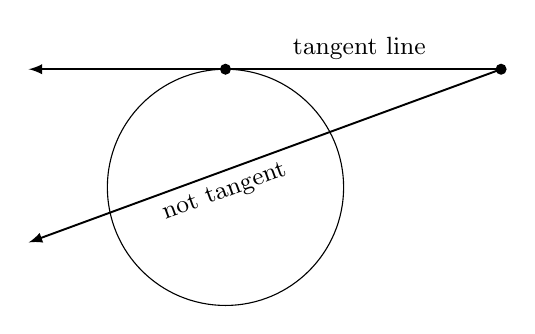
\begin{tikzpicture}
  \draw (0,0) circle (1.5);
  \draw [line width=0.7pt,latex-] (-2.5,1.5) -- (3.5,1.5)
   node [pos=0.7,above] {\small tangent line};
  \fill (0,1.5) circle (2pt);
  \fill (3.5,1.5) circle (2pt);
  \draw [line width=0.7pt,-latex] (3.5,1.5) -- (-2.5,-0.7) node [pos=0.6,below,sloped]
   {\small not tangent};
 \end{tikzpicture}\qquad\qquad
  \begin{tikzpicture}[scale=0.65]
   \coordinate (a) at (2in,0in);
   \node [circle,draw] (c) at (0in,0in) [minimum size=1in] {};
   \filldraw[linecolor,fill=fillcolor,fill opacity=0.4,line width=1.5pt] (a) --
    (tangent cs:node=c,point={(a)},solution=1) node [black,fill opacity=1] {\large $\bullet$}
    node [above,black,fill opacity=1] {\small $A$} -- (c.center) --  (a);
   \draw (1in,0in) circle (1in);
   \fill (0in,0in) circle (3pt);
   \fill (1in,0in) circle (3pt);
   \fill (2in,0in) circle (3pt);
   \node [left] at (0in,0in) {\small $O$};
   \node [right] at (2in,0in) {\small $P$};
   \node [below] at (1in,0in) {\small $C$};
  \end{tikzpicture}\piccaptioninside}
 \par\mbox{}\newline\vspace{1mm}\picskip{0}
  On a sheet of paper draw a circle of radius 1 inch, and call the center of that circle $O$. Pick
  a point $P$ which is $2.5$ inches away from $O$. Draw the circle which has $\overline{OP}$ as a
  diameter, as in the picture on the right in Figure \ref{fig:tanline}. Let $A$ be one of the points
  where this circle intersects the first circle. Draw the line through $P$ and $A$. In general the
  tangent line through a point on a circle is perpendicular to the line joining that point
  to the center of the circle (why?). Use this fact to explain
  why the line you drew is the tangent line through $A$ and to calculate the length
  of $\overline{PA}$. Does it match the physical measurement of $\overline{PA}$?
 \parpic[r]{\begin{tikzpicture}[scale=0.68]
  \filldraw [linecolor,fill=fillcolor,line width=1.5pt] (-2,0) -- (2,0) -- (70:2) -- (-2,0);
  \draw [line width=0.5pt] (0,0) circle (2);
  \node [left] at (-2,0) {\small $A$};
  \node [right] at (2,0) {\small $B$};
  \node [above] at (70:2) {\small $C$};
  \node [below] at (0,0) {\small $O$};
  \draw [dashed] (-2,0) -- (250:2);
  \draw [dashed] (250:2) -- (2,0);
  \fill (-2,0) circle (2.9pt);
  \fill (2,0) circle (2.9pt);
  \fill (70:2) circle (2.9pt);
  \fill (0,0) circle (2.9pt);
 \end{tikzpicture}}
 \item Suppose that $\triangle\,ABC$ is a triangle with side $\overline{AB}$ a diameter of a circle
  with center $O$, as in the picture on the right, and suppose that the vertex $C$ lies on the
  circle. Now imagine that you rotate the circle $180\Degrees$ around its center, so that
  $\triangle\,ABC$ is in a new position, as indicated by the dashed lines in the picture. Explain
  how this picture proves Thales' Theorem.
\end{enumerate}}

\newpage
%Begin Section 1.2
\section{Trigonometric Functions of an Acute Angle}
\parpic[r]{\begin{tikzpicture}[scale=0.5]
   \fill [fill=fillcolor] (0,0) -- (4,0) -- (4,3) -- (0,0);
   \draw [line width=0.5pt] (3.6,0) -- (3.6,0.4) -- (4,0.4);
   \draw [linecolor,line width=1.5pt] (0,0) -- (4,0) -- (4,3) -- cycle;
   \node [below left] at (0,0) {\small $A$};
   \node [below right] at (4,0) {\small $C$};
   \node [above right] at (4,3) {\small $B$};
   \node [below] at (2,0) {\small $b$};
   \node [below] at (2,-0.7) {\small adjacent};
   \node [right] at (4,1.5) {\small $a$};
   \node [rotate=-90,above] at (4.5,1.7) {\small opposite};
   \node [above left] at (2,1.5) {\small $c$};
   \node [rotate=36.87,above] at (1.7,2.1) {\small hypotenuse};
  \end{tikzpicture}}
Consider a right triangle $\triangle\,ABC$, with the right angle at $C$ and with lengths $a$, $b$,
and $c$, as in the figure on the right. For the acute angle $A$, call the leg $\overline{BC}$ its
\textbf{opposite side}, and call the leg $\overline{AC}$ its \textbf{adjacent side}. Recall
that the hypotenuse of the triangle is the side $\overline{AB}$. The ratios of sides of a right
triangle occur often enough in practical applications to warrant their own names, so we define the
six \textbf{trigonometric functions}\index{trigonometric functions} of $A$ as follows:

\begin{table}[h]\centering
\caption{\quad \textbf{The six trigonometric functions of $A$}}\vspace{3mm}
\statecomment{\begin{tabular}{rccrccrcl}\\[0.1pt]
\multicolumn{2}{c}{\textbf{Name of function}\qquad\qquad} & \multicolumn{3}{c}{\textbf{Abbreviation}} & \multicolumn{3}{c}{\textbf{Definition}}\\[7pt]
sine $A$ & {} & {} & $\sin\;A$ & {} & $=$ & $\dfrac{\text{opposite side}}{\text{hypotenuse}}$ & $=$ & $\dfrac{a}{c}$\\[1pt]\\
cosine $A$ & {} & {} & $\cos\;A$ & {} & $=$ & $\dfrac{\text{adjacent side}}{\text{hypotenuse}}$ & $=$ & $\dfrac{b}{c}$\\[1pt]\\
tangent $A$ & {} & {} & $\tan\;A$ & {} & $=$ & $\dfrac{\text{opposite side}}{\text{adjacent side}}$ & $=$ & $\dfrac{a}{b}$\\[1pt]\\
cosecant $A$ & {} & {} & $\csc\;A$ & {} & $=$ & $\dfrac{\text{hypotenuse}}{\text{opposite side}}$ & $=$ & $\dfrac{c}{a}$\\[1pt]\\
secant $A$ & {} & {} & $\sec\;A$ & {} & $=$ & $\dfrac{\text{hypotenuse}}{\text{adjacent side}}$ & $=$ & $\dfrac{c}{b}$\\[1pt]\\
cotangent $A$ & {} & {} & $\cot\;A$ & {} & $=$ & $\dfrac{\text{adjacent side}}{\text{opposite side}}$ & $=$ & $\dfrac{b}{a}$\\[0.1pt]\\
\end{tabular}\label{tbl:funcs}}
\end{table}

We will usually use the abbreviated names of the functions.\index{sine}\index{cosine}\index{tangent}
Notice from Table \ref{tbl:funcs} that the pairs $\sin\;A$ and $\csc\;A$, $\cos\;A$ and $\sec\;A$,
and $\tan\;A$ and $\cot\;A$ are
reciprocals:\index{cosecant}\index{secant}\index{cotangent}\vspace{2mm}

\begin{center}\statecomment{\begin{displaymath}
 \csc\;A ~=~ \dfrac{1}{\sin\;A} \qquad\qquad
 \sec\;A ~=~ \dfrac{1}{\cos\;A} \qquad\qquad
 \cot\;A ~=~ \dfrac{1}{\tan\;A}
\end{displaymath}\vspace{1mm}
\begin{displaymath}
 \sin\;A ~=~ \dfrac{1}{\csc\;A} \qquad\qquad
 \cos\;A ~=~ \dfrac{1}{\sec\;A} \qquad\qquad
 \tan\;A ~=~ \dfrac{1}{\cot\;A}
\end{displaymath}}\end{center}

\begin{exmp}\label{exmp:funcs345}
\parpic[r]{\begin{tikzpicture}[scale=0.4,every node/.style={font=\small}]
   \fill [fill=fillcolor] (0,0) -- (4,0) -- (4,3) -- (0,0);
   \draw [line width=0.5pt] (3.625,0) -- (3.625,0.375) -- (4,0.375);
   \draw [linecolor,line width=1.5pt] (0,0) -- (4,0) -- (4,3) -- cycle;
   \node [below left] at (0,0) {$A$};
   \node [below right] at (4,0) {$C$};
   \node [above right] at (4,3) {$B$};
   \node [below] at (2,0) {$4$};
   \node [right] at (4,1.5) {$3$};
   \node [above left] at (2,1.5) {$5$};
\end{tikzpicture}}
\noindent For the right triangle $\triangle\,ABC$ shown on the right, find the values of all six
 trigonometric functions of the acute angles $A$ and $B$.\vspace{1mm}
 \par\noindent\textbf{Solution:} The hypotenuse of $\triangle\,ABC$ has length $5$. For angle $A$,
 the opposite side $\overline{BC}$ has length $3$ and the adjacent side $\overline{AC}$ has length
 $4$. Thus:
\picskip{2}
 \begin{displaymath}
  \sin\;A ~=~ \dfrac{\text{opposite}}{\text{hypotenuse}} ~=~ \dfrac{3}{5} \qquad\qquad
  \cos\;A ~=~ \dfrac{\text{adjacent}}{\text{hypotenuse}} ~=~ \dfrac{4}{5} \qquad\qquad
  \tan\;A ~=~ \dfrac{\text{opposite}}{\text{adjacent}} ~=~ \dfrac{3}{4}\vspace{2mm}
 \end{displaymath}
 \begin{displaymath}
  \csc\;A ~=~ \dfrac{\text{hypotenuse}}{\text{opposite}} ~=~ \dfrac{5}{3} \qquad\qquad
  \sec\;A ~=~ \dfrac{\text{hypotenuse}}{\text{adjacent}} ~=~ \dfrac{5}{4} \qquad\qquad
  \cot\;A ~=~ \dfrac{\text{adjacent}}{\text{opposite}} ~=~ \dfrac{4}{3}
 \end{displaymath}\vspace{2mm}
 
 \par\noindent For angle $B$, the opposite side $\overline{AC}$ has length $4$ and the adjacent
 side $\overline{BC}$ has length $3$. Thus:
 \begin{displaymath}
  \sin\;B ~=~ \dfrac{\text{opposite}}{\text{hypotenuse}} ~=~ \dfrac{4}{5} \qquad\qquad
  \cos\;B ~=~ \dfrac{\text{adjacent}}{\text{hypotenuse}} ~=~ \dfrac{3}{5} \qquad\qquad
  \tan\;B ~=~ \dfrac{\text{opposite}}{\text{adjacent}} ~=~ \dfrac{4}{3}\vspace{2mm}
 \end{displaymath}
 \begin{displaymath}
  \csc\;B ~=~ \dfrac{\text{hypotenuse}}{\text{opposite}} ~=~ \dfrac{5}{4} \qquad\qquad
  \sec\;B ~=~ \dfrac{\text{hypotenuse}}{\text{adjacent}} ~=~ \dfrac{5}{3} \qquad\qquad
  \cot\;B ~=~ \dfrac{\text{adjacent}}{\text{opposite}} ~=~ \dfrac{3}{4}
 \end{displaymath}
\end{exmp}
\divider
\vspace{3mm}

Notice in Example \ref{exmp:funcs345} that we did not specify the units for the lengths. This
raises the possibility that our answers depended on a triangle of a specific physical size.

For example, suppose that two different
students are reading this textbook: one in the United States and one in Germany. The American
student thinks that the lengths $3$, $4$, and $5$ in Example \ref{exmp:funcs345}
are measured in inches, while the German student thinks that they are measured in centimeters.
Since $1$ in $\approx$ $2.54$ cm, the students are using triangles of different physical sizes (see
Figure \ref{fig:similar} below, not drawn to scale).

\begin{figure}[h]
 \centering
 \subfloat[][ Inches]{
  \begin{tikzpicture}[scale=0.9,every node/.style={font=\small}]
   \fill [fill=fillcolor] (0,0) -- (4,0) -- (4,3) -- cycle;
   \draw [line width=0.5pt] (3.7,0) -- (3.7,0.3) -- (4,0.3);
   \draw [linecolor,line width=1.5pt] (0,0) -- (4,0) -- (4,3) -- cycle;
   \node [below left] at (0,0) {$A$};
   \node [above right] at (4,3) {$B$};
   \node [below right] at (4,0) {$C$};
   \node [right] at (4,1.5) {$3$};
   \node [below] at (2,0) {$4$};
   \node [above left] at (2,1.5) {$5$};
  \end{tikzpicture}}
 \qquad
 \subfloat[][ Centimeters]{
  \begin{tikzpicture}[scale=0.9,every node/.style={font=\small}]
   \fill [fill=fillcolor] (0,0) -- (1.6,0) -- (1.6,1.2) -- cycle;
   \draw [line width=0.5pt] (1.4,0) -- (1.4,0.2) -- (1.6,0.2);
   \draw [linecolor,line width=1.5pt] (0,0) -- (1.6,0) -- (1.6,1.2) -- cycle;
   \node [below left] at (0,0) {$A'$};
   \node [above right] at (1.6,1.2) {$B'$};
   \node [below right] at (1.6,0) {$C'$};
   \node [right] at (1.6,0.6) {$3$};
   \node [below] at (0.8,0) {$4$};
   \node [above left] at (0.8,0.6) {$5$};
  \end{tikzpicture}}
 \qquad
 \subfloat[][ Similar triangles]{
  \begin{tikzpicture}[scale=0.9,every node/.style={font=\small}]
   \fill [fill=fillcolor] (0,0) -- (4,0) -- (4,3) -- cycle;
   \draw [line width=0.5pt] (3.7,0) -- (3.7,0.3) -- (4,0.3);
   \draw [line width=0.5pt] (1.4,0) -- (1.4,0.2) -- (1.6,0.2);
   \draw [linecolor,line width=1.5pt] (1.6,0) -- (1.6,1.2);
   \draw [linecolor,line width=1.5pt] (0,0) -- (4,0) -- (4,3) -- cycle;
   \node [above left] at (0,0) {$A$};
   \node [below left] at (0,0) {$A'$};
   \node [above right] at (4,3) {$B$};
   \node [above] at (1.6,1.2) {$B'$};
   \node [below right] at (4,0) {$C$};
   \node [below] at (1.6,0) {$C'$};
  \end{tikzpicture}}
 \caption[]{\quad $\triangle\,ABC ~\sim~ \triangle\,A'B'C'$}
 \label{fig:similar}
\end{figure}

If the American triangle is $\triangle\,ABC$ and the German triangle is $\triangle\,A'B'C'$, then
we see from Figure \ref{fig:similar} that $\triangle\,ABC$ is similar to $\triangle\,A'B'C'$, and
hence the corresponding angles are equal and the ratios of the corresponding sides are equal. In
fact, we know that common ratio: the sides of $\triangle\,ABC$ are approximately $2.54$ times longer
than the corresponding sides of $\triangle\,A'B'C'$. So when the American student calculates
$\sin\;A$ and the German student calculates $\sin\;A'$, they get the same answer:\footnote{We will
use the notation $AB$ to denote the length of a line segment $\overline{AB}$.}\index{length of a
line segment}
\begin{displaymath}
 \triangle\,ABC ~\sim~ \triangle\,A'B'C' \quad\Rightarrow\quad
 \dfrac{BC}{B'C'} ~=~ \dfrac{AB}{A'B'} \quad\Rightarrow\quad
 \dfrac{BC}{AB} ~=~ \dfrac{B'C'}{A'B'} \quad\Rightarrow\quad \sin\;A ~=~ \sin\;A'
\end{displaymath}
Likewise, the other values of the trigonometric functions of $A$ and $A'$
are the same. In fact, our argument was general enough to work with any similar
right triangles. This leads us to the following conclusion:\vspace{1mm}

\begin{center}\statecomment[0.85\textwidth]{
When calculating the trigonometric functions of an acute angle $A$, you may use \emph{any} right
triangle which has $A$ as one of the angles.}\end{center}

Since we defined the trigonometric functions in terms of ratios of sides, you can think of the
units of measurement for those sides as canceling out in those ratios. This means that \emph{the
values of the trigonometric functions are unitless numbers}. So when the American student
calculated $3/5$ as the value of $\sin\;A$ in Example \ref{exmp:funcs345}, that is the same as
the $3/5$ that the German student calculated, despite the different units for the
lengths of the sides.

\begin{exmp}\label{exmp:funcs45}
\parpic[r]{\begin{tikzpicture}
 \fill [fill=fillcolor] (0,0) -- (2,0) -- (2,2) -- cycle;
 \draw [line width=0.5pt] (1.8,0) -- (1.8,0.2) -- (2,0.2);
 \draw [linecolor,line width=1.5pt] (0,0) -- (2,0) -- (2,2) -- (0,2) -- cycle;
 \draw [linecolor,line width=1.5pt] (0,0) -- (2,2);
 \node [below left] at (0,0) {\small $A$};
 \node [above right] at (2,2) {\small $B$};
 \node [below right] at (2,0) {\small $C$};
 \node [right] at (2,1) {\small $1$};
 \node [below] at (1,0) {\small $1$};
 \node [left] at (0,1) {\small $1$};
 \node [above] at (1,2) {\small $1$};
 \node [above left] at (1.1,1) {\small $\sqrt{2}$};
 \node at (0.6,0.2) {\small $45\Degrees$};
\end{tikzpicture}}
\noindent Find the values of all six trigonometric functions of $45\Degrees$.\vspace{1mm}
 \par\noindent\textbf{Solution:} Since we may use any right triangle which has $45\Degrees$ as one of
 the angles, use the simplest one: take a square whose sides are all $1$ unit long and divide it
 in half diagonally, as in the figure on the right. Since the two legs of the triangle
 $\triangle\,ABC$ have the same length, $\triangle\,ABC$ is an isosceles triangle, which means
 that the angles $A$ and $B$ are equal. So since $A + B = 90\Degrees$, this means that we must have
 $A = B = 45\Degrees$. By the Pythagorean Theorem, the length $c$ of the hypotenuse is given by
 \begin{displaymath}
  c^2 ~=~ 1^2 ~+~ 1^2 ~=~ 2 \quad\Rightarrow\quad c ~=~ \sqrt{2} ~.
 \end{displaymath}
 Thus, using the angle $A$ we get:
 \begin{displaymath}
  \sin\;45\Degrees ~=~ \dfrac{\text{opposite}}{\text{hypotenuse}} ~=~ \dfrac{1}{\sqrt{2}} \quad\quad
  \cos\;45\Degrees ~=~ \dfrac{\text{adjacent}}{\text{hypotenuse}} ~=~ \dfrac{1}{\sqrt{2}} \quad\quad
  \tan\;45\Degrees ~=~ \dfrac{\text{opposite}}{\text{adjacent}} ~=~ \dfrac{1}{1} ~=~ 1\vspace{2mm}
 \end{displaymath}
 \begin{displaymath}
  \csc\;45\Degrees ~=~ \dfrac{\text{hypotenuse}}{\text{opposite}} ~=~ \sqrt{2} \quad\quad
  \sec\;45\Degrees ~=~ \dfrac{\text{hypotenuse}}{\text{adjacent}} ~=~ \sqrt{2} \quad\quad
  \cot\;45\Degrees ~=~ \dfrac{\text{adjacent}}{\text{opposite}} ~=~ \dfrac{1}{1} ~=~ 1\vspace{2mm}
 \end{displaymath}
 Note that we would have obtained the same answers if we had used any right triangle similar to
 $\triangle\,ABC$. For example, if we multiply each side of $\triangle\,ABC$ by $\sqrt{2}$, then
 we would have a similar triangle with legs of length $\sqrt{2}$ and hypotenuse of length $2$. This
 would give us $\sin\;45\Degrees = \frac{\sqrt{2}}{2}$, which equals
 $\frac{\sqrt{2}}{\sqrt{2} \cdot \sqrt{2}} = \frac{1}{\sqrt{2}}$ as before. The same goes for
 the other functions.
\end{exmp}\vspace{-2mm}
\divider
\newpage
\begin{exmp}\label{exmp:funcs60}
\parpic[r]{\begin{tikzpicture}
 \fill [fill=fillcolor] (0,0) -- (1.5,0) -- (1.5,2.598) -- cycle;
 \draw [line width=0.5pt] (1.2,0) -- (1.2,0.3) -- (1.5,0.3);
 \draw [linecolor,line width=1.5pt] (0,0) -- (3,0) -- (1.5,2.598) -- cycle;
 \draw [linecolor,line width=1.5pt] (1.5,0) -- (1.5,2.598);
 \node [below left] at (0,0) {\small $A$};
 \node [above] at (1.5,2.598) {\small $B$};
 \node [below] at (1.5,0) {\small $C$};
 \node [below] at (0.75,0) {\small $1$};
 \node [below] at (2.25,0) {\small $1$};
 \node [above left] at (0.75,1.2) {\small $2$};
 \node [above right] at (2.25,1.2) {\small $2$};
 \node [right] at (1.5,0.866) {\small $\sqrt{3}$};
 \node at (0.45,0.2) {\small $60\Degrees$};
 \node at (2.45,0.2) {\small $60\Degrees$};
 \node at (1.2,1.5) {\small $30\Degrees$};
 \draw [decorate,decoration={brace,raise=10pt,mirror},segment amplitude=3mm] (0,0) -- (3,0);
 \node [below] at (1.5,-0.75) {\small $2$}; 
\end{tikzpicture}}
%\picskip{9}
\noindent Find the values of all six trigonometric functions of $60\Degrees$.\vspace{1mm}
 \par\noindent\textbf{Solution:} Since we may use any right triangle which has $60\Degrees$ as one of
 the angles, we will use a simple one: take a triangle whose sides are all $2$ units long and divide
 it in half by drawing the bisector from one vertex to the opposite side, as in the figure on the
 right. Since the original triangle was an
 \emph{equilateral triangle}\index{equilateral triangle}\index{triangle!equilateral} (i.e.
 all three sides had the same length), its three angles were all the same, namely $60\Degrees$.
 Recall from elementary geometry that the bisector from the vertex angle of an equilateral triangle
 to its opposite side bisects both the vertex angle and the opposite side. So as in the figure on
 the right, the triangle $\triangle\,ABC$ has angle $A = 60\Degrees$ and angle $B = 30\Degrees$,
 which forces the angle $C$ to be $90\Degrees$. Thus, $\triangle\,ABC$ is a right triangle. We see
 that the hypotenuse has length $c = AB = 2$ and the leg $\overline{AC}$ has length $b = AC = 1$.
 By the Pythagorean Theorem, the length $a$ of the leg $\overline{BC}$ is given by
 \begin{displaymath}
  a^2 ~+~ b^2 ~=~ c^2 \quad\Rightarrow\quad a^2 ~=~ 2^2 ~-~ 1^2 ~=~ 3
   \quad\Rightarrow\quad a ~=~ \sqrt{3} ~.
 \end{displaymath}
 Thus, using the angle $A$ we get:
 \begin{displaymath}
  \sin\;60\Degrees \;=\; \dfrac{\text{opposite}}{\text{hypotenuse}} \;=\; \dfrac{\sqrt{3}}{2} \qquad
  \cos\;60\Degrees \;=\; \dfrac{\text{adjacent}}{\text{hypotenuse}} \;=\; \dfrac{1}{2} \qquad
  \tan\;60\Degrees \;=\; \dfrac{\text{opposite}}{\text{adjacent}} \;=\; \dfrac{\sqrt{3}}{1} \,=\,
   \sqrt{3}\vspace{2mm}
 \end{displaymath}
 \begin{displaymath}
  \csc\;60\Degrees \;=\; \dfrac{\text{hypotenuse}}{\text{opposite}} \;=\; \dfrac{2}{\sqrt{3}} \qquad
  \sec\;60\Degrees \;=\; \dfrac{\text{hypotenuse}}{\text{adjacent}} \;=\; 2 \qquad
  \cot\;60\Degrees \;=\; \dfrac{\text{adjacent}}{\text{opposite}} \;=\;
   \dfrac{1}{\sqrt{3}}~\quad\quad\vspace{2mm}
 \end{displaymath}
 Notice that, as a bonus, we get the values of all six trigonometric functions of $30\Degrees$, by
 using angle $B = 30\Degrees$ in the same triangle $\triangle\,ABC$ above:
 \begin{displaymath}
  \sin\;30\Degrees \;=\; \dfrac{\text{opposite}}{\text{hypotenuse}} \;=\; \dfrac{1}{2} \qquad
  \cos\;30\Degrees \;=\; \dfrac{\text{adjacent}}{\text{hypotenuse}} \;=\; \dfrac{\sqrt{3}}{2} \qquad
  \tan\;30\Degrees \;=\; \dfrac{\text{opposite}}{\text{adjacent}} \;=\;
   \dfrac{1}{\sqrt{3}}\quad\quad\vspace{2mm}
 \end{displaymath}
 \begin{displaymath}
  \csc\;30\Degrees \;=\; \dfrac{\text{hypotenuse}}{\text{opposite}} \;=\; 2 \qquad
  \sec\;30\Degrees \;=\; \dfrac{\text{hypotenuse}}{\text{adjacent}} \;=\; \dfrac{2}{\sqrt{3}} \qquad
  \cot\;30\Degrees \;=\; \dfrac{\text{adjacent}}{\text{opposite}} \;=\;
   \dfrac{\sqrt{3}}{1} \;=\; \sqrt{3}\vspace{2mm}
 \end{displaymath}
\end{exmp}\vspace{-7mm}
\begin{exmp}\label{exmp:ex1.8}
\parpic[r]{\begin{tikzpicture}
 \fill [fill=fillcolor] (0,0) -- (1.6,0) -- (1.6,1.2) -- cycle;
 \draw [line width=0.5pt] (1.4,0) -- (1.4,0.2) -- (1.6,0.2);
 \draw [linecolor,line width=1.5pt] (0,0) -- (1.6,0) -- (1.6,1.2) -- cycle;
 \node [below left] at (0,0) {\small $A$};
 \node [above right] at (1.6,1.2) {\small $B$};
 \node [below right] at (1.6,0) {\small $C$};
 \node [right] at (1.6,0.6) {\small $2$};
 \node [below] at (0.8,0) {\small $b$};
 \node [above left] at (0.8,0.6) {\small $3$};
 \end{tikzpicture}}
%\picskip{3}
\noindent $A$ is an acute angle such that $\sin\;A = \frac{2}{3}$. Find the values of the other trigonometric
 functions of $A$.\vspace{1mm}
 \par\noindent\textbf{Solution:} In general it helps to draw a right triangle to solve problems of
 this type. The reason is that the trigonometric functions were defined in terms of ratios of
 sides of a right triangle, and you are given one such function (the sine, in this case)
 already in terms of a ratio: $\sin\;A = \frac{2}{3}$. Since $\sin\;A$ is defined as
 $\frac{\text{opposite}}{\text{hypotenuse}}$, use $2$ as the length of the side opposite $A$ and use
 $3$ as the length of the hypotenuse in a right triangle $\triangle\,ABC$ (see the figure above), so
 that $\sin\;A = \frac{2}{3}$.
 The adjacent side to $A$ has unknown length $b$, but we can use the Pythagorean Theorem to find it:
 \begin{displaymath}
  2^2 ~+~ b^2 ~=~ 3^2 \quad\Rightarrow\quad b^2 ~=~ 9 ~-~ 4 ~=~ 5 \quad\Rightarrow\quad
   b ~=~ \sqrt{5}
 \end{displaymath}
 We now know the lengths of all sides of the triangle $\triangle\,ABC$, so we have:
 \begin{displaymath}
  \cos\;A \;=\; \dfrac{\text{adjacent}}{\text{hypotenuse}} \;=\; \dfrac{\sqrt{5}}{3} \qquad
  \tan\;A \;=\; \dfrac{\text{opposite}}{\text{adjacent}} \;=\;
   \dfrac{2}{\sqrt{5}}\quad\quad\vspace{2mm}
 \end{displaymath}
 \begin{displaymath}
  \csc\;A \;=\; \dfrac{\text{hypotenuse}}{\text{opposite}} \;=\; \dfrac{3}{2} \qquad
  \sec\;A \;=\; \dfrac{\text{hypotenuse}}{\text{adjacent}} \;=\; \dfrac{3}{\sqrt{5}} \qquad
  \cot\;A \;=\; \dfrac{\text{adjacent}}{\text{opposite}} \;=\; \dfrac{\sqrt{5}}{2}\vspace{2mm}
 \end{displaymath}
\end{exmp}\vspace{-2mm}
\divider
\vspace{2mm}

You may have noticed the connections between the sine and cosine, secant and cosecant, and tangent
and cotangent of the complementary angles in Examples \ref{exmp:funcs345} and \ref{exmp:funcs60}.
Generalizing those examples gives us the following theorem:\index{Cofunction theorem}

\statethm{thm:cofunction}{
\textbf{Cofunction Theorem:} If $A$ and $B$ are the complementary acute angles in a right triangle
$\triangle\,ABC$, then the following relations hold:
\begin{displaymath}
\sin\;A ~=~ \cos\;B \qquad\qquad \sec\;A ~=~ \csc\;B \qquad\qquad \tan\;A ~=~ \cot\;B
\end{displaymath}
\begin{displaymath}
\sin\;B ~=~ \cos\;A \qquad\qquad \sec\;B ~=~ \csc\;A \qquad\qquad \tan\;B ~=~ \cot\;A
\end{displaymath}
We say that the pairs of functions $\lbrace\;\sin, \cos\;\rbrace$, $\lbrace\;\sec, \csc\;\rbrace$,
and $\lbrace\;\tan, \cot\;\rbrace$ are \textbf{cofunctions}.\index{cofunctions}}

So sine and cosine are cofunctions, secant and cosecant are cofunctions, and tangent and cotangent
are cofunctions. That is how the functions cosine, cosecant, and cotangent got the ``co'' in their
names. The Cofunction Theorem says that any trigonometric function of an acute angle is equal to
its cofunction of the complementary angle.\vspace{1mm}

\begin{exmp}
 Write each of the following numbers as trigonometric functions of an angle less than $45\Degrees$:
\textbf{(a)} $\sin\;65\Degrees$; \textbf{(b)} $\cos\;78\Degrees$; \textbf{(c)}
 $\tan\;59\Degrees$.\vspace{1mm}
\par\noindent\textbf{Solution:} \textbf{(a)} The complement of $65\Degrees$ is $90\Degrees -
 65\Degrees = 25\Degrees$ and the cofunction of $\sin$ is $\cos$, so by the Cofunction Theorem we
 know that $\sin\;65\Degrees = \cos\;25\Degrees$.

\par\noindent \textbf{(b)} The complement of $78\Degrees$ is $90\Degrees - 78\Degrees =
12\Degrees$ and the cofunction of $\cos$ is $\sin$, so $\cos\;78\Degrees = \sin\;12\Degrees$.

\par\noindent \textbf{(c)} The complement of $59\Degrees$ is $90\Degrees - 59\Degrees =
31\Degrees$ and the cofunction of $\tan$ is $\cot$, so $\tan\;59\Degrees = \cot\;31\Degrees$.
\end{exmp}\vspace{-2mm}
\divider

\begin{figure}[h]
 \centering
 \subfloat[][ $45-45-90$]{
 \begin{tikzpicture}[every node/.style={font=\small}]
  \draw [line width=0.5pt] (1.1,0) -- (1.1,0.2) -- (1.3,0.2);
  \draw [linecolor,line width=1.5pt] (0,0) -- (1.3,0) -- (1.3,1.3) -- cycle;
  \node [below] at (0.65,0) {$a$};
  \node [right] at (1.3,0.65) {$a$};
  \node [above left] at (0.65,0.65) {$a\sqrt{2}$};
  \node at (0.5,0.2) {$45\Degrees$};
  \node at (1.05,0.75) {$45\Degrees$};
 \end{tikzpicture}}
 \qquad\qquad
 \subfloat[][ $30-60-90$]{
 \begin{tikzpicture}[every node/.style={font=\small}]
  \draw [line width=0.5pt] (2.05,0) -- (2.05,0.2) -- (2.25,0.2);
  \draw [linecolor,line width=1.5pt] (0,0) -- (2.25,0) -- (2.25,1.3) -- cycle;
  \node [below] at (1.125,0) {$a\sqrt{3}$};
  \node [right] at (2.25,0.65) {$a$};
  \node [above left] at (1.125,0.65) {$2a$};
  \node at (0.8,0.2) {$30\Degrees$};
  \node at (1.95,0.85) {$60\Degrees$};
 \end{tikzpicture}}
 \caption[]{\quad Two general right triangles (any $a>0$)}
 \label{fig:gen45}
\end{figure}

The angles $30\Degrees$, $45\Degrees$, and $60\Degrees$ arise often in applications. We can use the
Pythagorean Theorem to generalize the right triangles in
Examples \ref{exmp:funcs45} and \ref{exmp:funcs60} and see what \emph{any}
$45-45-90$ and $30-60-90$ right triangles look like, as in Figure \ref{fig:gen45} above.
\newpage
\begin{exmp}\label{exmp:funcs75}
\parpic[r]{\begin{tikzpicture}[scale=0.65,every node/.style={font=\small}]
  \draw [dashed] (2.536,0) -- (2.536,9.464);
  \draw [dashed] (2.536,6) -- (6,6);
  \draw [linecolor] (5.6,0) -- (5.6,0.4) -- (6,0.4);
  \draw [linecolor,rotate around={45:(6,6)}] (5.6,6) -- (5.6,6.4) -- (6,6.4);
  \draw (2.136,0) -- (2.136,0.4) -- (2.536,0.4);
  \draw (2.936,6) -- (2.936,6.4) -- (2.536,6.4);
  \draw [linecolor,line width=1.5pt] (0,0) -- (6,0) -- (6,6) -- (2.536,9.464) -- cycle;
  \draw [linecolor,line width=1.5pt] (0,0) -- (6,6) node [black,sloped,above,pos=0.6] {$\sqrt{3}$}
   node [black,sloped,above,pos=0.17] {$30\Degrees$};
  \node [left] at (0,0) {$A$};
  \node [right] at (6,6) {$B$};
  \node [right] at (6,0) {$C$};
  \node [above] at (2.536,9.464) {$D$};
  \node [above right] at (2.536,0) {$E$};
  \node [below left] at (2.536,6) {$F$};
  \node [below] at (3,0) {$\sqrt{\frac{3}{2}}$};
  \node [right] at (6,3) {$\sqrt{\frac{3}{2}}$};
  \node [left] at (1.2,4.7) {$2$};
  \node [right] at (4.5,7.732) {$1$};
  \node at (0.8,0.3) {$45\Degrees$};
 \end{tikzpicture}}
%\picskip{18}
\noindent Find the sine, cosine, and tangent of $75\Degrees$.\vspace{1mm}
\par\noindent\textbf{Solution:} Since
$75\Degrees = 45\Degrees + 30\Degrees$, place a $30-60-90$ right triangle $\triangle\,ADB$ with
legs of length $\sqrt{3}$ and $1$ on top of the hypotenuse of a $45-45-90$ right triangle
$\triangle\,ABC$ whose hypotenuse has length $\sqrt{3}$, as in the figure on the right.
From Figure \ref{fig:gen45}(a) we know that the length of each leg of $\triangle\,ABC$
is the length of the hypotenuse divided by $\sqrt{2}$. So $AC = BC = \frac{\sqrt{3}}{\sqrt{2}} =
\sqrt{\frac{3}{2}}$. Draw $\overline{DE}$ perpendicular to $\overline{AC}$, so that $\triangle\,ADE$
is a right triangle. Since $\angle\,BAC = 45\Degrees$ and $\angle\,DAB = 30\Degrees$, we see that
$\angle\,DAE = 75\Degrees$ since it is the sum of those two angles. Thus, we need to find the sine,
cosine, and tangent of $\angle\,DAE$.
\picskip{6}
Notice that $\angle\,ADE = 15\Degrees$, since it is the complement of $\angle\,DAE$. And
$\angle\,ADB = 60\Degrees$, since it is the complement of $\angle\,DAB$. Draw
$\overline{BF}$ perpendicular to $\overline{DE}$, so that $\triangle\,DFB$ is a right triangle. Then
$\angle\,BDF = 45\Degrees$, since it is the difference of $\angle\,ADB = 60\Degrees$ and
$\angle\,ADE = 15\Degrees$. Also, $\angle\,DBF = 45\Degrees$ since it is the complement of
$\angle\,BDF$. The hypotenuse $\overline{BD}$ of $\triangle\,DFB$ has length $1$ and
$\triangle\,DFB$ is a $45-45-90$ right triangle, so we know that $DF = FB = \frac{1}{\sqrt{2}}$.

Now, we know that $\overline{DE} \perp \overline{AC}$ and $\overline{BC} \perp \overline{AC}$, so
$\overline{FE}$ and $\overline{BC}$ are parallel. Likewise, $\overline{FB}$ and $\overline{EC}$ are
both perpendicular to $\overline{DE}$ and hence $\overline{FB}$ is parallel to $\overline{EC}$.
Thus, $FBCE$ is a rectangle, since $\angle\,BCE$ is a right angle. So $EC = FB = \frac{1}{\sqrt{2}}$
and $FE = BC = \sqrt{\frac{3}{2}}$. Hence,
\begin{displaymath}
 DE ~=~ DF ~+~ FE ~=~ \tfrac{1}{\sqrt{2}} ~+~ \sqrt{\tfrac{3}{2}} ~=~ \tfrac{\sqrt{3} ~+~ 1}{\sqrt{2}}
 \quad\text{and}\quad
 AE ~=~ AC ~-~ EC ~=~ \sqrt{\tfrac{3}{2}} ~-~ \tfrac{1}{\sqrt{2}} ~=~ \tfrac{\sqrt{3} ~-~ 1}{\sqrt{2}}
 ~. ~\text{ Thus,}
\end{displaymath}
\begin{displaymath}
 \sin\;75\Degrees = \tfrac{DE}{AD} = \tfrac{\frac{\sqrt{3} + 1}{\sqrt{2}}}{2} =
 \tfrac{\sqrt{6} + \sqrt{2}}{4} ~,~ \cos\;75\Degrees = \tfrac{AE}{AD} =
 \tfrac{\frac{\sqrt{3} - 1}{\sqrt{2}}}{2} = \tfrac{\sqrt{6} - \sqrt{2}}{4}
 ~,~\text{and} ~ \tan\;75\Degrees =
 \tfrac{DE}{AE} = \tfrac{\frac{\sqrt{3} + 1}{\sqrt{2}}}{\frac{\sqrt{3} - 1}{\sqrt{2}}} =
 \tfrac{\sqrt{6} + \sqrt{2}}{\sqrt{6} - \sqrt{2}} ~.
\end{displaymath}
Note: Taking reciprocals, we get $\csc\;75\Degrees = \frac{4}{\sqrt{6} + \sqrt{2}}$,
$\sec\;75\Degrees = \frac{4}{\sqrt{6} - \sqrt{2}}$, and 
$\cot\;75\Degrees = \frac{\sqrt{6} - \sqrt{2}}{\sqrt{6} + \sqrt{2}}$.
\end{exmp}\vspace{-2mm}
\divider
\vspace{3mm}

\startexercises\label{sec1dot2}
\vspace{3mm}
{\small
\piccaption[]{\label{fig:exer1.2.1}}\parpic[r]{\begin{tikzpicture}[scale=0.90,every node/.style={font=\small}]
 \fill [fill=fillcolor] (0,0) -- (1.6,0) -- (1.6,1.2) -- cycle;
 \draw [line width=0.5pt] (1.4,0) -- (1.4,0.2) -- (1.6,0.2);
 \draw [linecolor,line width=1.5pt] (0,0) -- (1.6,0) -- (1.6,1.2) -- cycle;
 \node [below left] at (0,0) {$A$};
 \node [above right] at (1.6,1.2) {$B$};
 \node [below right] at (1.6,0) {$C$};
 \node [right] at (1.6,0.6) {$a$};
 \node [below] at (0.8,0) {$b$};
 \node [above left] at (0.8,0.6) {$c$};
 \end{tikzpicture}}
\picskip{1}
\par\noindent For Exercises 1-10, find the values of all six trigonometric functions of\\angles $A$
and $B$ in the right triangle $\triangle\,ABC$ in Figure \ref{fig:exer1.2.1}.
\begin{enumerate}[\bfseries 1.]
 \begin{multicols}{2}
  \item $a = 5$, $b = 12$, $c = 13$
  \item $a = 8$, $b = 15$, $c = 17$
 \end{multicols}
 \begin{multicols}{2}
  \item $a = 7$, $b = 24$, $c = 25$
  \item $a = 20$, $b = 21$, $c = 29$
 \end{multicols}
 \begin{multicols}{3}
  \item $a = 9$, $b = 40$, $c = 41$
  \item $a = 1$, $b = 2$, $c = \sqrt{5}$
  \item $a = 1$, $b = 3$
 \end{multicols}
 \begin{multicols}{3}
  \item $a = 2$, $b = 5$
  \item $a = 5$, $c = 6$
  \item $b = 7$, $c = 8$
 \end{multicols}
\suspend{enumerate}
\par\noindent For Exercises 11-18, find the values of the other five trigonometric functions of the
acute angle $A$ given the indicated value of one of the functions.
\resume{enumerate}[{[\bfseries 1.]}]
 \begin{multicols}{4}
  \item $\sin\;A = \frac{3}{4}$
  \item $\cos\;A = \frac{2}{3}$
  \item $\cos\;A = \frac{2}{\sqrt{10}}$
  \item $\sin\;A = \frac{2}{4}$
 \end{multicols}
 \begin{multicols}{4}
  \item $\tan\;A = \frac{5}{9}$
  \item $\tan\;A = 3$
  \item $\sec\;A = \frac{7}{3}$
  \item $\csc\;A = 3$
 \end{multicols}
\suspend{enumerate}
\par\noindent For Exercises 19-23, write the given number as a trigonometric function of an acute
angle less than $45\Degrees$.
\resume{enumerate}[{[\bfseries 1.]}]
 \begin{multicols}{5}
  \item $\sin\;87\Degrees$
  \item $\sin\;53\Degrees$
  \item $\cos\;46\Degrees$
  \item $\tan\;66\Degrees$
  \item $\sec\;77\Degrees$
 \end{multicols}
\suspend{enumerate}
\par\noindent For Exercises 24-28, write the given number as a trigonometric function of an acute
angle greater than $45\Degrees$.
\resume{enumerate}[{[\bfseries 1.]}]
 \begin{multicols}{5}
  \item $\sin\;1\Degrees$
  \item $\cos\;13\Degrees$
  \item $\tan\;26\Degrees$
  \item $\cot\;10\Degrees$
  \item $\csc\;43\Degrees$
 \end{multicols}
 \item In Example \ref{exmp:funcs60} we found the values of all six trigonometric functions of
  $60\Degrees$ and $30\Degrees$.
  \begin{enumerate}[\bfseries (a)]
   \begin{multicols}{2}
    \item Does $\;\sin\;30\Degrees ~+~ \sin\;30\Degrees ~=~ \sin\;60\Degrees$?
    \item Does $\;\cos\;30\Degrees ~+~ \cos\;30\Degrees ~=~ \cos\;60\Degrees$?
   \end{multicols}
   \begin{multicols}{2}
    \item Does $\;\tan\;30\Degrees ~+~ \tan\;30\Degrees ~=~ \tan\;60\Degrees$?
    \item Does $\;2\,\sin\;30\Degrees\,\cos\;30\Degrees ~=~ \sin\;60\Degrees$?
   \end{multicols}
  \end{enumerate}
 \item For an acute angle $A$, can $\sin\;A$ be larger than $1$? Explain your answer.
 \item For an acute angle $A$, can $\cos\;A$ be larger than $1$? Explain your answer.
 \item For an acute angle $A$, can $\sin\;A$ be larger than $\tan\;A$? Explain your answer.
 \item If $A$ and $B$ are acute angles and $A < B$, explain why $\sin\;A < \sin\;B$.
 \item If $A$ and $B$ are acute angles and $A < B$, explain why $\cos\;A > \cos\;B$.
 \item Prove the Cofunction Theorem (Theorem \ref{thm:cofunction}). (\emph{Hint: Draw a right
  triangle and label the angles and sides.})
 \item Use Example \ref{exmp:funcs75} to find all six trigonometric functions of $15\Degrees$.
 \piccaption[]{\label{fig:exer1.2.35}}\parpic[r]{\begin{tikzpicture}
  \draw [name path=circle] (0,0) circle (2cm);
  \draw [linecolor,line width=1.5pt,name path=AB] (-2cm,1.92154cm) -- (2cm,0cm) -- (-2cm,0cm) --
   cycle;
  \draw [linecolor,line width=1.5pt,name intersections={of=circle and AB}]
   (intersection-3) -- (intersection-2) node[black,pos=0.65,below] {\small $\enskip\sqrt{3}$};
  \fill [black,name intersections={of=circle and AB}] (intersection-1) circle (2.5pt)
   node[right] {\small $B$} (intersection-2) circle (2.5pt) node[above] {\small $D$};
  \fill (0cm,0cm) circle (2.5pt);
  \fill (-2cm,0cm) circle (2.5pt);
  \fill (-2cm,1.92154cm) circle (2.5pt);
  \node [above left] at (-2cm,1.92154cm) {\small $A$};
  \node [left] at (-2cm,0cm) {\small $C$};
  \node [below] at (0,0) {\small $O$};
  \node [below] at (1cm,0cm) {\small $2$};
 \end{tikzpicture}}
 \item\label{exer:circle1237} In Figure \ref{fig:exer1.2.35}, $\overline{CB}$ is a diameter of a
  circle with a radius of
  $2$ cm and center $O$, $\triangle\,ABC$ is a right triangle, and $\overline{CD}$\\has length
  $\sqrt{3}$ cm.
  \begin{enumerate}[\bfseries (a)]
   \item Find $\;\sin\;A$. (\emph{Hint: Use Thales' Theorem.})
   \item Find the length of $\;\overline{AC}$.
   \item Find the length of $\;\overline{AD}$.
   \item Figure \ref{fig:exer1.2.35} is drawn to scale. Use a protractor to\\ measure
   the angle $A$, then use your calculator to find\\the sine of that angle. Is the
   calculator result close to\\your answer from part(a)?\\Note: Make sure that your
   calculator is in degree mode.
  \end{enumerate}
\suspend{enumerate}
\resume{enumerate}[{[\bfseries 1.]}]
 \item In Exercise \ref{exer:circle1237}, verify that the area of $\triangle\,ABC$ equals
  $\frac{1}{2} AB \cdot CD$. Why does this make sense?\index{area}
 \item In Exercise \ref{exer:circle1237}, verify that the area of $\triangle\,ABC$ equals
  $\frac{1}{2} AB \cdot AC \; \sin\;A$.
 \item In Exercise \ref{exer:circle1237}, verify that the area of $\triangle\,ABC$ equals
  $\frac{1}{2} (BC)^2 \;\cot\;A$.
\end{enumerate}}

\picskip{1}

\newpage
%Begin Section 1.3
\section{Applications and Solving Right Triangles}
Throughout its early development, trigonometry was often used as a means of indirect
measurement, e.g. determining large distances or lengths by using
measurements of angles and small, known distances. Today, trigonometry is widely used in physics,
astronomy, engineering, navigation, surveying, and various
fields of mathematics and other disciplines. In this section we will see some of the ways in which
trigonometry can be applied. Your calculator should be in degree mode for these examples.

\vspace{2mm}
\begin{exmp}
 A person stands $150$ ft away from a flagpole and measures an \emph{angle of
 elevation}\index{angle of elevation} of $32\Degrees$ from his horizontal line of sight to the top
 of the flagpole. Assume that the person's eyes are a vertical distance of 6 ft from the ground.
 What is the height of the flagpole?
\parpic[r]{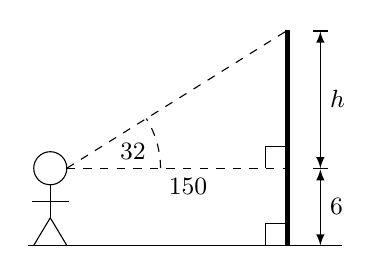
\begin{tikzpicture}[scale=1.4,every node/.style={font=\small}]
 \draw [left] (-0.15,0) circle (0.15);
 \draw (-0.15,-0.15) -- (-0.15,-0.45);
 \draw (-0.15,-0.45) -- (-0.3,-0.7);
 \draw (-0.15,-0.45) -- (0,-0.7);
 \draw (-0.32,-0.3) -- (0.02,-0.3);
 \draw [dashed] (0,0) -- (2,0);
 \node [below] at (1.1,0) {$150$};
 \draw [dashed] (0,0) -- (2,1.25);
 \draw (1.8,0) -- (1.8,0.2) -- (2,0.2);
 \draw (1.8,-0.7) -- (1.8,-0.5) -- (2,-0.5);
 \draw [line width=2pt] (2,-0.7) -- (2,1.25);
 \node at (0.6,0.15) {$32\Degrees$};
 \draw [dashed] (0.85,0) arc (0:32:0.85);
 \begin{scope}[>=latex]
  \draw [<->|] (2.3,-0.7) -- (2.3,0) node [midway,right] {$6$};
  \draw [<->|] (2.3,0) -- (2.3,1.25) node [midway,right] {$h$};
 \end{scope}
 \draw (-0.35,-0.7) -- (2.5,-0.7);
\end{tikzpicture}}
 \par\noindent\textbf{Solution:} The picture on the right describes the situation. We see that the
 height of the flagpole is $h + 6$ ft, where
 \begin{displaymath}
  \frac{h}{150} ~=~ \tan\;32\Degrees \quad\Rightarrow\quad h ~=~ 150\;\tan\;32\Degrees 
  ~=~ 150\;(0.6249) ~=~ 94 ~.
 \end{displaymath}
 How did we know that $\tan\;32\Degrees = 0.6249\,$? By using a calculator. And since none of the
 numbers we were given had decimal places, we rounded off the answer for $h$ to the nearest integer.
 Thus, the height of the flagpole is $\,h + 6 = 94 + 6 = \boxed{100 ~\text{ft}}$ .
\end{exmp}\vspace{1mm}
\begin{exmp}\label{exmp:mountain}
 A person standing $400$ ft from the base of a mountain measures the angle of elevation from the
 ground to the top of the mountain to be $25\Degrees$. The person then walks $500$ ft straight back
 and measures the angle of elevation to now be $20\Degrees$. How tall is the mountain?
\parpic[r]{\begin{tikzpicture}[scale=1.2,every node/.style={font=\small}]
 \fill [brickcolor] (2.7,0) -- (2.9,0.7) -- (3,0.7) -- (3.2,1.4) -- (3.3,1.4) --
  (3.5,2) -- (4,1.2) -- (4.2,1.2) -- (4.5,0);
 \draw (0,0) -- (4.5,0);
 \draw [dashed] (3.5,0) -- (3.5,2) node [pos=0.4,right] {$h$};
 \draw [dashed] (0,0) -- (3.5,2.06);
 \draw [dashed] (1.5,0) -- (3.5,2.06);
 \draw (3.3,0) -- (3.3,0.2) -- (3.5,0.2);
 \draw [line width=2pt] (2.7,0) -- (2.9,0.7) -- (3,0.7) -- (3.2,1.4) -- (3.3,1.4) --
  (3.5,2) -- (4,1.2) -- (4.2,1.2) -- (4.5,0);
 \begin{scope}[>=latex]
  \draw [|<->|] (0,-0.2) -- (1.5,-0.2) node [midway,below] {$500$};
  \draw [<->|] (1.5,-0.2) -- (2.7,-0.2) node [midway,below] {$400$};
  \draw [<->|] (2.7,-0.2) -- (3.5,-0.2) node [midway,below] {$x$};
 \end{scope}
 \node [above right] at (0.35,-0.05) {$20\Degrees$};
 \draw [dashed] (0.94,0) arc (0:29.8:0.94);
 \node [above right] at (1.7,-0.05) {$25\Degrees$};
 \draw [dashed] (2.33,0) arc (0:45.4:0.83);
\end{tikzpicture}}
 \par\noindent\textbf{Solution:} We will assume that the ground is flat and not inclined relative to
 the base of the mountain. Let $h$ be the height of the mountain, and let $x$ be the distance from
 the base of the mountain to the point directly beneath the top of the mountain, as in the picture
 on the right. Then we see that
 \begin{align*}
  \frac{h}{x + 400} ~=~ \tan\;25\Degrees \quad &\Rightarrow \quad h ~=~ (x + 400)\;\tan\;25\Degrees
   ~,~\text{and}\\[5pt]
  \frac{h}{x + 400 + 500} ~=~ \tan\;20\Degrees \quad &\Rightarrow \quad h ~=~
   (x + 900)\;\tan\;20\Degrees ~,~\text{so}
 \end{align*}
$(x + 400)\;\tan\;25\Degrees ~=~ (x + 900)\;\tan\;20\Degrees$, since they both equal $h$. Use that
equation to solve for $x$:
\begin{displaymath}
 x\;\tan\;25\Degrees ~-~ x\;\tan\;20\Degrees ~=~ 900\;\tan\;20\Degrees ~-~ 400\;\tan\;25\Degrees
 \quad\Rightarrow\quad
 x ~=~ \frac{900\;\tan\;20\Degrees ~-~ 400\;\tan\;25\Degrees}{\tan\;25\Degrees ~-~ \tan\;20\Degrees}
  ~=~ 1378~ \text{ft}
\end{displaymath}
Finally, substitute $x$ into the first formula for $h$ to get the height of the mountain:
\begin{displaymath}
h ~=~ (1378 + 400)\;\tan\;25\Degrees ~=~ 1778\;(0.4663) ~=~ \boxed{829~ \text{ft}}
\end{displaymath}
\end{exmp}
\divider
\newpage
\begin{exmp}
 A blimp $4280$ ft above the ground measures an \emph{angle of depression}\index{angle of
 depression} of $24\Degrees$ from its horizontal line of sight to the base of a house on the ground.
 Assuming the ground is flat, how far away along the ground is the house from the blimp?
\parpic[r]{\begin{tikzpicture}[scale=1.4,every node/.style={font=\small}]
 \fill[groundcolor] (-0.4,0) -- (2.5,0) -- (2.5,-0.4) --
  (-0.4,-0.4) -- cycle;
 \draw [fill=black] (2.35,1.25) -- (2.48,1.37) -- (2.48,1.13) -- cycle;
 \shadedraw [ball color=black!10,left] (2.25,1.25) ellipse (0.25 and 0.1);
 \draw [fill=black!10] (-0.32,0) -- (-0.32,0.2) -- (0,0.2) -- (0,0);
 \draw [fill=black!60] (-0.37,0.2) -- (-0.16,0.4) -- (0.05,0.2) -- cycle;
 \draw [dashed] (0,0) -- (2,1.25);
 \draw [dashed] (2,1.25) -- (0,1.25);
 \node at (1.4,1.1) {$24\Degrees$};
 \draw [dashed] (1.1,1.25) arc (180:212:0.9);
 \draw [dashed] (2,0) -- (2,1.25) node[midway,right] {$4280$};
 \draw (1.85,0) -- (1.85,0.15) -- (2,0.15);
 \node at (0.55,0.15) {$\theta$};
 \draw [dashed] (0.75,0) arc (0:32:0.75);
 \begin{scope}[>=latex]
  \draw [|<->|] (0,-0.15) -- (2,-0.15) node [midway,below] {$x$};
 \end{scope}
 \draw (-0.4,0) -- (2.5,0);
\end{tikzpicture}}
 \par\noindent\textbf{Solution:} Let $x$ be the distance along the ground from the blimp to the house,
 as in the picture to the right. Since the ground and the blimp's horizontal line of sight are
 parallel, we know from elementary geometry that the angle of elevation $\theta$ from the base of
 the house to the blimp is equal to the angle of depression from the blimp to the base of the house,
 i.e. $\theta = 24\Degrees$. Hence,
 \begin{displaymath}
  \frac{4280}{x} ~=~ \tan\;24\Degrees \quad\Rightarrow\quad x ~=~ \frac{4280}{\tan\;24\Degrees}
  ~=~ \boxed{9613 ~\text{ft}}~.
 \end{displaymath}
\end{exmp}
\begin{exmp}\label{exmp:radearth}
 An observer at the top of a mountain $3$ miles above sea level measures an angle of depression of
 $2.23\Degrees$ to the ocean horizon. Use this to estimate the radius of the earth.
\piccaption[]{\label{fig:radearth}}\parpic[r]{\begin{tikzpicture}[every node/.style={font=\small}]
  \shadedraw [ball color=earthcolor,shading angle=-70,line width=0.5pt] (0,0) circle (2);
  \draw [dashed] (0,0) -- (45:2) node[sloped,midway,below] {$r$};
  \draw [dashed] (0,0) -- (0,2) node[midway,left] {$r$};
  \draw (0,2) -- (0,2.5) node[midway,left] {$3$};
  \draw [dashed] (0,2.5) -- (2.5,2.5);
  \draw [dashed] (0,2.5) -- (2.5,0.635);
  \node [above] at (0,2.5) {$A$};
  \node [above] at (2.5,2.5) {$B$};
  \node [above right] at (45:2) {$H$};
  \node [below] at (0,0) {$O$};
  \node at (0.9,2.3) {$2.23\Degrees$};
  \draw [dashed,-latex] (1.3,2.5) arc (360:323:1.3);
  \node at (68:0.4) {$\theta$};
  \draw [dashed] (0,0.6) arc (90:45:0.6);
  \draw [rotate=45] (1.75,0) -- (1.75,0.25) -- (1.98,0.25);
  \fill (0,0) circle (2pt);
  \fill (0,2.5) circle (2pt);
  \fill (2.5,2.5) circle (2pt);
  \fill (45:2) circle (2pt);
\end{tikzpicture}}
 \par\noindent\textbf{Solution:} We will assume that the earth is a sphere.\footnote{Of course it is
 not perfectly spherical. The earth is an \emph{ellipsoid}\index{ellipsoid}, i.e. egg-shaped, with
 an observed \emph{ellipticity}\index{ellipticity} of $1/297$ (a sphere has ellipticity $0$). See
 pp. 26-27 in \textsc{W.H. Munk and G.J.F MacDonald}, \emph{The Rotation of the Earth: A Geophysical
 Discussion}, London: Cambridge University Press, 1960.} Let $r$ be the radius of the earth. Let
 the point $A$ represent the top of the mountain, and let $H$ be the ocean horizon in the line of
 sight from $A$, as in Figure \ref{fig:radearth}. Let $O$ be the center of the earth, and let $B$ be
 a point on the horizontal line of sight from $A$ (i.e. on the line perpendicular to
 $\overline{OA}$). Let $\theta$ be the angle $\angle\,AOH$.
 \picskip{7}
 Since $A$ is $3$ miles above sea level, we have $OA = r + 3$. Also, $OH = r$. Now since
 $\overline{AB} \perp \overline{OA}$, we have $\angle\,OAB = 90\Degrees$, so we see that
 $\angle\,OAH = 90\Degrees - 2.23\Degrees = 87.77\Degrees$. We see that the line through
 $A$ and $H$ is a tangent line to the surface of the earth (considering the surface as the circle of
 radius $r$ through $H$ as in the picture). So by Exercise \ref{exer:tanline} in
 Section 1.1, $\overline{AH} \perp \overline{OH}$ and hence\index{tangent line}
 $\angle\,OHA = 90\Degrees$. Since the angles in the triangle $\triangle\,OAH$ add up to
 $180\Degrees$, we have $\theta = 180\Degrees - 90\Degrees - 87.77\Degrees = 2.23\Degrees$. Thus,
 \begin{displaymath}
  \cos\;\theta ~=~ \frac{OH}{OA} ~=~ \frac{r}{r+3} \quad\Rightarrow\quad \frac{r}{r+3} ~=~
  \cos\;2.23\Degrees ~,
 \end{displaymath}
 so solving for $r$ we get
 \begin{align*}
  r ~=~ (r ~+~ 3)\;\cos\;2.23\Degrees \quad &\Rightarrow \quad
   r ~-~ r\;\cos\;2.23\Degrees ~=~ 3\;\cos\;2.23\Degrees\\[4pt]
  &\Rightarrow \quad r ~=~ \frac{3\;\cos\;2.23\Degrees}{1 ~-~ \cos\;2.23\Degrees}\\[5pt]
  &\Rightarrow \quad \boxed{r ~=~ 3958.3 ~\text{miles}} ~.
 \end{align*}
 Note: This answer is very close to the earth's actual (mean) radius of $3956.6$ miles.\index{radius
 of earth}
\end{exmp}
\divider
\newpage
\begin{exmp}\label{exmp:distsun}
\parpic[r]{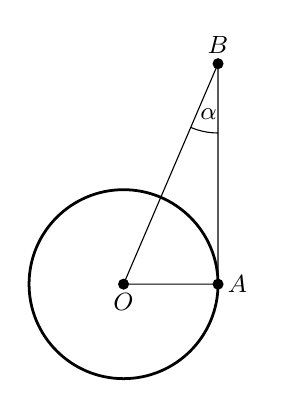
\begin{tikzpicture}[scale=0.8,every node/.style={font=\small}]
 \draw [line width=1pt] (0,0) circle (1.5);
 \draw (0,0) -- (1.5,0) -- (1.5,3.5) -- cycle;
 \fill (0,0) circle (2.5pt);
 \node [below] at (0,0) {$O$};
 \fill (1.5,0) circle (2.5pt);
 \node [right] at (1.5,0) {$A$};
 \fill (1.5,3.5) circle (2.5pt);
 \node [above] at (1.5,3.5) {$B$};
 \node at (1.35,2.7) {$\alpha$};
 \draw (1.5,2.4) arc (270:246.8:1.1);
\end{tikzpicture}}
%\picskip{12}
\noindent As another application of trigonometry to astronomy, we will find the distance from the earth
 to the sun. Let $O$ be the center of the earth, let $A$ be a point on the equator, and let $B$
 represent an object (e.g. a star) in space, as in the picture on the right. If the earth is
 positioned in such a way that the angle $\angle\,OAB = 90\Degrees$, then we say that the angle
 $\alpha = \angle\,OBA$ is the \emph{equatorial parallax}\index{equatorial parallax} of the object.
 The equatorial parallax of the sun has been observed to be approximately $\alpha =
 0.00244\Degrees$. Use this to estimate the distance from the center of the earth to the
 sun.\index{distance from earth to sun}\vspace{1mm}
 \par\noindent\textbf{Solution:} Let $B$ be the position of the sun. We want to find the length of
 $\overline{OB}$. We will use the actual radius of the earth, mentioned at the end of
 Example \ref{exmp:radearth}, to get $OA = 3956.6$ miles. Since $\angle\,OAB = 90\Degrees$, we have
 \begin{displaymath}
  \frac{OA}{OB} ~=~ \sin\;\alpha \quad\Rightarrow\quad OB ~=~ \frac{OA}{\sin\;\alpha} ~=~
   \frac{3956.6}{\sin\;0.00244\Degrees} ~=~ 92908394 ~,
 \end{displaymath}%%\picskip{0}\vspace{-21mm}
 so the distance from the center of the earth to the sun is approximately
 \fbox{$93$ million miles}~.\\Note: The
 earth's orbit around the sun is an ellipse, so the actual distance to the sun varies.
\end{exmp}\vspace{-3mm}
\divider
\vspace{1mm}

In the above example we used a very small angle ($0.00244\Degrees$). A degree can be divided into
smaller units: a \textbf{minute}\index{minute} is one-sixtieth of a degree, and a
\textbf{second}\index{second} is one-sixtieth of a minute. The symbol for a minute is $'$ and the
symbol for a second is $''$. For example, $4.5\Degrees = 4\Degrees\;30'$. And
$4.505\Degrees = 4\Degrees\;30'\;18''$:
\begin{displaymath}
 4\Degrees\;30'\;18'' ~=~ 4 ~+~ \frac{30}{60} ~+~ \frac{18}{3600} ~\text{degrees} ~=~ 4.505\Degrees
\end{displaymath}
In Example \ref{exmp:distsun} we used $\alpha = 0.00244\Degrees \approx 8.8''$, which we mention
only because some angle measurement devices do use minutes and seconds.\vspace{-2mm}

\begin{exmp}\label{exmp:radsun}
\parpic[r]{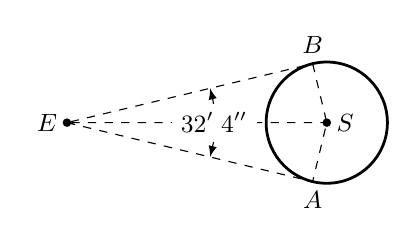
\begin{tikzpicture}[scale=1.1,every node/.style={font=\small}]
 \draw [line width=1pt] (3,0) circle (0.7);
 \fill (0,0) circle (1.4pt);
 \node [left] at (0,0) {$E$};
 \fill (3,0) circle (1.4pt);
 \node [right] at (3,0) {$S$};
 \draw [dashed] (0,0) -- ([shift={(3,0)}] 256.507:0.7) -- (3,0) -- ([shift={(3,0)}] 103.493:0.7)
  -- (0,0) -- (3,0);
 \node [below] at ([shift={(3,0)}] 256.507:0.7) {$A$};
 \node [above] at ([shift={(3,0)}] 103.493:0.7) {$B$};
 \draw [latex-latex] (-13.493:1.7) arc (-13.493:13.493:1.7);
 \node [fill=white] at (1.7,0) {$32'\;4''$};
\end{tikzpicture}}
\noindent An observer on earth measures an angle of $32'\;4''$ from one visible edge of the sun to the other
 (opposite) edge, as in the picture on the right. Use this to estimate the radius of the
 sun.\vspace{1mm}
 \par\noindent\textbf{Solution:} Let the point $E$ be the earth and let $S$ be the center of the sun.
 The observer's lines of sight to the visible edges of the sun are tangent lines to the sun's
 surface at
 the points $A$ and $B$. Thus, $\angle\,EAS = \angle\,EBS = 90\Degrees$. The radius of the sun
 equals $AS$. Clearly $AS = BS$. So since $EB = EA$ (why?), the triangles
 $\triangle\,EAS$ and $\triangle\,EBS$ are similar. Thus, $\angle\,AES = \angle\,BES = \frac{1}{2}\;
 \angle\,AEB = \frac{1}{2}\;(32'\;4'') = 16'\;2'' = (16/60) + (2/3600) = 0.26722\Degrees$.

 Now, $ES$ is the distance from the \emph{surface} of the earth (where the observer stands) to the
 center of the sun. In Example \ref{exmp:distsun} we found the distance from the \emph{center} of
 the earth to the sun to be $92,908,394$ miles. Since we treated the sun in that example as a point,
 then we are justified in treating that distance as the distance between the centers of the earth
 and sun. So $ES = 92908394 - ~\text{radius of earth} = 92908394 - 3956.6 = 92904437.4$ miles.
 Hence,
 \begin{displaymath}
  \sin\;(\angle\,AES) ~=~ \frac{AS}{ES} \quad\Rightarrow\quad AS ~=~ ES \;\sin\;0.26722\Degrees
  ~=~ (92904437.4)\;\sin\;0.26722\Degrees ~=~ \boxed{433,293 ~\text{miles}} ~.
 \end{displaymath}
 Note: This answer is close to the sun's actual (mean) radius of $432,200$ miles.\index{radius
 of sun}
\end{exmp}\vspace{-4mm}
\divider\vspace{-2mm}
\newpage
You may have noticed that the solutions to the examples we have shown required at least one right
triangle. In applied problems it is not always obvious which right triangle to use, which is why
these sorts of problems can be difficult. Often no right triangle will be immediately evident, so
you will have to create one. There is no general strategy for this, but remember that a right
triangle requires a right angle, so look for places where you can form perpendicular line segments.
When the problem contains a circle, you can create right angles by using the perpendicularity of
the tangent line\index{tangent line} to the circle at a point\footnote{This will often be worded as
\emph{the line that is tangent to the circle}.} with the line that joins that point to the center of
the circle. We did exactly that in Examples \ref{exmp:radearth}, \ref{exmp:distsun}, and
\ref{exmp:radsun}.

\vspace{2mm}
\begin{exmp}
\parpic[r]{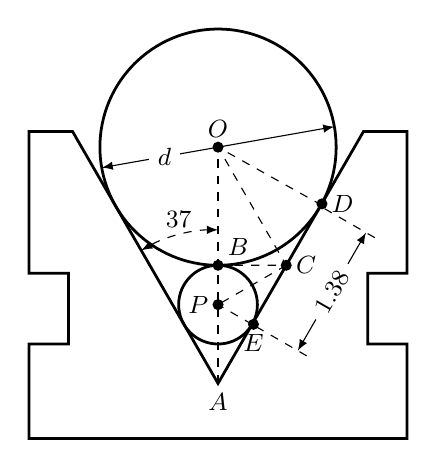
\begin{tikzpicture}[every node/.style={font=\small}]
 \draw [line width=1pt] (0,0) circle (1.5);
 \fill (0,0) circle (2pt);
 \node [above] at (0,0) {$O$};
 \draw [line width=1pt] (0,-2) circle (0.5);
 \fill (0,-2) circle (2pt);
 \node [left] at (0,-2) {$P$};
 \fill (0,-1.5) circle (2pt);
 \node [above right] at (0,-1.5) {$B$};
 \draw [dashed] (0,-3) -- (0,0);
 \draw [line width=1pt] (0,-3) -- (1.848,0.2) -- (2.4,0.2) -- (2.4,-1.6) -- (1.9,-1.6) --
  (1.9,-2.5) -- (2.4,-2.5) -- (2.4,-3.7) -- (-2.4,-3.7) -- (-2.4,-2.5) -- (-1.9,-2.5) --
  (-1.9,-1.6) -- (-2.4,-1.6) -- (-2.4,0.2) -- (-1.848,0.2) --cycle;
 \draw [latex-latex] (190:1.5) -- (10:1.5) node[fill=white,pos=0.27] {$d$};
 \draw [dashed] (1.32,-0.7379) -- (0,0) -- (0.866,-1.5) -- (0,-1.5);
 \draw [dashed] (0.866,-1.5) -- (0,-2);
 \draw [dashed] (0.433,-2.25) -- (0,-2);
 \node [right] at (0.866,-1.5) {$C$};
 \node [right] at (1.32,-0.72) {$D$};
 \node [below] at (0.45,-2.25) {$E$};
 \draw [rotate around={60:(0,-3)},latex-latex] (0.866,-3.67) -- (2.598,-3.67)
  node[fill=white,pos=0.5,rotate=60] {$1.38$};
 \draw [rotate around={60:(0,-3)},dashed] (0.866,-3.8) -- (0.866,-3);
 \draw [rotate around={60:(0,-3)},dashed] (2.598,-3.8) -- (2.598,-3);
 \draw [dashed,latex-latex] ([shift={(0,-3)}] 0,1.95) arc (90:120:1.95);
 \node[above] at (-0.5,-1.15) {$37\Degrees$};
 \node[below] at (0,-3) {$A$};
 \fill (0.866,-1.5) circle (2pt);
 \fill (1.32,-0.72) circle (2pt);
 \fill (0.45,-2.25) circle (2pt);
\end{tikzpicture}}
\noindent The machine tool diagram on the right shows a symmetric \emph{V-block}\index{v-block}, in which one
 circular roller sits on top of a smaller circular roller. Each roller touches both slanted sides of
 the V-block. Find the diameter $d$ of the large roller, given the information in the
 diagram.\vspace{1mm}
 \par\noindent\textbf{Solution:} The diameter $d$ of the large roller is twice the radius $OB$, so we
 need to find $OB$. To do this, we will show that $\triangle\,OBC$ is a right triangle, then find
 the angle $\angle\,BOC$, and then find $BC$. The length $OB$ will then be simple to determine.

 Since the slanted sides are tangent to each roller, $\angle\,ODA = \angle\,PEC =
 90\Degrees$. By symmetry, since the vertical line through the centers of the rollers makes a
 $37\Degrees$ angle with each slanted side, we have $\angle\,OAD = 37\Degrees$. Hence, since
 $\triangle\,ODA$ is a right triangle, $\angle\,DOA$ is the complement of $\angle\,OAD$. So
 $\angle\,DOA = 53\Degrees$.

 Since the horizontal line segment $\overline{BC}$ is tangent to each roller, $\angle\,OBC =
 \angle\,PBC = 90\Degrees$. Thus,
 $\triangle\,OBC$ is a right triangle. And since $\angle\,ODA = 90\Degrees$, we know that
 $\triangle\,ODC$ is a right triangle. Now, $OB = OD$ (since they each equal the radius of the large
 roller), so by the Pythagorean Theorem we have $BC = DC$:
 \begin{displaymath}
  BC^2 ~=~ OC^2 ~-~ OB^2 ~=~ OC^2 ~-~ OD^2 ~=~ DC^2 \quad\Rightarrow\quad BC ~=~ DC
 \end{displaymath}
 Thus, $\triangle\,OBC$ and $\triangle\,ODC$ are \emph{congruent triangles}\index{congruent
 triangles} (which we denote by $\triangle\,OBC \cong \triangle\,ODC$), since their corresponding
 sides are equal. Thus, their corresponding angles are equal. So in particular, $\angle\,BOC =
 \angle\,DOC$. We know that $\angle\,DOB = \angle\,DOA = 53\Degrees$. Thus,
 \begin{displaymath}
  53\Degrees ~=~ \angle\,DOB ~=~ \angle\,BOC ~+~ \angle\,DOC = \angle\,BOC ~+~ \angle\,BOC ~=~
  2\;\angle\,BOC \quad\Rightarrow\quad \angle\,BOC ~=~ 26.5\Degrees ~.
 \end{displaymath}
 Likewise, since $BP = EP$ and $\angle\,PBC = \angle\,PEC = 90\Degrees$, $\triangle\,BPC$ and
 $\triangle\,EPC$ are congruent right triangles. Thus, $BC = EC$. But we know that
 $BC = DC$, and we see from the diagram that $EC + DC = 1.38$. Thus, $BC + BC = 1.38$ and so
 $BC = 0.69$. We now have all we need to find $OB$:
 \begin{displaymath}
  \frac{BC}{OB} ~=~ \tan\;\angle\,BOC \quad\Rightarrow\quad OB ~=~ \frac{BC}{\tan\;\angle\,BOC} ~=~
  \frac{0.69}{\tan\;26.5\Degrees} ~=~ 1.384
 \end{displaymath}
 Hence, the diameter of the large roller is $\,d = 2 \times OB = 2\,(1.384) = \boxed{2.768}$~.
\end{exmp}
\divider
\newpage
\begin{exmp}\label{exmp:crank}
 A \emph{slider-crank mechanism}\index{slider-crank mechanism} is shown in Figure \ref{fig:crank}
 below. As the piston moves downward the connecting rod rotates the crank in the clockwise
 direction, as indicated.

 \begin{figure}[h]
 \begin{center}
  \begin{tikzpicture}[every node/.style={font=\small}]
  \draw [dashed] (0,-7.5) circle (2.5);
  \filldraw [fill=white,line width=1pt,rounded corners,rotate around={15.255:(0,0)}] (240:0.9)
   arc (240:-60:0.9) -- ([shift={(0,-5.7)}] 37.875:1.1) arc (37.875:-217.875:1.1) -- cycle;
  \filldraw [fill=white,line width=1pt,rotate around={53.13:(0,-7.5)}] (0,-6.6) -- (2.5,-6.6) arc
   (90:-90:0.9) -- (0,-8.4) arc (270:90:0.9);
  \draw[dashed] (0,0) -- (1.5,-5.5) node[black,pos=0.55,sloped,below] {connecting rod}
   node[midway,above right] {$b$};
  \draw [line width=1pt] (0,0) circle (0.6);
  \fill (0,0) circle (2pt);
  \node [above] at (0,0) {$A$};
  \draw [line width=1pt] (1.5,-5.5) circle (0.6);
  \fill (1.5,-5.5) circle (2pt);
  \node [below] at (1.5,-5.5) {$B$};
  \draw [line width=1pt] (0,-7.5) circle (0.6);
  \fill (0,-7.5) circle (2pt);
  \node [below] at (0,-7.5) {$O$};
  \draw [dashed] (0,-7.5) -- (1.5,-5.5) node[sloped,midway,below] {crank};
  \draw [dashed] (0,0) -- (5.625,0) node[above,pos=0.7] {$a$};
  \draw [dashed] (1.5,-5.5) -- (5.625,0) node[midway,right] {$c$};
  \fill (5.625,0) circle (2pt);
  \node [right] at (5.625,0) {$C$};
  \draw [dashed,latex-latex] (-2.5,-7.5) -- (-0.05,-7.5) node[pos=0.4,fill=white] {$r$};
  \draw [dashed] (0,-7.5) -- (0,0);
  \draw [dashed,-latex] (0,-6.4) arc (90:53.13:1.1);
  \node at (0.4,-6.25) {$\theta$};
  \draw [line width=1pt] (-1.3,1.2) -- (1.3,1.2) -- (1.3,-1) -- (1.7,-1) -- (1.7,2) -- (-1.7,2) --
   (-1.7,-1) -- (-1.3,-1) -- cycle;
  \node at (0,1.6) {piston};
  \pattern[pattern color=black,pattern=north east lines] (-2,2.4) -- (-1.8,2.4) -- (-1.8,-1.4)
   -- (-2,-1.4) -- cycle;
  \draw [line width=1pt] (-1.8,2.4) -- (-1.8,-1.4);
  \pattern[pattern color=black,pattern=north east lines] (2,2.4) -- (1.8,2.4) -- (1.8,-1.4)
   -- (2,-1.4) -- cycle;
  \draw [line width=1pt] (1.8,2.4) -- (1.8,-1.4);
  \draw [linecolor,line width=1.5pt,-latex] (0,2.6) -- (0,2.1);
  \draw [linecolor,line width=1.5pt,-latex] (2.7,-7.5) arc (360:330:2.7);
 \end{tikzpicture} \vspace{-5mm}
 \end{center}
 \caption[]{\quad Slider-crank mechanism}
 \label{fig:crank}
\end{figure}

The point $A$ is the center of the connecting rod's \emph{wrist pin} and only moves vertically.
The point $B$ is the center of the \emph{crank pin} and moves around a circle of radius $r$ centered
at the point $O$, which is directly below $A$ and does not move. As the crank rotates it makes an
angle $\theta$ with the line $\overline{OA}$.
The \emph{instantaneous center of rotation}\index{instantaneous center of rotation} of the
connecting rod at a given time is the point $C$ where the horizontal line through $A$ intersects the
extended line through $O$ and $B$.
From Figure \ref{fig:crank} we see that $\angle\,OAC = 90\Degrees$, and we let
$a = AC$, $b = AB$, and $c = BC$. In the exercises you will show that for
$0\Degrees < \theta < 90\Degrees$,
\begin{displaymath}
 c ~=~ \frac{\sqrt{b^2 ~-~ r^2 \;(\sin \theta)^2}}{\cos\;\theta} ~\qquad\text{and}\qquad~
 a ~=~ r\;\sin\;\theta ~+~ \sqrt{b^2 ~-~ r^2 \;(\sin \theta)^2}~\tan\;\theta ~.
\end{displaymath}
\end{exmp}
\divider
\newpage
\parpic[r]{\begin{tikzpicture}[scale=0.5,every node/.style={font=\small}]
   \fill [fill=fillcolor] (0,0) -- (4,0) -- (4,3) -- (0,0);
   \node at (1.05,0.38) {$\theta$};
   \draw (1.5,0) arc (0:37:1.5);
   \draw [line width=0.5pt] (3.6,0) -- (3.6,0.4) -- (4,0.4);
   \draw [linecolor,line width=1.5pt] (0,0) -- (4,0) -- (4,3) -- cycle;
   \node [below] at (2,0) {$r\;\cos\;\theta$};
   \node [right] at (4,1.5) {$r\;\sin\;\theta$};
   \node [above left] at (2,1.5) {$r$};
  \end{tikzpicture}}
For some problems it may help to remember that when a right triangle has a hypotenuse of length $r$
and an acute angle $\theta$, as in the picture on the right, the adjacent side will have length
$r\,\cos\;\theta$ and the opposite side will have length $r\,\sin\;\theta$. You can think of those
lengths as the horizontal and vertical ``components'' of the hypotenuse.

Notice in the above right triangle that we were given two pieces of information: one of the acute
angles and the length of the hypotenuse. From this we determined the lengths of the other two
sides, and the other acute angle is just the complement of the known acute angle. In general, a
triangle has six parts: three sides and three angles. \textbf{Solving a triangle}\index{solving a
triangle} means finding the unknown parts based on the known parts. In the case of a right triangle,
one part is always known: one of the angles is $90\Degrees$.

\begin{exmp}
\piccaption[]{\label{fig:solveright}}\parpic[r]{\begin{tikzpicture}[scale=0.4,
 every node/.style={font=\small}]
 \fill [fill=fillcolor] (0,0) -- (4,0) -- (4,3) -- (0,0);
 \draw [line width=0.5pt] (3.6,0) -- (3.6,0.4) -- (4,0.4);
 \draw [linecolor,line width=1.5pt] (0,0) -- (4,0) -- (4,3) -- cycle;
 \node [below left] at (0,0) {$A$};
 \node [below right] at (4,0) {$C$};
 \node [above right] at (4,3) {$B$};
 \node [below] at (2,0) {$b$};
 \node [right] at (4,1.5) {$a$};
 \node [above left] at (2,1.5) {$c$};
\end{tikzpicture}}
\noindent Solve the right triangle in Figure \ref{fig:solveright} using the given\\information:
 \begin{enumerate}[\bfseries (a)]
  \item $c = 10$, $A = 22\Degrees$
   \par\noindent\textbf{Solution:} The unknown parts are $a$, $b$, and $B$. Solving yields:
   \begin{alignat*}{7}
    a ~ &= ~ c\;\sin\;A ~ &= ~ 10\;\sin\;22\Degrees ~ &= ~ 3.75\\
    b ~ &= ~ c\;\cos\;A ~ &= ~ 10\;\cos\;22\Degrees ~ &= ~ 9.27\\
    B ~ &= ~ 90\Degrees ~-~ A ~ &= ~ 90\Degrees ~-~ 22\Degrees ~ &= ~ 68\Degrees
   \end{alignat*}
  \item $b = 8$, $A = 40\Degrees$
   \par\noindent\textbf{Solution:} The unknown parts are $a$, $c$, and $B$. Solving yields:
   \begin{alignat*}{3}
    \frac{a}{b} ~ &= ~ \tan\;A \quad &\Rightarrow \quad a ~ &= ~ b\;\tan\;A ~ = ~
	 8\;\tan\;40\Degrees ~ = ~ 6.71\\[2mm]
    \frac{b}{c} ~ &= ~ \cos\;A \quad &\Rightarrow \quad c ~ &= ~ \frac{b}{\cos\;A} ~ = ~
	 \frac{8}{\cos\;40\Degrees} ~ = ~ 10.44
   \end{alignat*}
   \begin{displaymath}
    B ~ = ~ 90\Degrees ~-~ A ~ = ~ 90\Degrees ~-~ 40\Degrees ~ = ~ 50\Degrees
   \end{displaymath}
  \item $a = 3$, $b = 4$
   \par\noindent\textbf{Solution:} The unknown parts are $c$, $A$, and $B$. By the Pythagorean
   Theorem,
   \begin{displaymath}
    c ~=~ \sqrt{a^2 ~+~ b^2} ~=~ \sqrt{3^2 ~+~ 4^2} ~=~ \sqrt{25} ~=~ 5 ~.
   \end{displaymath}
   Now, $\tan\;A = \frac{a}{b} = \frac{3}{4} = 0.75$. So how do we find $A$?
   There should be a key labeled {\setlength\fboxsep{1pt}\ovalbox{\footnotesize $\tan^{-1}$}}
   on your calculator, which works like
   this: give it a number $x$ and it will tell you the angle $\theta$ such that $\tan\;\theta = x$.
   In our case, we want the angle $A$ such that $\tan\;A = 0.75$:
   \begin{displaymath}
    \text{Enter: } 0.75 \quad \text{Press:
	{\setlength\fboxsep{1pt}\ovalbox{\footnotesize $\tan^{-1}$}}} \quad \text{Answer: } 36.86989765
   \end{displaymath}
   This tells us that $A = 36.87\Degrees$, approximately. Thus $B = 90\Degrees - A = 
   90\Degrees - 36.87\Degrees = 53.13\Degrees$.\\Note: The
   {\setlength\fboxsep{1pt}\ovalbox{\footnotesize $\sin^{-1}$}} and
   {\setlength\fboxsep{1pt}\ovalbox{\footnotesize $\cos^{-1}$}}
   keys work similarly for sine and cosine, respectively. These keys
   use the \emph{inverse trigonometric functions}\index{inverse trigonometric functions}, which we
   will discuss in Chapter 5.
 \end{enumerate}
\end{exmp}\vspace{-2mm}
\divider

\newpage
\startexercises\label{sec1dot3}
\vspace{4mm}
{\small
\begin{enumerate}[\bfseries 1.]
\parpic[r]{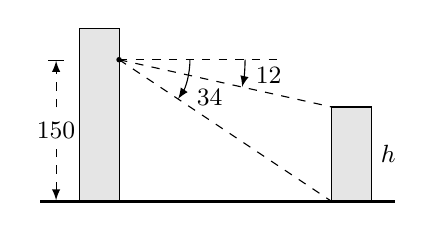
\begin{tikzpicture}[every node/.style={font=\small}]
 \begin{scope}[>=latex]
  \draw [dashed,|<->|] (-0.8,0) -- (-0.8,1.8) node [midway,fill=white] {$150$};
 \end{scope}
 \draw [fill=black!10] (-0.5,0) -- (-0.5,2.2) -- (0,2.2) -- (0,0);
 \fill (0,1.8) circle (1pt);
 \draw [fill=black!10] (2.7,0) -- (2.7,1.2) -- (3.2,1.2) -- (3.2,0);
 \draw [line width=1pt] (-1,0) -- (3.5,0);
 \node [right] at (3.2,0.6) {$h$};
 \draw [dashed] (0,1.8) -- (2,1.8);
 \draw [dashed] (0,1.8) -- (2.7,1.2);
 \draw [dashed] (0,1.8) -- (2.7,0);
 \draw [-latex] ([shift={(0,1.8)}] 1.6,0) arc (0:-12.53:1.6);
 \node at (1.9,1.6) {$12\Degrees$};
 \draw [-latex] ([shift={(0,1.8)}] 0.9,0) arc (0:-33.69:0.9);
 \node at (1.15,1.32) {$34\Degrees$};
\end{tikzpicture}}
 \item From a position $150$ ft above the ground, an observer in a building measures angles of
 depression of $12\Degrees$ and $34\Degrees$ to the top and bottom, respectively, of a smaller
 building, as in the picture on the right. Use this to find the height $h$ of the smaller
 building.\vspace{4mm}
\suspend{enumerate}
\resume{enumerate}[{[\bfseries 1.]}]
\parpic[r]{\begin{tikzpicture}[scale=1.0,every node/.style={font=\small}]
 \fill [brickcolor] (2.7,0) -- (2.9,0.7) -- (3,0.7) -- (3.2,1.4) -- (3.3,1.4) --
  (3.5,2) -- (4,1.2) -- (4.2,1.2) -- (4.5,0);
 \draw [dashed] (3.5,0) -- (3.5,2) node [pos=0.4,right] {$h$};
 \draw [dashed] (0,0) -- (3.5,2.06);
 \draw [dashed] (1.5,0) -- (3.5,2.06);
 \draw (3.3,0) -- (3.3,0.2) -- (3.5,0.2);
 \draw [line width=2pt] (2.7,0) -- (2.9,0.7) -- (3,0.7) -- (3.2,1.4) -- (3.3,1.4) --
  (3.5,2) -- (4,1.2) -- (4.2,1.2) -- (4.5,0);
 \begin{scope}[>=latex]
  \draw [|<->|] (0,-0.2) -- (1.5,-0.2) node [midway,fill=white] {$b$};
  \draw [<->|] (1.5,-0.2) -- (2.7,-0.2) node [midway,fill=white] {$a$};
 \end{scope}
 \draw (0,0) -- (4.5,0);
 \node [above right] at (0.48,-0.07) {$\beta$};
 \draw [dashed] (1.1,0) arc (0:29.8:1.1);
 \node [above right] at (1.7,-0.05) {$\alpha$};
 \draw [dashed] (2.3,0) arc (0:45.4:0.8);
\end{tikzpicture}}
 \item Generalize Example \ref{exmp:mountain}: A person standing $a$ ft from the base of a
 mountain measures an angle of elevation $\alpha$ from the ground to the top of the mountain.
 The person then walks $b$ ft straight back and measures an angle of elevation $\beta$ to the top
 of the mountain, as in the picture on the right. Assuming the ground is level, find a formula for
 the height $h$ of the mountain in terms of $a$, $b$, $\alpha$, and $\beta$.
\suspend{enumerate}
\resume{enumerate}[{[\bfseries 1.]}]
 \item As the angle of elevation from the top of a tower to the sun decreases from $64\Degrees$ to
 $49\Degrees$ during the day, the length of the shadow of the tower increases by $92$ ft along the
 ground. Assuming the ground is level, find the height of the tower.\vspace{2mm}
\parpic[r]{\begin{tikzpicture}[every node/.style={font=\small}]
 \fill [watercolor] (-0.7,0) -- (3.7,0) -- (3.7,1.5) -- (-0.7,1.5) -- cycle;
 \pattern[pattern color=white,pattern=horizontal lines] (-0.7,0) -- (3.7,0) --
  (3.7,1.5) -- (-0.7,1.5) -- cycle;
 \draw [line width=1pt] (-0.7,0) -- (3.7,0);
 \draw [line width=1pt] (-0.7,1.5) -- (3.7,1.5);
 \fill (0,1.5) circle (2pt);
 \node [above] at (0,1.5) {$A$};
 \fill (2.7,1.5) circle (2pt);
 \node [above] at (2.7,1.5) {$B$};
 \fill (1,0) circle (2pt);
 \node [below] at (1,0) {$C$};
 \node [above] at (1.35,1.5) {$500$};
 \draw [latex-latex] (3.2,0) -- (3.2,1.5) node[midway,right] {$w$};
 \draw [dashed] (0,1.5) -- (1,0) -- (2.7,1.5);
 \draw [dashed] ([shift={(0,1.5)}] 0.9,0) arc (0:-56.3:0.9);
 \node at (0.6,1.32) {$56\Degrees$};
 \draw [dashed] ([shift={(2.7,1.5)}] -0.9,0) arc (180:221.42:0.9);
 \node at (2.2,1.32) {$41\Degrees$};
\end{tikzpicture}}
 \item Two banks of a river are parallel, and the distance between two points $A$ and $B$ along
 one bank is $500$ ft. For a point $C$ on the opposite bank, $\angle\,BAC = 56\Degrees$ and
 $\angle\,ABC = 41\Degrees$, as in the picture on the right. What is the width $w$ of the
 river?\\(\emph{Hint: Divide $\overline{AB}$ into two pieces.})\vspace{5mm}
\suspend{enumerate}
\resume{enumerate}[{[\bfseries 1.]}]
\parpic[r]{\begin{tikzpicture}[every node/.style={font=\small}]
 \fill [watercolor] (0,0) -- (5,0) -- (5,1) -- (0,1) -- cycle;
 \pattern[pattern color=white,pattern=horizontal lines] (0,0) -- (5,0) --
  (5,1) -- (0,1) -- cycle;
 \draw [line width=1pt] (0,0) -- (5,0);
 \draw [line width=1pt] (0,1) -- (5,1);
 \fill (0.2,-1) circle (2pt);
 \node [below] at (0.2,-1) {$A$};
 \fill (4.5,-0.7) circle (2pt);
 \node [below] at (4.5,-0.7) {$B$};
 \fill [fill=black!10] (2.8,3) arc (0:180:0.3 and 0.2) -- (2.2,3) arc (180:360:0.3 and 0.2);
 \shadedraw [left color=black!40,right color=black!40,middle color=black!10] (2.2,1.7)
  arc (180:360:0.3 and 0.2) -- (2.8,3) -- (2.8,3) arc (360:180:0.3 and 0.2) -- (2.2,1.7);
 \draw (2.8,3) arc (0:180:0.3 and 0.2);
 \draw [dashed] (2.5,1.5) -- (0.2,-1);
 \draw [dashed] (2.5,1.5) -- (4.5,-0.7);
 \draw [dashed] (2.5,2.8) -- (0.2,-1);
 \draw [dashed] (2.5,2.8) -- (4.5,-0.7);
 \draw [dashed] (2.5,2.8) -- (2.5,1.5);
 \draw [dashed] (0.2,-1) -- (4.5,-0.7) node[midway,below] {$d$};
 \draw [rotate around={-45:(2.5,1.5)}] (2.7,1.5) -- (2.7,1.3) -- (2.5,1.3);
 \draw [rotate around={135:(4,2)},-latex] (4,2) -- (4.5,2) node [above] {N};
 \draw [rotate around={45:(4,2)},-latex] (4,2) -- (4.5,2) node [above] {E};
 \node at (3.4,0.77) {$\beta$};
 \node at (1.3,0.45) {$\alpha$};
 \draw [rotate around={47.2:(0.2,-1)}] ([shift={(0.2,-1)}] 1.65,0) arc (0:11.8:1.65);
 \draw [rotate around={119.6:(4.5,-0.7)}] ([shift={(4.5,-0.7)}] 1.65,0) arc (0:12.4:1.65);
 \draw [dashed] (1,2.8) -- (2.5,2.8);
 \draw [dashed] (1,1.5) -- (2.5,1.5);
 \draw [latex-latex] (1.2,1.5) -- (1.2,2.8) node [midway,fill=white] {$h$};
\end{tikzpicture}}
 \item A tower on one side of a river is directly east and north of points $A$ and $B$,
 respectively, on the other side of the river. The top of the tower has angles of elevation $\alpha$
 and $\beta$ from $A$ and $B$, respectively, as in the picture on the right. Let $d$ be the distance
 between $A$ and $B$. Assuming that both sides of the river are at the same elevation, show that the
 height $h$ of the tower is
 \begin{displaymath}
  h ~=~ \frac{d}{\sqrt{\cot^2 \,\alpha ~+~ \cot^2 \,\beta}} ~.
 \end{displaymath}\vspace{1mm}
\suspend{enumerate}
\resume{enumerate}[{[\bfseries 1.]}]
\item\label{exer:distmoon} The equatorial parallax of the moon has been observed to be approximately
$57'$. Taking the radius of the earth to be $3956.6$ miles, estimate the distance from the center of
the earth to the moon. (\emph{Hint: See Example \ref{exmp:distsun}.})
\item An observer on earth measures an angle of $31'\;7''$ from one visible edge of the moon to the
other (opposite) edge. Use this to estimate the radius of the moon. (\emph{Hint: Use Exercise
\ref{exer:distmoon} and see Example \ref{exmp:radsun}.})
\newpage
\parpic[r]{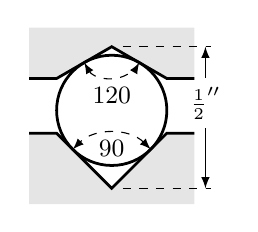
\begin{tikzpicture}[scale=0.7,every node/.style={font=\small}]
 \draw [latex-latex] (1.7,-1.414) -- (1.7,1.1547) node[pos=0.6,fill=white] {$\frac{1}{2}''$};
 \fill [black!10] (-1.5,-0.414) -- (-1,-0.414) --
  (0,-1.414) -- (1,-0.414) -- (1.5,-0.414) -- (1.5,-1.7) -- (-1.5,-1.7) -- cycle;
% \pattern[pattern color=white,pattern=north east lines] (-1.5,-0.414) -- (-1,-0.414) --
%  (0,-1.414) -- (1,-0.414) -- (1.5,-0.414) -- (1.5,-1.7) -- (-1.5,-1.7) -- cycle;
 \draw [line width=1pt] (-1.5,-0.414) -- (-1,-0.414) -- (0,-1.414) -- (1,-0.414) -- (1.5,-0.414);
 \fill [black!10] (-1.5,0.5777) -- (-1,0.5777) --
  (0,1.1547) -- (1,0.5777) -- (1.5,0.5777) -- (1.5,1.5) -- (-1.5,1.5) -- cycle;
% \pattern[pattern color=white,pattern=north east lines]  (-1.5,0.5777) -- (-1,0.5777) --
%  (0,1.1547) -- (1,0.5777) -- (1.5,0.5777) -- (1.5,1.5) -- (-1.5,1.5) -- cycle;
 \draw [line width=1pt] (-1.5,0.5777) -- (-1,0.5777) -- (0,1.1547) -- (1,0.5777) -- (1.5,0.5777);
 \draw [line width=1pt] (0,0) circle (1);
 \draw [dashed,line width=0.5pt] (0.2,1.1547) -- (1.8,1.1547);
 \draw [dashed,line width=0.5pt] (0.2,-1.414) -- (1.8,-1.414);
 \draw [dashed,latex-latex] ([shift={(0,-1.414)}] 45:1) arc (45:135:1);
 \node [below] at (0,-0.37) {$90\Degrees$};
 \draw [dashed,latex-latex] ([shift={(0,1.1547)}] 210:0.577) arc (210:330:0.577);
 \node [below] at (0,0.6) {$120\Degrees$};
\end{tikzpicture}}
\item A ball bearing sits between two metal grooves, with the top groove having an angle of
$120\Degrees$ and the bottom groove having an angle of $90\Degrees$, as in the picture on the right.
What must the diameter of the ball bearing be for the distance between the vertices of the
grooves to be half an inch? You may assume that the top vertex is directly above the bottom
vertex.\vspace{2mm}
\suspend{enumerate}
\resume{enumerate}[{[\bfseries 1.]}]
\parpic[r]{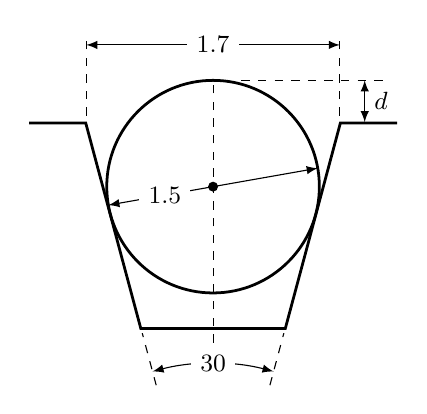
\begin{tikzpicture}[scale=1.8,every node/.style={font=\small}]
 \draw [line width=1pt] (0,0) circle (0.75);
 \draw [rotate=10,latex-latex] (-0.75,0) -- (0.75,0) node[pos=0.27,sloped,fill=white] {$1.5$};
 \fill (0,0) circle (1pt);
 \draw [line width=1pt] (0,-1) -- (0.51,-1) -- ++(75:1.5) -- ++(0.4,0);
 \draw [line width=1pt] (0,-1) -- (-0.51,-1) -- ++(105:1.5) -- ++(-0.4,0);
 \draw [dashed] (-0.895,0.5) -- (-0.895,1.08);
 \draw [dashed] (0.895,0.5) -- (0.895,1.08);
 \draw [latex-latex] (-0.895,1.0) -- (0.895,1.0) node[midway,fill=white] {$1.7$};
 \draw [dashed] (0.2,0.75) -- (1.25,0.75);
 \draw [latex-latex] (1.07,0.75) -- (1.07,0.455) node[midway,right] {$d$};
 \draw [dashed] ([shift={(0,-2.898)}] 75:1.55) -- ++(75:0.38);
 \draw [dashed] ([shift={(0,-2.898)}] 105:1.55) -- ++(105:0.38);
 \draw [dashed] (0,-1.1) -- (0,0.75);
 \draw [latex-latex] ([shift={(0,-2.898)}] 105:1.65) arc (105:75:1.65);
 \node [fill=white] at (0,-1.248) {$30\Degrees$};
\end{tikzpicture}}
\item\label{exer:worm} The machine tool diagram on the right shows a symmetric
\emph{worm thread}\index{worm thread},
in which a circular roller of diameter $1.5$ inches sits. Find the amount $d$ that the top of the
roller rises above the top of the thread, given the information in the diagram. (\emph{Hint: Extend
the slanted sides of the thread until they meet at a point.})
\item Repeat Exercise \ref{exer:worm} using $1.8$ inches as the distance across the top of the
worm thread.
\item In Exercise \ref{exer:worm}, what would the distance across the top of the worm thread have
to be to make $d$ equal to $0$ inches?
\suspend{enumerate}
\resume{enumerate}[{[\bfseries 1.]}]
\item For $0\Degrees < \theta < 90\Degrees$ in the slider-crank mechanism in Example
\ref{exmp:crank}, show that
\begin{displaymath}
 c ~=~ \frac{\sqrt{b^2 ~-~ r^2 \;\sin^2 \,\theta}}{\cos\;\theta} ~\qquad\text{and}\qquad~
 a ~=~ r\;\sin\;\theta ~+~ \sqrt{b^2 ~-~ r^2 \;\sin^2 \,\theta}~\tan\;\theta ~.
\end{displaymath}
\par\noindent (\emph{Hint: In Figure \ref{fig:crank} draw line segments from $B$ perpendicular to
$\overline{OA}$ and $\overline{AC}$.})
\parpic[r]{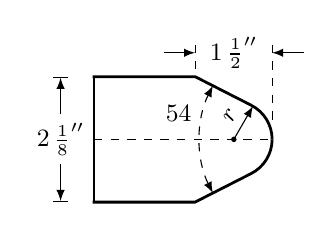
\begin{tikzpicture}[every node/.style={font=\small}]
 \draw [line width=1pt] (0.4866,0) arc (0:63:0.4866) -- ++(153:0.8) -- ++(-1.3,0);
 \draw [line width=1pt] (0.4866,0) arc (0:-63:0.4866) -- ++(-153:0.8) -- ++(-1.3,0);
 \fill (0,0) circle (1pt);
 \draw [-latex] (0,0) -- (60:0.4866) node[above,sloped,midway,above] {$r$};
 \begin{scope}[>=latex]
  \draw [|<->|] (-2.2,0.7964) -- (-2.2,-0.7964) node [midway,fill=white] {$2\,\frac{1}{8}''$};
 \end{scope}
 \draw [line width=1pt] (-1.775,0.7964) -- (-1.775,-0.7964);
 \draw [dashed] (-1.775,0) -- (0.4866,0);
 \draw [dashed] (-0.492,1.2) -- (-0.492,0.9);
 \draw [dashed] (0.4866,1.2) -- (0.4866,0.2);
 \node at (-0.0027,1.1) {$1\,\frac{1}{2}''$};
 \draw [-latex] (-0.892,1.1) -- (-0.492,1.1);
 \draw [-latex] (0.8866,1.1) -- (0.4866,1.1);
 \draw [dashed,latex-latex] ([shift={(1.071,0)}] 153:1.5) arc (153:207:1.5);
 \node[above] at (-0.7,0.1) {$54\Degrees$};
\end{tikzpicture}}
\item The machine tool diagram on the right shows a symmetric
\emph{die punch}\index{die punch}. In this view, the rounded tip is part of a
circle of radius $r$, and the slanted sides are tangent to that circle and form an angle of
$54\Degrees$. The top and bottom sides of the die punch are horizontal. Use the
information in the diagram to find the radius $r$.\vspace{1mm}
\suspend{enumerate}
\resume{enumerate}[{[\bfseries 1.]}]
\parpic[r]{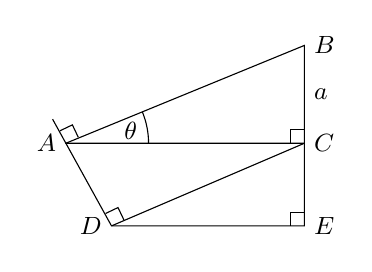
\begin{tikzpicture}[scale=0.7,every node/.style={font=\small}]
 \draw (0,0) -- (3.5,0) -- (3.5,3.275) -- (-0.828,1.5) -- cycle;
 \draw (0,0) -- (3.5,1.5);
 \draw (3.5,1.5) -- (-0.828,1.5) -- +(118.9:0.5);
 \node [left] at (-0.828,1.5) {$A$};
 \node [right] at (3.5,3.275) {$B$};
 \node [right] at (3.5,1.5) {$C$};
 \node [left] at (0,0) {$D$};
 \node [right] at (3.5,0) {$E$};
 \node [right] at (3.5,2.3875) {$a$};
 \node at (0.35,1.725) {$\theta$};
 \draw ([shift={(-0.828,1.5)}] 1.5,0) arc (0:22.3:1.5);
 \draw [shift={(-0.828,1.5)},rotate=25.5] (0.25,0) -- (0.25,0.25) -- (0,0.25);
 \draw [rotate=25.5] (0.25,0) -- (0.25,0.25) -- (0,0.25);
 \draw (3.25,0) -- (3.25,0.25) -- (3.5,0.25);
 \draw (3.25,1.5) -- (3.25,1.75) -- (3.5,1.75);
\end{tikzpicture}}
 \item In the figure on the right, $\angle\,BAC = \theta$ and $BC = a$. Use this to find
 $AB$, $AC$, $AD$, $DC$, $CE$, and $DE$ in terms of $\theta$ and $a$.\\(\emph{Hint: What
 is the angle $\angle\,ACD\,$?})\vspace{15mm}
\suspend{enumerate}
\piccaption[]{\label{fig:exersolveright}}\parpic[r]{\begin{tikzpicture}[scale=0.4,
 every node/.style={font=\small}]
 \fill [fill=fillcolor] (0,0) -- (4,0) -- (4,3) -- (0,0);
 \draw [line width=0.5pt] (3.5,0) -- (3.5,0.5) -- (4,0.5);
 \draw [linecolor,line width=1.5pt] (0,0) -- (4,0) -- (4,3) -- cycle;
 \node [below left] at (0.2,0) {$A$};
 \node [below right] at (3.8,0) {$C$};
 \node [above right] at (3.8,2.9) {$B$};
 \node [below] at (2,0) {$b$};
 \node [right] at (4,1.5) {$a$};
 \node [above left] at (2,1.5) {$c$};
\end{tikzpicture}}
\picskip{5}
\par\noindent For Exercises \ref{exer:solvrtfirst}-\ref{exer:solvrtlast}, solve the right triangle
in Figure \ref{fig:exersolveright} using the\\given information.
\resume{enumerate}[{[\bfseries 1.]}]
 \begin{multicols}{3}
  \item\label{exer:solvrtfirst} $a = 5$, $b = 12$
  \item $c = 6$, $B = 35\Degrees$
  \item $b = 2$, $A = 8\Degrees$
 \end{multicols}
 \begin{multicols}{3}
  \item $a = 2$, $c = 7$
  \item $a = 3$, $A = 26\Degrees$
  \item $b = 1$, $c = 2$
 \end{multicols}
 \begin{multicols}{3}
  \item $b = 3$, $B = 26\Degrees$
  \item $a = 2$, $B = 8\Degrees$
  \item\label{exer:solvrtlast} $c = 2$, $A = 45\Degrees$
 \end{multicols}
\suspend{enumerate}
\resume{enumerate}[{[\bfseries 1.]}]
 \item In Example \ref{exmp:funcs75} in Section 1.2, we found the exact values of all six
 trigonometric functions of $75\Degrees$. For example, we showed that $\cot\;75\Degrees =
 \frac{\sqrt{6} -
 \sqrt{2}}{\sqrt{6} + \sqrt{2}}$. So since $\tan\;15\Degrees = \cot\;75\Degrees$ by the Cofunction
 Theorem, this means that $\tan\;15\Degrees = \frac{\sqrt{6} - \sqrt{2}}{\sqrt{6} + \sqrt{2}}$. We
 will now describe another method for finding the exact values of the trigonometric functions of
 $15\Degrees$. In fact, it can be used to find the exact values for the trigonometric functions of
 $\frac{\theta}{2}$ when those for $\theta$ are known, for any $0\Degrees < \theta < 90\Degrees$.
 The method is illustrated in Figure \ref{fig:semicircles} and is described below.\vspace{2mm}

\piccaption[]{\label{fig:semicircles}}\parpic(\textwidth,0in){\begin{tikzpicture}[scale=1.7,
 every node/.style={font=\small}]
   \draw [black] (-6.5,0) -- (1.5,0);
   \draw [black] (1,0) arc (0:180:1);
   \fill (0,0) circle (1.3pt);
   \draw [black] (0,0) -- (60:1);
   \draw [dashed,black] (0.5,0) -- (60:1);
   \draw [black] (0.4,0) -- (0.4,0.1) -- (0.5,0.1);
   \fill [red] (-1,0) circle (1.3pt);
   \draw [red] (-1,0) -- (60:1);
   \draw [red] (0.732,0) arc (0:180:1.732);
   \fill [blue] (-2.732,0) circle (1.3pt);
   \draw [blue] (-2.732,0) -- (60:1);
   \draw [blue] (0.614,0) arc (0:180:3.346);
   \fill [green!85!black] (-6.078,0) circle (1.3pt);
   \draw [green!85!black] (-6.078,0) -- (60:1);
   \fill (60:1) circle (1.3pt);
   \node at (0.25,0.1) {$60\Degrees$};
   \node at (-0.55,0.1) {$30\Degrees$};
   \node at (-1.85,0.1) {$15\Degrees$};
   \node at (-4.5,0.1) {$7.5\Degrees$}; 
   \node [below] at (0,0) {$O$};
   \node [below] at (0.5,0) {$Q$};
   \node [below] at (1,0) {$1$};
   \node [below] at (-1,0) {$A$};
   \node [below] at (-2.732,0) {$B$};
   \node [below] at (-6.078,0) {$C$};
   \node [above right] at (60:1) {$P$};
  \end{tikzpicture}\piccaptioninside}
 \par\mbox{}\newline\vspace{1mm}\picskip{0}
Draw a semicircle of radius $1$ centered at a point $O$ on a horizontal line. Let $P$ be the point
on the semicircle such that $\overline{OP}$ makes an angle of $60\Degrees$ with the horizontal line,
as in Figure \ref{fig:semicircles}. Draw a line straight down from $P$ to the horizontal line at the
point $Q$.
Now create a second semicircle as follows: Let $A$ be the left endpoint of the first semicircle,
then draw a new semicircle centered at $A$ with radius equal to $AP$. Then create a third semicircle
in the same way: Let $B$ be the left endpoint of the second semicircle, then draw a new semicircle
centered at $B$ with radius equal to $BP$.\vspace{1.5mm}\\This procedure can be continued indefinitely
to create more semicircles. In general, it can be shown
that the line segment from the center of the new semicircle to $P$ makes an angle with the
horizontal line equal to half the angle from the previous semicircle's center to $P$.

 \begin{enumerate}[\bfseries (a)]
  \item Explain why $\angle\,PAQ=30\Degrees$. (\emph{Hint: What is the supplement of $60\Degrees$?})
  \item Explain why $\angle\,PBQ=15\Degrees$ and $\angle\,PCQ=7.5\Degrees$.
  \item Use Figure \ref{fig:semicircles} to find the exact values of $\sin\;15\Degrees$,
   $\cos\;15\Degrees$,
   and $\tan\;15\Degrees$. (\emph{Hint: To start, you will need to use $\angle\,POQ = 60\Degrees$
   and $OP = 1$ to find the exact lengths of $\overline{PQ}$ and $\overline{OQ}$.})
  \item Use Figure \ref{fig:semicircles} to calculate the exact value of $\tan\;7.5\Degrees$.
  \item Use the same method but with an initial angle of $\angle\,POQ = 45\Degrees$ to find the
   exact values of $\sin\;22.5\Degrees$, $\cos\;22.5\Degrees$, and $\tan\;22.5\Degrees$.
 \end{enumerate}
\newpage
\parpic[r]{\begin{tikzpicture}[scale=0.6,every node/.style={font=\small}]
 \draw [line width=1pt] (0,0) circle (4);
 \foreach \i in {1,...,10}
  \draw [line width=1pt] (36*\i:3.056) circle (0.944);
 \draw [-latex] (72:3.056) -- ++(0:0.944) node[above,midway] {$r$};
 \draw [-latex] (0,0) -- (126:4) node[pos=0.28,fill=white] {$4$};
 \fill (0,0) circle (2pt);
 \fill (72:3.056) circle (2pt);
\end{tikzpicture}}
\item A manufacturer needs to place ten identical ball bearings against the inner side of a circular
 container such that each ball bearing touches two other ball bearings, as in the picture on the
 right. The (inner) radius of the container is $4$ cm.
 \begin{enumerate}[\bfseries (a)]
  \item Find the common radius $r$ of the ball bearings.
  \item The manufacturer needs to place a circular ring\\inside the container. What is the largest
  possible\\(outer) radius of the ring such that it is not on top\\of the ball bearings and its base
  is level with the\\base of the container?
 \end{enumerate}
\suspend{enumerate}
\resume{enumerate}[{[\bfseries 1.]}]
\parpic[r]{\begin{tikzpicture}[scale=2,every node/.style={font=\small}]
 \draw (0,0) circle (1);
 \foreach \i in {1,...,8}
  \draw (45*\i:1.0824) -- (45+45*\i:1.0824);
 \draw [-latex] (0,0) -- (90:1) node[pos=0.5,fill=white] {$1$};
 \fill (0,0) circle (0.8pt);
\end{tikzpicture}}
\item A circle of radius $1$ is \emph{inscribed}\index{inscribed circle} inside a polygon with
eight sides of equal length, called a \emph{regular octagon}\index{regular
polygon}\index{octagon}. That is, each of the eight sides is tangent to the circle, as in the
picture on the right.\index{circle!inscribed}
\begin{enumerate}[\bfseries (a)]
 \item Calculate the area of the octagon.
 \item If you were to increase the number of sides of the\\polygon, would the area inside it
  increase or decrease?\\What number would the area approach, if any? Explain.
 \item Inscribe a regular octagon inside the same circle. That is,\\draw a regular octagon
  such that each of its eight vertices\\touches the circle. Calculate the area of this
  octagon.\index{inscribed polygon}
 \end{enumerate}
\suspend{enumerate}
\resume{enumerate}[{[\bfseries 1.]}]
\parpic[r]{\begin{tikzpicture}[scale=2,every node/.style={font=\small}]
 \draw [dashed,linecolor] (1.6,0.3) -- (0,1);
 \draw [dashed,linecolor] (1.6,0.3) -- (0,0);
 \draw [linecolor] (10.62:0.1) -- ++(0,0.1) -- ++(190.62:0.1);
 \draw [line width=1pt] (0,0) -- (0,1) -- (0.6,1.3) -- (1.6,1.3) -- (1.6,0.3) -- (1,0) -- cycle;
 \draw [line width=1pt] (0,1) -- (1,1) -- (1,0);
 \draw [line width=1pt] (1,1) -- (1.6,1.3);
 \draw [dashed] (0,0) -- (0.6,0.3) -- (1.6,0.3);
 \draw [dashed] (0.6,0.3) -- (0.6,1.3);
 \node [left] at (0,1) {$A$};
 \node [right] at (1.6,0.3) {$B$};
 \node at (1.18,0.4) {$\theta$};
 \draw [linecolor] ([shift={(1.6,0.3)}] 156.37:0.5) arc (156.37:190.62:0.5);
\end{tikzpicture}}
 \item The picture on the right shows a cube whose sides are of length $a > 0$.
  \begin{enumerate}[\bfseries (a)]
   \item Find the length of the diagonal line segment $\overline{AB}$.
   \item Find the angle $\theta$ that $\overline{AB}$ makes with the base of the cube.\vspace{5mm}
  \end{enumerate}
\suspend{enumerate}
\resume{enumerate}[{[\bfseries 1.]}]
\piccaption[]{\label{fig:exerAD}}\parpic[r]{\begin{tikzpicture}[every node/.style={font=\small}]
 \draw [line width=1pt] (0,0) -- (2.2,0) -- (2.2,3) -- cycle;
 \draw [line width=1pt] (1.2,0) -- (2.2,3);
 \node [below] at (0,0) {$A$};
 \node [right] at (2.2,3) {$B$};
 \node [below] at (2.2,0) {$C$};
 \node [below] at (1.2,0) {$D$};
 \draw (2,0) -- (2,0.2) -- (2.2,0.2);
 \node at (0.35,0.2) {$\alpha$};
 \draw (0:0.6) arc (0:53.746:0.6);
 \node at (1.4,0.2) {$\beta$};
 \draw ([shift={(1.2,0)}] 0:0.52) arc (0:71.565:0.52);
\end{tikzpicture}}
 \item In Figure \ref{fig:exerAD}, suppose that $\alpha$, $\beta$, and $AD$ are known. Show that:
  \begin{enumerate}[\bfseries (a)]
   \item $BC ~=~ \dfrac{AD}{\cot\;\alpha - \cot\;\beta}$\vspace{3mm}
   \item $AC ~=~ \dfrac{AD\;\cdot\;\tan\;\beta}{\tan\;\beta - \tan\;\alpha}$\vspace{3mm}
   \item $BD ~=~ \dfrac{AD\;\cdot\;\sin\;\alpha}{\sin\;(\beta - \alpha)}$\vspace{2mm}\\(\emph{Hint:
   What is the measure of the angle $\angle\,ABD\;$?})\vspace{2mm}
  \end{enumerate}
\suspend{enumerate}
\resume{enumerate}[{[\bfseries 1.]}]
 \item Persons A and B are at the beach, their eyes are $5$ ft and $6$ ft, respectively, above sea
  level. How many miles farther out is Person B's horizon than Person A's? (Note: $1$ mile = $5280$
  ft)
\end{enumerate}
}
\newpage
%Begin Section 1.4
\section{Trigonometric Functions of Any Angle}
To define the trigonometric functions of \emph{any} angle - including angles less than $0\Degrees$
or greater than $360\Degrees$ - we need a more general
definition of an angle.\index{angle!general} We say that an \textbf{angle} is formed by
rotating a ray $\overrightarrow{OA}$ about the endpoint $O$ (called the
\textbf{vertex}\index{vertex}), so that the ray is in a new position,
denoted by the ray $\overrightarrow{OB}$. The ray $\overrightarrow{OA}$ is called the
\textbf{initial side}\index{initial side of angle}\index{angle!initial side of} of the angle, and
$\overrightarrow{OB}$ is the
\textbf{terminal side}\index{terminal side of angle}\index{angle!terminal side of} of the angle
(see Figure \ref{fig:genangle}(a)).\vspace{-2mm}

\begin{figure}[h]
 \centering
 \subfloat[][ angle $\angle\,AOB$]{
 \begin{tikzpicture}
  \draw [line width=0.5pt,-latex] (1,0) arc (0:45:1);
  \draw [linecolor,line width=1.5pt,latex-latex] (3,0) node[black,right] {\small $A$} -- (0,0)
  node[black,left] {\small $O$} node[black,midway,below] {\small initial side} --
  (2.1213,2.1213) node[black,above right] {\small $B$} node[black,midway,sloped,above]
  {\small terminal side};
 \end{tikzpicture}}
 \qquad\qquad
 \subfloat[][ positive and negative angles]{
 \begin{tikzpicture}
  \draw [line width=0.5pt,-latex] (1,0) arc (0:135:1);
  \node[right,align=left] at (0,1.6) {\small counter-clockwise\\\small direction ($+$)};
  \draw [line width=0.5pt,-latex] (0.8,0) arc (360:135:0.8);
  \node[left,align=left] at (-1,0) {\small clockwise\\\small direction ($-$)};
  \draw [linecolor,line width=1.5pt,latex-latex] (3,0) node[black,right] {\small $A$} --
  (0,0) node[black,below] {\small $O$} -- (-2.1213,2.1213) node[black,above left] {\small $B$};
 \end{tikzpicture}}
 \caption[]{\quad Definition of a general angle}
 \label{fig:genangle}
\end{figure}

We denote the angle formed by this rotation as $\angle\,AOB$, or simply $\angle\,O$, or even just
$O$. If the rotation is counter-clockwise then we say that the angle is
\textbf{positive}\index{angle!positive}\index{positive angle}, and the angle is
\textbf{negative}\index{angle!negative}\index{negative angle} if the rotation is clockwise (see
Figure \ref{fig:genangle}(b)).

One full counter-clockwise rotation of $\overrightarrow{OA}$ back onto itself (called a
\textbf{revolution}\index{revolution}), so that the terminal
side coincides with the initial side, is an angle of $360\Degrees$; in the clockwise direction this
would be $-360\Degrees$.\footnote{The system of measuring angles in degrees, such that $360\Degrees$
is one revolution, originated in ancient Babylonia. It is often assumed that the number
$360$ was used because the Babylonians (supposedly) thought that there were $360$ days in a year (a
year, of course, is one full revolution of the Earth around the Sun). However, there is another,
perhaps more likely, explanation which says that in ancient times a person could travel $12$
\emph{Babylonian miles} in one day (i.e. one full rotation of the Earth about its axis). The
Babylonian mile was large enough (approximately $7$ of our miles) to be divided into $30$ equal
parts for convenience, thus giving $12 \times 30 = 360$ equal parts in a full rotation. See p.26 in
\textsc{H. Eves}, \emph{An Introduction to the History of Mathematics}, 5th ed., New York:
Saunders College Publishing, 1983.} Not rotating $\overrightarrow{OA}$ constitutes an angle of
$0\Degrees$. More than one full rotation creates an angle greater than $360\Degrees$. For
example, notice that $30\Degrees$ and $390\Degrees$ have the same terminal side in
Figure \ref{fig:plus360}, since $30 + 360 = 390$.

\begin{figure}[h]
 \begin{center}
  \begin{tikzpicture}[scale=1.3]
   \draw [line width=0.5pt,-latex] (1.1,0) arc (0:30:1.1);
   \draw [linecolor,line width=1.5pt,latex-latex] (2,0) -- (0,0) -- (1.732,1);
   \node at (1.4,0.3) {\small $30\Degrees$};
   \draw [line width=0.5pt,-latex] (0.5,0) to[out=90,in=0] (0,0.52) to[out=180,in=90] (-0.55,0)
    to[out=270,in=180] (0,-0.6) to[out=360,in=270] (0.7,0) to[out=90,in=-60] (30:0.7);
   \node[left] at (-0.5,0) {\small $390\Degrees$};
  \end{tikzpicture}\vspace{-2mm}
 \end{center}
 \caption[]{\quad Angle greater than $360\Degrees$}
 \label{fig:plus360}
\end{figure}

We can now define the trigonometric functions of any angle in terms of
\textbf{Cartesian coordinates}\index{Cartesian coordinates}. Recall that the
$\bm{xy}$\textbf{-coordinate plane} consists of points denoted\index{coordinates}
by pairs $(x,y)$ of real numbers. The first number, $x$, is the
point's \textbf{$\bm{x}$ coordinate}, and the second number, $y$, is its
\textbf{$\bm{y}$ coordinate}. The $x$ and $y$ coordinates are measured by their
positions along the \textbf{$\bm{x}$-axis} and \textbf{$\bm{y}$-axis}, respectively, which determine
the point's position in the plane.\index{xaxis@$x$-axis}\index{yaxis@$y$-axis}
This divides the $xy$-coordinate plane into four\index{coordinates!Cartesian}
\textbf{quadrants}\index{quadrants} (denoted by QI, QII, QIII, QIV), based on the signs of
$x$ and $y$ (see Figure \ref{fig:xyplane}(a)-(b)).\vspace{-1mm}

\begin{figure}[h]
 \centering
 \subfloat[][ Quadrants I-IV]{
 \begin{tikzpicture}
  \draw [black!60,line width=0.3pt,-latex] (-2,0) -- (2,0) node [right] {\small $x$};
  \draw [black!60,line width=0.3pt,-latex] (0,-1.8) -- (0,2) node [above] {\small $y$};
  \node [black!60,below left] at (0,0) {\small $0$};
  \node [align=left] at (1,1) {\small QI\\\small $x>0$\\\small $y>0$};
  \node [align=left] at (-1,1) {\small QII\\\small $x<0$\\\small $y>0$};
  \node [align=left] at (-1,-1) {\small QIII\\\small $x<0$\\\small $y<0$};
  \node [align=left] at (1,-1) {\small QIV\\\small $x>0$\\\small $y<0$};
 \end{tikzpicture}}
 \qquad\qquad
 \subfloat[][ Points in the plane]{
 \begin{tikzpicture}
  \draw [black!30,line width=0.1pt] (-1.5,-1.5) grid[xstep=.5,ystep=.5] (1.5,1.5);
  \draw [black!60,line width=0.3pt,-latex] (-2,0) -- (2,0) node [right] {\small $x$};
  \draw [black!60,line width=0.3pt,-latex] (0,-1.8) -- (0,2) node [above] {\small $y$};
  \node [black!60,below left] at (0,0) {\small $0$};
  \fill (1,1.5) circle (2pt) node[above] {\small $(2,3)$};
  \fill (-1.5,1) circle (2pt) node[left] {\small $(-3,2)$};
  \fill (-1,-1) circle (2pt) node[below left] {\small $(-2,-2)$};
  \fill (1.5,-1.5) circle (2pt) node[right] {\small $(3,-3)$};
 \end{tikzpicture}}
 \qquad
 \subfloat[][ Angle $\theta$ in the plane]{
 \begin{tikzpicture}
  \draw [line width=0.5pt,-latex] (1,0) arc (0:125:1);
  \draw [black!60,line width=0.3pt,-latex] (-2,0) -- (1.5,0) node [right] {\small $x$};
  \draw [black!60,line width=0.3pt,-latex] (0,-0.5) -- (0,2.2) node [above] {\small $y$};
  \node [black!60,below left] at (0,0) {\small $0$};
  \node [right] at (50:1.1) {\small $\theta$};
  \draw [linecolor,line width=1.5pt] (0,0) -- (125:2.5) node[black,above right,pos=0.6] {\small $r$};
  \fill (0,0) circle (2pt);
  \fill (125:2.5) circle (2pt) node[above] {\small $(x,y)$};
 \end{tikzpicture}}
 \caption[]{\quad $xy$-coordinate plane}
 \label{fig:xyplane}
\end{figure}

Now let $\theta$ be any angle. We say that $\theta$ is in \textbf{standard position}\index{standard
position} if its initial side is the positive $x$-axis and its vertex is the
origin $(0,0)$. Pick \emph{any} point $(x,y)$ on the terminal side of
$\theta$ a distance $r>0$ from the origin (see Figure \ref{fig:xyplane}(c)).
(Note that $r = \sqrt{ x^2 + y^2 }$. Why?) We then define the
trigonometric functions of $\theta$ as follows:

\begin{center}\statecomment{\begin{equation}\label{eqn:gentrig1}
 \sin\;\theta ~=~ \dfrac{y}{r} \qquad\qquad
 \cos\;\theta ~=~ \dfrac{x}{r} \qquad\qquad
 \tan\;\theta ~=~ \dfrac{y}{x}
\end{equation}\vspace{1mm}
\begin{equation}\label{eqn:gentrig2}
 \csc\;\theta ~=~ \dfrac{r}{y} \qquad\qquad
 \sec\;\theta ~=~ \dfrac{r}{x} \qquad\qquad
 \cot\;\theta ~=~ \dfrac{x}{y}
\end{equation}}\end{center}

\par\noindent As in the acute case, by the use of similar triangles these definitions are
well-defined (i.e. they do not depend on which point $(x,y)$ we choose on the terminal side of
$\theta$). Also, notice that $\abs{\sin\;\theta} \le 1$ and $\abs{\cos\;\theta} \le 1$, since
$\abs{y} \le r$ and $\abs{x} \le r$ in the above definitions.
\newpage
Notice that in the case of an acute angle these definitions are equivalent to our earlier
definitions in terms of right triangles: draw a right triangle with angle $\theta$ such that
$x = \text{adjacent side}$, $y = \text{opposite side}$, and $r = \text{hypotenuse}$. For example,
this would give us $\sin\;\theta = \frac{y}{r} = \frac{\text{opposite}}{\text{hypotenuse}}$ and
$\cos\;\theta = \frac{x}{r} = \frac{\text{adjacent}}{\text{hypotenuse}}$, just as
before (see Figure \ref{fig:gentrig}(a)).\vspace{-2mm}

\begin{figure}[h]
 \centering
 \subfloat[][ Acute angle $\theta$]{
 \begin{tikzpicture}
  \draw [line width=0.5pt,-latex] (0.8,0) arc (0:55:0.8);
  \draw [black!60,line width=0.3pt,-latex] (-0.5,0) -- (3,0) node [right] {\small $x$};
  \draw [black!60,line width=0.3pt,-latex] (0,-0.5) -- (0,2.6) node [above] {\small $y$};
  \node [black!60,below left] at (0,0) {\small $0$};
  \node [right] at (30:0.4) {\small $\theta$};
  \draw [dashed] (1.43394,0) -- (55:2.5);
  \draw (1.23394,0) -- (1.23394,0.2) -- (1.43394,0.2);
  \draw [linecolor,line width=1.5pt] (0,0) -- (55:2.5)
   node[black,align=center,above,pos=0.65,sloped] {\small $r$\\\small hypotenuse};
  \fill (0,0) circle (2pt);
  \fill (55:2.5) circle (2pt) node[above right] {\small $(x,y)$};
  \draw [decorate,decoration={brace,raise=5pt,mirror},segment amplitude=3mm] (0,0) -- (1.43394,0);
  \node[below,align=left] at (1.71697,-0.5) {\small $x$\\\small adjacent side};
  \draw [decorate,decoration={brace,raise=5pt,mirror},segment amplitude=3mm] (1.43394,0) -- (55:2.5);
  \node[right,align=left] at (2.0,1.02394) {\small $y$\\\small opposite side};
 \end{tikzpicture}}
 \qquad\qquad
 \subfloat[][ Angles by quadrant]{
 \begin{tikzpicture}
  \draw [black!60,line width=0.3pt,-latex] (-3,0) -- (3,0) node [right] {\small $x$};
  \draw [black!60,line width=0.3pt,-latex] (0,-2.2) -- (0,2.2) node [above] {\small $y$};
  \node [black!60,below left] at (0,0) {\small $0$};
  \node [align=center] at (1.4,1) {\small QI\\\small $0\Degrees < \theta < 90\Degrees$};
  \node [align=center] at (-1.4,1) {\small QII\\\small $90\Degrees < \theta < 180\Degrees$};
  \node [align=center] at (-1.4,-1) {\small QIII\\\small $180\Degrees < \theta < 270\Degrees$};
  \node [align=center] at (1.4,-1) {\small QIV\\\small $270\Degrees < \theta < 360\Degrees$};
  \node [fill=white] at (1.5,0) {\small $0\Degrees$};
  \node [fill=white] at (0,1.5) {\small $90\Degrees$};
  \node [fill=white] at (-1.5,0) {\small $180\Degrees$};
  \node [fill=white] at (0,-1.8) {\small $270\Degrees$};
 \end{tikzpicture}}
 \caption[]{}
 \label{fig:gentrig}
\end{figure}

In Figure \ref{fig:gentrig}(b) we see in which quadrants or on which axes the terminal
side of an angle $0\Degrees \le \theta < 360\Degrees$ may fall. From
Figure \ref{fig:xyplane}(a) and formulas (\ref{eqn:gentrig1}) and (\ref{eqn:gentrig2}), we see that
we can get negative values for a trigonometric function. For example, $\sin\;\theta < 0$ when $y<0$.
Figure \ref{fig:signchart} summarizes the signs (positive or negative) for the trigonometric
functions based on the angle's quadrant:

\begin{figure}[h]
 \begin{center}
  \begin{tikzpicture}[every node/.style={font=\small}]
  \draw [black!60,line width=0.3pt,-latex] (-3,0) -- (3,0) node [right] {$x$};
  \draw [black!60,line width=0.3pt,-latex] (0,-3.2) -- (0,3.2) node [above] {$y$};
  \node [black!60,below left] at (0,0) {$0$};
  \node [align=left] at (1.6,1.6)
   {QI\\$\sin~+$\\$\cos~+$\\$\tan~+$\\$\csc~+$\\$\sec~+$\\$\cot~+$};
  \node [align=left] at (-1.6,1.6)
   {QII\\$\sin~+$\\$\cos~-$\\$\tan~-$\\$\csc~+$\\$\sec~-$\\$\cot~-$};
  \node [align=left] at (-1.6,-1.6)
   {QIII\\$\sin~-$\\$\cos~-$\\$\tan~+$\\$\csc~-$\\$\sec~-$\\$\cot~+$};
  \node [align=left] at (1.6,-1.6)
   {QIV\\$\sin~-$\\$\cos~+$\\$\tan~-$\\$\csc~-$\\$\sec~+$\\$\cot~-$};
  \end{tikzpicture}\vspace{-3mm}
 \end{center}
 \caption[]{\quad Signs of the trigonometric functions by quadrant}
 \label{fig:signchart}
\end{figure}
\newpage
\begin{exmp}\label{exmp:funcs120}
\parpic[r]{\begin{tikzpicture}[every node/.style={font=\small}]
 \draw [line width=0.5pt,-latex] (1,0) arc (0:120:1);
 \draw [dashed] (-0.9,0) arc (180:120:0.9);
 \draw [dashed] (-1.25,0) -- (120:2.5);
 \draw (-1.05,0) -- (-1.05,0.2) -- (-1.25,0.2);
 \draw [black!60,line width=0.3pt,-latex] (-2,0) -- (1.5,0) node [right] {$x$};
 \draw [black!60,line width=0.3pt,-latex] (0,-0.5) -- (0,2.3) node [above] {$y$};
 \node [black!60,below right] at (0,0) {$0$};
 \node [right] at (60:1.1) {$120\Degrees$};
 \begin{scope}[>=latex]
  \draw [<->|] (-1.55,0) -- (-1.55,2.165) node [midway,left] {$\sqrt{3}$};
  \draw [|<->] (-1.25,-0.3) -- (0,-0.3) node [midway,below] {$1$};
 \end{scope}
 \draw [linecolor,line width=1.5pt] (0,0) -- (120:2.5) node[black,above right,pos=0.6] {$2$};
 \fill (0,0) circle (2pt);
 \fill (120:2.5) circle (2pt) node[above] {$(-1,\sqrt{3})$};
 \node at (-0.5,0.2) {$60\Degrees$};
\end{tikzpicture}}
\noindent Find the exact values of all six trigonometric functions of $120\Degrees$.\vspace{1mm}
 \par\noindent\textbf{Solution:} We know $120\Degrees = 180\Degrees - 60\Degrees$. By
 Example \ref{exmp:funcs60} in Section 1.2, we see that we can use the point $(-1,\sqrt{3})$ on
 the terminal side of the angle $120\Degrees$ in QII, since we saw in that example that a basic
 right triangle with a $60\Degrees$ angle has adjacent side of length $1$, opposite side of length
 $\sqrt{3}$, and hypotenuse of length $2$, as in the figure on the right. Drawing that triangle in
 QII so that the hypotenuse is on the terminal side of $120\Degrees$ makes $r = 2$, $x=-1$,
 and $y=\sqrt{3}$. Hence:
 \begin{displaymath}
  \sin\;120\Degrees \;=\; \dfrac{y}{r} \;=\; \dfrac{\sqrt{3}}{2} \qquad
  \cos\;120\Degrees \;=\; \dfrac{x}{r} \;=\; \dfrac{-1}{2} \qquad
  \tan\;120\Degrees \;=\; \dfrac{y}{x} \;=\; \dfrac{\sqrt{3}}{-1} \,=\, -\sqrt{3}\vspace{1mm}
 \end{displaymath}
 \begin{displaymath}
  \csc\;120\Degrees \;=\; \dfrac{r}{y} \;=\; \dfrac{2}{\sqrt{3}} \qquad
  \sec\;120\Degrees \;=\; \dfrac{r}{x} \;=\; \dfrac{2}{-1} \;=\; -2 \qquad
  \cot\;120\Degrees \;=\; \dfrac{x}{y} \;=\; \dfrac{-1}{\sqrt{3}}\vspace{1mm}
 \end{displaymath}
\end{exmp}\vspace{-4mm}
\begin{exmp}\label{exmp:funcs225}
\parpic[r]{\begin{tikzpicture}[every node/.style={font=\small}]
 \draw [line width=0.5pt,-latex] (0.6,0) arc (0:225:0.6);
 \draw [dashed] (-1,0) arc (180:225:1);
 \draw [dashed] (-1.76777,0) -- (225:2.5);
 \draw (-1.56777,0) -- (-1.56777,-0.2) -- (-1.76777,-0.2);
 \draw [black!60,line width=0.3pt,-latex] (-2.2,0) -- (1.2,0) node [right] {$x$};
 \draw [black!60,line width=0.3pt,-latex] (0,-2.1) -- (0,1.0) node [above] {$y$};
 \node [black!60,below right] at (0,0) {$0$};
 \node [right] at (70:0.7) {$225\Degrees$};
 \begin{scope}[>=latex]
  \draw [<->|] (-2.06777,0) -- (-2.06777,-1.76777) node [midway,left] {$1$};
  \draw [|<->] (-1.76777,0.3) -- (0,0.3) node [midway,above] {$1$};
 \end{scope}
 \draw [linecolor,line width=1.5pt] (0,0) -- (225:2.5) node[black,below right,pos=0.6] {$2$};
 \fill (0,0) circle (2pt);
 \fill (225:2.5) circle (2pt) node[below right] {$(-1,-1)$};
 \node [left] at (-0.85,-0.45) {$45\Degrees$};
\end{tikzpicture}}
\noindent Find the exact values of all six trigonometric functions of $225\Degrees$.\vspace{1mm}
 \par\noindent\textbf{Solution:} We know that $225\Degrees = 180\Degrees + 45\Degrees$. By
 Example \ref{exmp:funcs45} in Section 1.2, we see that we can use the point $(-1,-1)$ on
 the terminal side of the angle $225\Degrees$ in QIII, since we saw in that example that a basic
 right triangle with a $45\Degrees$ angle has adjacent side of length $1$, opposite side of length
 $1$, and hypotenuse of length $\sqrt{2}$, as in the figure on the right. Drawing that triangle in
 QIII so that the hypotenuse is on the terminal side of $225\Degrees$ makes $r = \sqrt{2}$, $x=-1$,
 and $y=-1$. Hence:
 \begin{displaymath}
  \sin\;225\Degrees \;=\; \dfrac{y}{r} \;=\; \dfrac{-1}{\sqrt{2}} \qquad
  \cos\;225\Degrees \;=\; \dfrac{x}{r} \;=\; \dfrac{-1}{\sqrt{2}} \qquad
  \tan\;225\Degrees \;=\; \dfrac{y}{x} \;=\; \dfrac{-1}{-1} \,=\, 1\vspace{1mm}
 \end{displaymath}
 \begin{displaymath}
  \csc\;225\Degrees \;=\; \dfrac{r}{y} \;=\; -\sqrt{2} \qquad
  \sec\;225\Degrees \;=\; \dfrac{r}{x} \;=\; -\sqrt{2} \qquad
  \cot\;225\Degrees \;=\; \dfrac{x}{y} \;=\; \dfrac{-1}{-1} \,=\, 1\vspace{1mm}
 \end{displaymath}
\end{exmp}\vspace{-4mm}
\begin{exmp}\label{exmp:funcs330}
\parpic[r]{\begin{tikzpicture}[every node/.style={font=\small}]
 \draw [line width=0.5pt,-latex] (0.6,0) arc (0:330:0.6);
 \draw [dashed] (1,0) arc (0:-30:1);
 \draw [dashed] (2.165,0) -- (330:2.5);
 \draw (1.965,0) -- (1.965,-0.2) -- (2.165,-0.2);
 \draw [black!60,line width=0.3pt,-latex] (-0.8,0) -- (2.8,0) node [right] {$x$};
 \draw [black!60,line width=0.3pt,-latex] (0,-1.3) -- (0,1.0) node [above] {$y$};
 \node [black!60,below left] at (0,0) {$0$};
 \node [left] at (250:0.7) {$330\Degrees$};
 \begin{scope}[>=latex]
  \draw [<->|] (2.465,0) -- (2.465,-1.25) node [midway,right] {$1$};
  \draw [<->|] (0,0.3) -- (2.165,0.3) node [midway,above] {$\sqrt{3}$};
 \end{scope}
 \draw [linecolor,line width=1.5pt] (0,0) -- (330:2.5) node[black,below left,pos=0.6] {$2$};
 \fill (0,0) circle (2pt);
 \fill (330:2.5) circle (2pt) node[below left] {$(\sqrt{3},-1)$};
 \node [right] at (1.0,-0.4) {$30\Degrees$};
\end{tikzpicture}}
\noindent Find the exact values of all six trigonometric functions of $330\Degrees$.\vspace{1mm}
 \par\noindent\textbf{Solution:} We know that $330\Degrees = 360\Degrees - 30\Degrees$. By
 Example \ref{exmp:funcs60} in Section 1.2, we see that we can use the point $(\sqrt{3},-1)$ on
 the terminal side of the angle $225\Degrees$ in QIV, since we saw in that example that a basic
 right triangle with a $30\Degrees$ angle has adjacent side of length $\sqrt{3}$, opposite side of
 length $1$, and hypotenuse of length $2$, as in the figure on the right. Drawing that
 triangle in QIV so that the hypotenuse is on the terminal side of $330\Degrees$ makes
 $r = 2$, $x=\sqrt{3}$, and $y=-1$. Hence:
 \begin{displaymath}
  \sin\;330\Degrees \;=\; \dfrac{y}{r} \;=\; \dfrac{-1}{2} \qquad
  \cos\;330\Degrees \;=\; \dfrac{x}{r} \;=\; \dfrac{\sqrt{3}}{2} \qquad
  \tan\;330\Degrees \;=\; \dfrac{y}{x} \;=\; \dfrac{-1}{\sqrt{3}}\vspace{1mm}
 \end{displaymath}
 \begin{displaymath}
  \csc\;330\Degrees \;=\; \dfrac{r}{y} \;=\; -2 \qquad
  \sec\;330\Degrees \;=\; \dfrac{r}{x} \;=\; \dfrac{2}{\sqrt{3}} \qquad
  \cot\;330\Degrees \;=\; \dfrac{x}{y} \;=\; -\sqrt{3}\vspace{1mm}
 \end{displaymath}
\end{exmp}\vspace{-2mm}
\divider\vspace{-2mm}
\newpage
\begin{exmp}\label{exmp:funcs0}
\piccaption[]{\label{fig:funcs0}}\parpic[r]{\begin{tikzpicture}[every node/.style={font=\small}]
 \draw [black!60,line width=0.3pt,-latex] (-2,0) -- (2,0) node [right] {$x$};
 \draw [black!60,line width=0.3pt,-latex] (0,-2) -- (0,2) node [above] {$y$};
 \draw [linecolor,line width=1.5pt] (0,0) -- (1.5,0);
 \draw [linecolor,line width=1.5pt] (0,0) -- (-1.5,0);
 \draw [linecolor,line width=1.5pt] (0,0) -- (0,1.5);
 \draw [linecolor,line width=1.5pt] (0,0) -- (0,-1.5);
 \draw [fill=black] (0,0) circle (2pt);
 \draw [fill=black] (1.5,0) circle (2pt);
 \draw [fill=black] (-1.5,0) circle (2pt);
 \draw [fill=black] (0,1.5) circle (2pt);
 \draw [fill=black] (0,-1.5) circle (2pt);
 \node [black!60,below left] at (0,0) {$0$};
 \node [above,align=left] at (1.5,0) {$0\Degrees$};
 \node [below,align=left] at (1.5,0) {$(1,0)$};
 \node [right,align=left] at (0,1.5) {$90\Degrees$};
 \node [left,align=left] at (0,1.5) {$(0,1)$};
 \node [above,align=left] at (-1.5,0) {$180\Degrees$};
 \node [below,align=left] at (-1.5,0) {$(-1,0)$};
 \node [right,align=left] at (0,-1.5) {$270\Degrees$};
 \node [left,align=left] at (0,-1.5) {$(0,-1)$};
\end{tikzpicture}}
\noindent Find the exact values of all six trigonometric functions of $0\Degrees$, $90\Degrees$,
 $180\Degrees$, and $270\Degrees$.\vspace{1mm}
 \par\noindent\textbf{Solution:} These angles are different from the angles we have considered so far,
 in that the terminal sides lie along either the $x$-axis or the $y$-axis. So unlike the previous
 examples, we do not have any right triangles to draw. However, the values of the
 trigonometric functions are easy to calculate by picking the simplest points on their terminal
 sides and then using the definitions in formulas (\ref{eqn:gentrig1}) and (\ref{eqn:gentrig2}).

 For instance, for the angle $0\Degrees$ use the point $(1,0)$ on its terminal side (the positive
 $x$-axis), as in Figure \ref{fig:funcs0}. You could think of the line segment from the origin to
 the point $(1,0)$ as sort of a degenerate right triangle whose height is $0$ and whose hypotenuse
 and base have the same length $1$. Regardless, in the formulas we would use $r = 1$, $x = 1$, and
 $y = 0$. Hence:
 \begin{displaymath}
  \sin\;0\Degrees \;=\; \dfrac{y}{r} \;=\; \dfrac{0}{1} \;=\; 0 \qquad
  \cos\;0\Degrees \;=\; \dfrac{x}{r} \;=\; \dfrac{1}{1} \;=\; 1 \qquad
  \tan\;0\Degrees \;=\; \dfrac{y}{x} \;=\; \dfrac{0}{1} \;=\; 0\vspace{1mm}
 \end{displaymath}
 \begin{displaymath}
  \csc\;0\Degrees \;=\; \dfrac{r}{y} \;=\; \dfrac{1}{0} \;=\; \text{undefined}\qquad
  \sec\;0\Degrees \;=\; \dfrac{r}{x} \;=\; \dfrac{1}{1} \;=\; 1 \qquad
  \cot\;0\Degrees \;=\; \dfrac{x}{y} \;=\; \dfrac{1}{0} \;=\; \text{undefined}\vspace{1mm}
 \end{displaymath}
 Note that $\csc\;0\Degrees$ and $\cot\;0\Degrees$ are undefined, since division by $0$ is not
 allowed.

 Similarly, from Figure \ref{fig:funcs0} we see that for $90\Degrees$ the terminal side is the
 positive $y$-axis, so use the point $(0,1)$. Again, you could think of the line segment from the
 origin to $(0,1)$ as a degenerate right triangle whose base has length $0$ and whose height equals
 the length of the hypotenuse. We have $r = 1$, $x = 0$, and $y = 1$, and hence:
 \begin{displaymath}
  \sin\;90\Degrees \;=\; \dfrac{y}{r} \;=\; \dfrac{1}{1} \;=\; 1 \qquad
  \cos\;90\Degrees \;=\; \dfrac{x}{r} \;=\; \dfrac{0}{1} \;=\; 0 \qquad
  \tan\;90\Degrees \;=\; \dfrac{y}{x} \;=\; \dfrac{1}{0} \;=\; \text{undefined}\vspace{1mm}
 \end{displaymath}
 \begin{displaymath}
  \csc\;90\Degrees \;=\; \dfrac{r}{y} \;=\; \dfrac{1}{1} \;=\; 1\qquad
  \sec\;90\Degrees \;=\; \dfrac{r}{x} \;=\; \dfrac{1}{0} \;=\; \text{undefined}\qquad
  \cot\;90\Degrees \;=\; \dfrac{x}{y} \;=\; \dfrac{0}{1} \;=\; 0\vspace{1mm}
 \end{displaymath}
\par\noindent Likewise, for $180\Degrees$ use the point $(-1,0)$ so that $r = 1$, $x = -1$, and
$y = 0$. Hence:
 \begin{displaymath}
  \sin\;180\Degrees \;=\; \dfrac{y}{r} \;=\; \dfrac{0}{1} \;=\; 0 \qquad
  \cos\;180\Degrees \;=\; \dfrac{x}{r} \;=\; \dfrac{-1}{1} \;=\; -1 \qquad
  \tan\;180\Degrees \;=\; \dfrac{y}{x} \;=\; \dfrac{0}{-1} \;=\; 0\vspace{1mm}
 \end{displaymath}
 \begin{displaymath}
  \csc\;180\Degrees \;=\; \dfrac{r}{y} \;=\; \dfrac{1}{0} \;=\; \text{undefined}\quad\;\;\;
  \sec\;180\Degrees \;=\; \dfrac{r}{x} \;=\; \dfrac{1}{-1} \;=\; -1\quad\;\;\;
  \cot\;180\Degrees \;=\; \dfrac{x}{y} \;=\; \dfrac{-1}{0} \;=\; \text{undefined}\vspace{1mm}
 \end{displaymath}
\par\noindent Lastly, for $270\Degrees$ use the point $(0,-1)$ so that $r = 1$, $x = 0$, and
$y = -1$. Hence:
 \begin{displaymath}
  \sin\;270\Degrees \;=\; \dfrac{y}{r} \;=\; \dfrac{-1}{1} \;=\; -1 \qquad
  \cos\;270\Degrees \;=\; \dfrac{x}{r} \;=\; \dfrac{0}{1} \;=\; 0 \qquad
  \tan\;270\Degrees \;=\; \dfrac{y}{x} \;=\; \dfrac{-1}{0} \;=\; \text{undefined}\vspace{1mm}
 \end{displaymath}
 \begin{displaymath}
  \csc\;270\Degrees \;=\; \dfrac{r}{y} \;=\; \dfrac{1}{-1} \;=\; -1\qquad
  \sec\;270\Degrees \;=\; \dfrac{r}{x} \;=\; \dfrac{1}{0} \;=\; \text{undefined}\qquad
  \cot\;270\Degrees \;=\; \dfrac{x}{y} \;=\; \dfrac{0}{-1} \;=\; 0\vspace{1mm}
 \end{displaymath}
\end{exmp}\vspace{-2mm}
\divider
\newpage
\picskip{0}
The following table summarizes the values of the trigonometric functions of angles between
$0\Degrees$ and $360\Degrees$ which are integer multiples of $30\Degrees$ or
$45\Degrees$:\vspace{-1mm}

\begin{table}[h]\centering
\caption{\quad \textbf{Table of trigonometric function values}}\vspace{3mm}
\renewcommand\arraystretch{1.3}
\begin{tabular}{rcccccc}
\rowcolor[HTML]{D5D5F2}
Angle & \phantom{mm}$\sin$\phantom{mm} & \phantom{m}$\cos$\phantom{mm} & $\tan$ & $\csc$ &
 $\sec$ & $\cot$\\
$0\Degrees$ & $0$ & $1$ & $0$ & undefined & $1$ & undefined\\[4pt]
\rowcolor[HTML]{E6E6F2}
$30\Degrees$ & $\frac{1}{2}$ & $\frac{\sqrt{3}}{2}$ & $\frac{1}{\sqrt{3}}$ &
 $2$ & $\frac{2}{\sqrt{3}}$ & $\sqrt{3}$\\[4pt]
$45\Degrees$ & $\frac{1}{\sqrt{2}}$ & $\frac{1}{\sqrt{2}}$ & $1$ &
 $\sqrt{2}$ & $\sqrt{2}$ & $1$\\[4pt]
\rowcolor[HTML]{E6E6F2}
$60\Degrees$ & $\frac{\sqrt{3}}{2}$ & $\frac{1}{2}$ & $\sqrt{3}$ &
 $\frac{2}{\sqrt{3}}$ & $2$ & $\frac{1}{\sqrt{3}}$\\[4pt]
$90\Degrees$ & $1$ & $0$ & undefined & $1$ & undefined & $0$\\[4pt]
\rowcolor[HTML]{E6E6F2}
$120\Degrees$ & $\frac{\sqrt{3}}{2}$ & $-\frac{1}{2}$ & $-\sqrt{3}$ &
 $\frac{2}{\sqrt{3}}$ & $-2$ & $-\frac{1}{\sqrt{3}}$\\[4pt]
$135\Degrees$ & $\frac{1}{\sqrt{2}}$ & $-\frac{1}{\sqrt{2}}$ & $-1$ &
 $\sqrt{2}$ & $-\sqrt{2}$ & $-1$\\[4pt]
\rowcolor[HTML]{E6E6F2}
$150\Degrees$ & $\frac{1}{2}$ & $-\frac{\sqrt{3}}{2}$ & $-\frac{1}{\sqrt{3}}$ &
 $2$ & $-\frac{2}{\sqrt{3}}$ & $-\sqrt{3}$\\[4pt]
$180\Degrees$ & $0$ & $-1$ & $0$ & undefined & $-1$ & undefined\\[4pt]
\rowcolor[HTML]{E6E6F2}
$210\Degrees$ & $-\frac{1}{2}$ & $-\frac{\sqrt{3}}{2}$ & $\frac{1}{\sqrt{3}}$ &
 $-2$ & $-\frac{2}{\sqrt{3}}$ & $\sqrt{3}$\\[4pt]
$225\Degrees$ & $-\frac{1}{\sqrt{2}}$ & $-\frac{1}{\sqrt{2}}$ & $1$ &
 $-\sqrt{2}$ & $-\sqrt{2}$ & $1$\\[4pt]
\rowcolor[HTML]{E6E6F2}
$240\Degrees$ & $-\frac{\sqrt{3}}{2}$ & $-\frac{1}{2}$ & $\sqrt{3}$ &
 $-\frac{2}{\sqrt{3}}$ & $-2$ & $\frac{1}{\sqrt{3}}$\\[4pt]
$270\Degrees$ & $-1$ & $0$ & undefined & $-1$ & undefined & $0$\\[4pt]
\rowcolor[HTML]{E6E6F2}
$300\Degrees$ & $-\frac{\sqrt{3}}{2}$ & $\frac{1}{2}$ & $-\sqrt{3}$ &
 $-\frac{2}{\sqrt{3}}$ & $2$ & $-\frac{1}{\sqrt{3}}$\\[4pt]
$315\Degrees$ & $-\frac{1}{\sqrt{2}}$ & $\frac{1}{\sqrt{2}}$ & $-1$ &
 $-\sqrt{2}$ & $\sqrt{2}$ & $-1$\\[4pt]
\rowcolor[HTML]{E6E6F2}
$330\Degrees$ & $-\frac{1}{2}$ & $\frac{\sqrt{3}}{2}$ & $-\frac{1}{\sqrt{3}}$ &
 $-2$ & $\frac{2}{\sqrt{3}}$ & $-\sqrt{3}$\\[4pt]
\end{tabular}\label{tbl:commonangles}
\end{table}\vspace{1mm}

Since $360\Degrees$ represents one full revolution, the trigonometric function values repeat every
$360\Degrees$. For example, $\sin\;360\Degrees = \sin\;0\Degrees$, $\cos\;390\Degrees =
\cos\;30\Degrees$, $\tan\;540\Degrees = \tan\;180\Degrees$, $\sin\;(-45\Degrees) =
\sin\;315\Degrees$, etc. In general, if two angles differ by an integer multiple of $360\Degrees$
then each trigonometric function will have equal values at both angles.
Angles such as these, which have the same initial and terminal sides, are called
\textbf{coterminal}\index{angle!coterminal}\index{coterminal angles}.

In Examples \ref{exmp:funcs120}-\ref{exmp:funcs330}, we saw how the values of trigonometric
functions of an angle
$\theta$ larger than $90\Degrees$ were found by using a certain acute angle as part of a right
triangle. That acute angle has a special name: if $\theta$ is a nonacute angle then we say that the
\textbf{reference angle}\index{reference angle}\index{angle!reference} for $\theta$ is the acute
angle formed by the terminal side of $\theta$ and either the positive or negative $x$-axis. So in
Example \ref{exmp:funcs120}, we see that $60\Degrees$ is the reference angle for the nonacute angle
$\theta = 120\Degrees$; in Example \ref{exmp:funcs225}, $45\Degrees$ is the reference angle for
$\theta = 225\Degrees$; and in Example \ref{exmp:funcs330}, $30\Degrees$ is the reference angle
for $\theta = 330\Degrees$.

\begin{exmp}
\piccaption[]{\label{fig:exmp928}}\parpic[r]{\begin{tikzpicture}[every node/.style={font=\small}]
 \draw [dashed] (-1.8,0) arc (180:210:1.8);
 \node [left] at (-1.7,-0.6) {$28\Degrees$};
 \draw [black!60,line width=0.3pt,-latex] (-2.0,0) -- (1.5,0) node [right] {$x$};
 \draw [black!60,line width=0.3pt,-latex] (0,-1.3) -- (0,1.6) node [above] {$y$};
 \node [black!60,below right] at (0,0) {$0$};
 \draw [linecolor,line width=1.5pt] (0,0) -- (210:2.2);
 \fill (0,0) circle (2pt);
 \fill (210:2.2) circle (2pt);
 \draw [dashed,line width=0.5pt,-latex] (1.2,0) arc (0:210:1.2);
 \node[above left] at (-0.9,0.5) {$208\Degrees$};
 \draw [line width=0.5pt,-latex] (0.4,0) to[out=90,in=0] (0,0.45) to[out=180,in=90] (-0.5,0)
  to[out=270,in=180] (0,-0.55) to[out=360,in=270] (0.6,0) to[out=90,in=0] (0,0.65)
  to[out=180,in=90] (-0.7,0) to[out=270,in=180] (0,-0.75) to[out=360,in=270] (0.8,0)
  to[out=90,in=0] (0,0.85) to[out=180,in=90] (-0.9,0) to[out=270,in=120] (210:0.9);
 \node [below] at (215:0.9) {$928\Degrees$};
\end{tikzpicture}}
\noindent Let $\theta = 928\Degrees$.
 \begin{enumerate}[\bfseries (a)]
  \item Which angle between $0\Degrees$ and $360\Degrees$ has the same
   terminal side\\(and hence the same trigonometric function values) as $\theta\,$?
  \item What is the reference angle for $\theta\,$?
 \end{enumerate}
 \par\noindent\textbf{Solution:} \textbf{(a)} Since $928\Degrees = 2 \times 360\Degrees +
  208\Degrees$, then $\theta$ has the same terminal side as $208\Degrees$, as in Figure
  \ref{fig:exmp928}.

 \par\noindent\textbf{(b)} $928\Degrees$ and $208\Degrees$ have the same terminal side in
  QIII, so the reference angle for $\theta = 928\Degrees$ is $208\Degrees - 180\Degrees =
  28\Degrees$.
\end{exmp}
\begin{exmp}\label{exmp:cosneg4over5}
 Suppose that $\cos\;\theta = -\frac{4}{5}$. Find the exact values of $\sin\;\theta$ and
 $\tan\;\theta$.\vspace{1mm}
 \par\noindent\textbf{Solution:} We can use a method similar to the one used to solve Example
 \ref{exmp:ex1.8} in Section 1.2. That is, draw a right triangle and interpret $\cos\;\theta$ as the
 ratio $\frac{\text{adjacent}}{\text{hypotenuse}}$ of two of its sides. Since
 $\cos\;\theta = -\frac{4}{5}$, we can use $4$ as the length of the adjacent side and $5$ as the
 length of the hypotenuse. By the Pythagorean Theorem, the length of the opposite side must then be
 $3$. Since $\cos\;\theta$ is negative, we know from Figure \ref{fig:signchart} that
 $\theta$ must be in either QII or QIII. Thus, we have
 \emph{two} possibilities, as shown in Figure \ref{fig:negcosine} below:\vspace{-1mm}
\begin{figure}[h]
 \centering
 \subfloat[][ $\theta$ in QII]{
  \begin{tikzpicture}[every node/.style={font=\small}]
   \draw [line width=0.5pt,-latex] (0.6,0) arc (0:143:0.6);
   \draw [dashed] (-1.6,0) -- (-1.6,1.2);
   \draw (-1.4,0) -- (-1.4,0.2) -- (-1.6,0.2);
   \draw [black!60,line width=0.3pt,-latex] (-2.2,0) -- (1.2,0) node [right] {$x$};
   \draw [black!60,line width=0.3pt,-latex] (0,-0.9) -- (0,1.6) node [above] {$y$};
   \node [black!60,below right] at (0,0) {$0$};
   \node [right] at (70:0.7) {$\theta$};
   \begin{scope}[>=latex]
    \draw [<->|] (-1.9,0) -- (-1.9,1.2) node [midway,left] {$3$};
    \draw [|<->] (-1.6,-0.3) -- (0,-0.3) node [midway,below] {$4$};
   \end{scope}
   \draw [linecolor,line width=1.5pt] (0,0) -- (-1.6,1.2) node[black,above right,pos=0.6] {$5$};
   \fill (0,0) circle (2pt);
   \fill (-1.6,1.2) circle (2pt) node[above] {$(-4,3)$};
  \end{tikzpicture}}
 \qquad\qquad
 \subfloat[][ $\theta$ in QIII]{
  \begin{tikzpicture}[every node/.style={font=\small}]
   \draw [line width=0.5pt,-latex] (0.6,0) arc (0:217:0.6);
   \draw [dashed] (-1.6,0) -- (-1.6,-1.2);
   \draw (-1.4,0) -- (-1.4,-0.2) -- (-1.6,-0.2);
   \draw [black!60,line width=0.3pt,-latex] (-2.2,0) -- (1.2,0) node [right] {$x$};
   \draw [black!60,line width=0.3pt,-latex] (0,-1.6) -- (0,0.9) node [above] {$y$};
   \node [black!60,below right] at (0,0) {$0$};
   \node [right] at (70:0.7) {$\theta$};
   \begin{scope}[>=latex]
    \draw [<->|] (-1.9,0) -- (-1.9,-1.2) node [midway,left] {$3$};
    \draw [|<->] (-1.6,0.3) -- (0,0.3) node [midway,above] {$4$};
   \end{scope}
   \draw [linecolor,line width=1.5pt] (0,0) -- (-1.6,-1.2) node[black,below right,pos=0.6] {$5$};
   \fill (0,0) circle (2pt);
   \fill (-1.6,-1.2) circle (2pt) node[below] {$(-4,-3)$};
  \end{tikzpicture}}
 \caption[]{\quad $\cos\;\theta = -\frac{4}{5}$}
 \label{fig:negcosine}
\end{figure}\vspace{-2mm}

\par\noindent When $\theta$ is in QII, we see from Figure \ref{fig:negcosine}(a) that the point
$(-4,3)$ is on the terminal side of $\theta$, and so we have $x = -4$, $y = 3$, and $r = 5$. Thus,
$\sin\;\theta = \frac{y}{r} = \frac{3}{5}$ and $\tan\;\theta = \frac{y}{x} = \frac{3}{-4}$.

\par\noindent When $\theta$ is in QIII, we see from Figure \ref{fig:negcosine}(b) that the point
$(-4,-3)$ is on the terminal side of $\theta$, and so we have $x = -4$, $y = -3$, and $r = 5$. Thus,
$\sin\;\theta = \frac{y}{r} = \frac{-3}{5}$ and $\tan\;\theta = \frac{y}{x} = \frac{-3}{-4} =
\frac{3}{4}$.

\par\noindent Thus, either \fbox{$\sin\;\theta = \frac{3}{5}$ and $\tan\;\theta = -\frac{3}{4}$} or
\fbox{$\sin\;\theta = -\frac{3}{5}$ and $\tan\;\theta = \frac{3}{4}$}.
\end{exmp}
\divider
\vspace{2mm}

Since reciprocals have the same sign, $\csc\;\theta$ and $\sin\;\theta$ have the same sign,
$\sec\;\theta$ and $\cos\;\theta$ have the same sign, and
$\cot\;\theta$ and $\tan\;\theta$ have the same sign. So it suffices to remember the signs of
$\sin\;\theta$, $\cos\;\theta$, and $\tan\;\theta$:\vspace{2mm}

\begin{center}\statecomment[0.90\textwidth]{For an angle $\theta$ in standard position and a point
$(x,y)$ on its terminal side:
\begin{enumerate}[\bfseries (a)]
 \item $\sin\;\theta$ has the same sign as $y$
 \item $\cos\;\theta$ has the same sign as $x$
 \item $\tan\;\theta$ is positive when $x$ and $y$ have the same sign
 \item $\tan\;\theta$ is negative when $x$ and $y$ have opposite signs
\end{enumerate}}\end{center}\vspace{-4mm}

\divider
\vspace{2mm}

\startexercises\label{sec1dot4}
\vspace{4mm}
{\small
\par\noindent For Exercises 1-10, state in which quadrant or on which axis the given angle lies.
\begin{enumerate}[\bfseries 1.]
 \begin{multicols}{5}
  \item $127\Degrees$
  \item $-127\Degrees$
  \item $313\Degrees$
  \item $-313\Degrees$
  \item $-90\Degrees$
 \end{multicols}
 \begin{multicols}{5}
  \item $621\Degrees$
  \item $230\Degrees$
  \item $2009\Degrees$
  \item $1079\Degrees$
  \item $-514\Degrees$
 \end{multicols}
 \item In which quadrant(s) do sine and cosine have the same sign?
 \item In which quadrant(s) do sine and cosine have the opposite sign?
 \item In which quadrant(s) do sine and tangent have the same sign?
 \item In which quadrant(s) do sine and tangent have the opposite sign?
 \item In which quadrant(s) do cosine and tangent have the same sign?
 \item In which quadrant(s) do cosine and tangent have the opposite sign?
\suspend{enumerate}
\par\noindent For Exercises 17-21, find the reference angle for the given angle.
\resume{enumerate}[{[\bfseries 1.]}]
 \begin{multicols}{5}
  \item $317\Degrees$
  \item $63\Degrees$
  \item $-126\Degrees$
  \item $696\Degrees$
  \item $275\Degrees$
 \end{multicols}
\suspend{enumerate}
\par\noindent For Exercises 22-26, find the exact values of $\sin\;\theta$ and $\tan\;\theta$ when
$\cos\;\theta$ has the indicated value.
\resume{enumerate}[{[\bfseries 1.]}]
 \begin{multicols}{5}
  \item $\cos\;\theta = \frac{1}{2}$
  \item $\cos\;\theta = -\frac{1}{2}$
  \item $\cos\;\theta = 0$
  \item $\cos\;\theta = \frac{2}{5}$
  \item $\cos\;\theta = 1$
 \end{multicols}
\suspend{enumerate}
\par\noindent For Exercises 27-31, find the exact values of $\cos\;\theta$ and $\tan\;\theta$ when
$\sin\;\theta$ has the indicated value.
\resume{enumerate}[{[\bfseries 1.]}]
 \begin{multicols}{5}
  \item $\sin\;\theta = \frac{1}{2}$
  \item $\sin\;\theta = -\frac{1}{2}$
  \item $\sin\;\theta = 0$
  \item $\sin\;\theta = -\frac{2}{3}$
  \item $\sin\;\theta = 1$
 \end{multicols}
\suspend{enumerate}
\par\noindent For Exercises 32-36, find the exact values of $\sin\;\theta$ and $\cos\;\theta$ when
$\tan\;\theta$ has the indicated value.
\resume{enumerate}[{[\bfseries 1.]}]
 \begin{multicols}{5}
  \item $\tan\;\theta = \frac{1}{2}$
  \item $\tan\;\theta = -\frac{1}{2}$
  \item $\tan\;\theta = 0$
  \item $\tan\;\theta = \frac{5}{12}$
  \item $\tan\;\theta = 1$
 \end{multicols}
\suspend{enumerate}
\par\noindent For Exercises 37-40, use Table \ref{tbl:commonangles} to answer the following
questions.
\resume{enumerate}[{[\bfseries 1.]}]
 \begin{multicols}{2}
  \item Does $\sin\;180\Degrees ~+~ \sin\;45\Degrees ~=~ \sin\;225\Degrees\;$?
  \item Does $\tan\;300\Degrees ~-~ \tan\;30\Degrees ~=~ \tan\;270\Degrees\;$?
 \end{multicols}
 \begin{multicols}{2}
  \item Does $\cos\;180\Degrees ~-~ \cos\;60\Degrees ~=~ \cos\;120\Degrees\;$?
  \item Does $\cos\;240\Degrees ~=~ (\cos\;120\Degrees)^2 ~-~ (\sin\;120\Degrees)^2 \;$?
 \end{multicols}
 \item Expand Table \ref{tbl:commonangles} to include all integer multiples of $15\Degrees$. See
  Example \ref{exmp:funcs75} in Section 1.2.
\end{enumerate}}
\newpage
%Begin Section 1.5
\section{Rotations and Reflections of Angles}
Now that we know how to deal with angles of any measure, we will take a look at how certain
geometric operations can help simplify the use of trigonometric functions of any angle, and how some
basic relations between those functions can be made. The two operations on which we will concentrate
in this section are \emph{rotation}\index{rotation} and \emph{reflection}\index{reflection}.

To \textbf{rotate an angle} means to rotate its terminal side around the origin when the angle is
in standard position. For example, suppose we rotate an angle $\theta$ around the origin by
$90\Degrees$ in the counterclockwise direction. In Figure
\ref{fig:rotate90} we see an angle $\theta$ in QI which is rotated by $90\Degrees$, resulting in
the angle $\theta + 90\Degrees$ in QII. Notice that the complement of $\theta$ in
the right triangle in QI is the same as the supplement of the angle $\theta + 90\Degrees$ in QII,
since the sum of $\theta$, its complement, and $90\Degrees$ equals $180\Degrees$. This forces the
other angle of the right triangle in QII to be $\theta$.

\begin{figure}[h]
 \begin{center}
  \begin{tikzpicture}[scale=1.2,every node/.style={font=\small}]
   \draw [black!60,line width=0.3pt,-latex] (-3,0) -- (3,0) node [right] {$x$};
   \draw [black!60,line width=0.3pt,-latex] (0,-0.6) -- (0,2.2) node [above] {$y$};
   \draw [dashed] (1.43394,0) -- (55:2.5);
   \draw (1.23394,0) -- (1.23394,0.2) -- (1.43394,0.2);
   \draw [dashed] (-2.04788,0) -- (145:2.5);
   \draw (-1.84788,0) -- (-1.84788,0.2) -- (-2.04788,0.2);
   \draw [decorate,decoration={brace,raise=5pt,mirror},segment amplitude=3mm]
    (0,0) -- (1.43394,0);
   \draw [decorate,decoration={brace,raise=5pt,mirror},segment amplitude=3mm]
    (1.43394,0) -- (55:2.5);
   \draw [decorate,decoration={brace,raise=5pt},segment amplitude=3mm]
    (0,0) -- (-2.04788,0);
   \draw [decorate,decoration={brace,raise=5pt},segment amplitude=3mm]
    (-2.04788,0) -- (145:2.5);
   \node [below] at (0.71697,-0.5) {$x$};
   \node [right] at (1.9,1.02394) {$y$};
   \node [left] at (-2.5,0.71697) {$x$};
   \node [below] at (-1.02394,-0.5) {$y$};
   \node [right] at (40:0.2) {$\theta$};
   \draw (0:0.6) arc (0:55:0.6);
   \draw [-latex] (55:0.8) arc (55:145:0.8);
   \node [below] at (110:0.8) {$90\Degrees$};
   \node [above] at (120:1.15) {$\theta + 90\Degrees$};
   \draw ([shift={(55:2.5)}] 235:0.5) arc (235:270:0.5);
   \draw ([shift={(55:2.5)}] 235:0.6) arc (235:270:0.6);
   \draw (145:0.5) arc (145:180:0.5);
   \draw (145:0.6) arc (145:180:0.6);
   \node [right] at (-2.04788,1.05) {$\theta$};
   \draw ([shift={(145:2.5)}] 270:0.6) arc (270:325:0.6);
   \draw [linecolor,line width=1.5pt] (0,0) -- (55:2.5) node[black,above,pos=0.65] {$r$};
   \draw [dashed,linecolor,line width=1.5pt] (0,0) -- (145:2.5) node[black,above,pos=0.75] {$r$};
   \fill (0,0) circle (1.66pt);
   \fill (55:2.5) circle (1.66pt) node[above right] {$(x,y)$};
   \fill (145:2.5) circle (1.66pt) node[above left] {$(-y,x)$};
   \draw [dashed,-latex] (0:1.1) arc (0:145:1.1);
  \end{tikzpicture}\vspace{-6mm}
 \end{center}
 \caption[]{\quad Rotation of an angle $\theta$ by $90\Degrees$}
 \label{fig:rotate90}
\end{figure}

Thus, the right triangle in QI is similar to the right triangle in QII, since the triangles have the
same angles. The rotation of $\theta$ by $90\Degrees$ does not change the length $r$ of its terminal
side, so the hypotenuses of the similar right triangles are equal, and hence by similarity the
remaining corresponding sides are also equal. Using Figure \ref{fig:rotate90} to match up those
corresponding sides shows that the point $(-y,x)$ is on the terminal side of $\theta + 90\Degrees$
when $(x,y)$ is on the terminal side of $\theta$. Hence, by definition,
\begin{displaymath}
 \sin\;(\theta + 90\Degrees) ~ = ~ \frac{x}{r} ~=~ \cos\;\theta ~,~~
 \cos\;(\theta + 90\Degrees) ~ = ~ \frac{-y}{r} ~=~ -\sin\;\theta ~,~~
 \tan\;(\theta + 90\Degrees) ~ = ~ \frac{x}{-y} ~=~ -\cot\;\theta ~.
\end{displaymath}
Though we showed this for $\theta$ in QI, it is easy (see Exercise \ref{exer:rotate90}) to use
similar arguments for the other quadrants. In general, the following relations hold for all angles
$\theta$:

\begin{center}\statecomment[0.6\textwidth]{\begin{equation}\label{eqn:sinplus90}
 \sin\;(\theta + 90\Degrees) ~ = ~ \cos\;\theta\phantom{-}
\end{equation}
\begin{equation}\label{eqn:cosplus90}
 \cos\;(\theta + 90\Degrees) ~ = ~ -\sin\;\theta
\end{equation}
\begin{equation}\label{eqn:tanplus90}
 \tan\;(\theta + 90\Degrees) ~ = ~ -\cot\;\theta
\end{equation}}\end{center}
\newpage
\begin{exmp}\label{exmp:slope}
 Recall that any nonvertical line in the $xy$-coordinate plane can be written as $y=mx+b$,
 where $m$ is the \emph{slope}\index{slope of a line} of the line (defined as
 $m = \frac{\text{rise}}{\text{run}}$ ) and $b$ is the \emph{$y$-intercept}\index{yi@$y$-intercept},
 i.e. where the line crosses the $y$-axis (see Figure \ref{fig:slope}(a)).
 We will show that the slopes of perpendicular lines are negative reciprocals.
 That is, if $y=m_{1}x+b_1$ and $y=m_{2}x+b_2$ are nonvertical and nonhorizontal perpendicular
 lines, then $m_2 = -\frac{1}{m_1}$ (see Figure \ref{fig:slope}(b)).\vspace{-1mm}

\begin{figure}[h]
 \centering
 \subfloat[][ Slope of a line]{
  \begin{tikzpicture}[every node/.style={font=\small}]
   \draw [black!60,line width=0.3pt,-latex] (-0.5,0) -- (2.3,0) node [right] {$x$};
   \draw [black!60,line width=0.3pt,-latex] (0,-0.3) -- (0,2) node [above] {$y$};
   \node [below right] at (0,0) {$0$};
   \draw [dashed] (1.3,0.8) -- (0.3,0.8);
   \draw [dashed] (1.3,0.8) -- (1.3,1.8);
   \draw [linecolor,line width=1.5pt] (-0.3,0.2) -- (1.5,2);
   \node [above] at (1.5,2) {$y=mx+b$};
   \fill (0,0.5) circle (2pt);
   \node [left] at (0,0.5) {$b$};
   \draw (1.1,0.8) -- (1.1,1) -- (1.3,1);
   \draw [decorate,decoration={brace,raise=3pt,mirror},segment amplitude=1mm]
	(0.3,0.8) -- (1.3,0.8);
   \draw [decorate,decoration={brace,raise=3pt,mirror},segment amplitude=1mm]
	(1.3,0.8) -- (1.3,1.8);
   \node [below] at (0.8,0.55) {run};
   \node [right] at (1.6,1.3) {rise};
   \node at (2,0.5) {$m = \frac{\text{rise}}{\text{run}}$};
  \end{tikzpicture}}
 \qquad\qquad\qquad
 \subfloat[][ Perpendicular lines]{
  \begin{tikzpicture}[every node/.style={font=\small}]
   \draw [black!60,line width=0.3pt,-latex] (-0.5,0) -- (2.3,0) node [right] {$x$};
   \draw [black!60,line width=0.3pt,-latex] (0,-0.8) -- (0,1.7) node [above] {$y$};
   \node [above left] at (0,0) {$0$};
   \draw [rotate around={45:(0.7,0.2)}] (0.9,0.2) -- (0.9,0.4) -- (0.7,0.4);
   \draw [linecolor,line width=1.5pt] (-0.3,-0.8) -- (1.5,1.0);
   \draw [linecolor,line width=1.5pt] (-0.3,1.2) -- (1.5,-0.6);
   \node [above] at (2,1.0) {$y=m_{1}x+b_1$};
   \fill (0,-0.5) circle (2pt);
   \node [left] at (-0.1,-0.5) {$b_1$};
   \node [above left] at (-0.3,1.2) {$y=m_{2}x+b_2$};
   \fill (0,0.9) circle (2pt);
   \node [left] at (-0.1,0.9) {$b_2$};
  \end{tikzpicture}}
 \caption[]{}
 \label{fig:slope}
\end{figure}\vspace{-1mm}

 First, suppose that a line $y=mx+b$ has nonzero slope. The line crosses the $x$-axis somewhere, so
 let $\theta$ be the angle that the positive $x$-axis makes with the part of the line above the
 $x$-axis, as in Figure \ref{fig:slopeangle}. For $m > 0$ we see that $\theta$ is acute and
 $\tan\;\theta = \frac{\text{rise}}{\text{run}} = m$.\vspace{-1mm}
 
\begin{figure}[h]
 \centering
 \subfloat[][ $m > 0$, $\theta$ acute, rise $> 0$]{
  \begin{tikzpicture}[every node/.style={font=\small}]
   \draw [black!60,line width=0.3pt,-latex] (-0.5,0) -- (3,0) node [right] {$x$};
   \draw [black!60,line width=0.3pt,-latex] (0,-0.8) -- (0,1.5) node [above] {$y$};
   \node [above left] at (0,0) {$0$};
   \node at (0.9,0.15) {$\theta$};
   \draw ([shift={(0.5,0)}] 0:0.6) arc (0:45:0.6);
   \draw [dashed] (1.5,0) -- (1.5,1);
   \draw [linecolor,line width=1.5pt] (-0.3,-0.8) -- (1.5,1);
   \node [above] at (1.5,1) {$y=mx+b$};
   \fill (0,-0.5) circle (2pt);
   \node [left] at (0,-0.5) {$b$};
   \draw (1.3,0) -- (1.3,0.2) -- (1.5,0.2);
   \begin{scope}[>=latex]
    \draw [|->|] (0.5,-0.2) -- (1.5,-0.2) node[midway,below] {run $> 0$};
    \draw [->|] (1.7,0) -- (1.7,1) node[midway,right] {rise $> 0$};
   \end{scope}
  \end{tikzpicture}}
 \qquad\qquad\qquad
 \subfloat[][ $m < 0$, $\theta$ obtuse, rise $< 0$]{
  \begin{tikzpicture}[every node/.style={font=\small}]
   \draw [black!60,line width=0.3pt,-latex] (-3,0) -- (0.5,0) node [right] {$x$};
   \draw [black!60,line width=0.3pt,-latex] (0,-0.8) -- (0,1.5) node [above] {$y$};
   \node [below right] at (0,0) {$0$};
   \node at (-0.3,0.25) {$\theta$};
   \draw [-latex] ([shift={(-0.5,0)}] 0:0.6) arc (0:135:0.6);
   \draw [dashed] (-1.5,0) -- (-1.5,1);
   \draw [linecolor,line width=1.5pt] (0.3,-0.8) -- (-1.5,1);
   \node [above] at (-1.5,1) {$y=mx+b$};
   \fill (0,-0.5) circle (2pt);
   \node [below left] at (0,-0.5) {$b$};
   \draw (-1.3,0) -- (-1.3,0.2) -- (-1.5,0.2);
   \begin{scope}[>=latex]
    \draw [|->|] (-1.5,-0.2) -- (-0.5,-0.2) node[midway,below] {run $> 0$};
    \draw [|->] (-1.7,1) -- (-1.7,0) node[midway,left] {rise $< 0$};
   \end{scope}
  \end{tikzpicture}}
 \caption[]{}
 \label{fig:slopeangle}
\end{figure}\vspace{-1mm}

 If $m < 0$, then we see that $\theta$ is obtuse and the rise is negative. Since the run
 is always positive, our definition of $\tan\;\theta$ from Section 1.4 means that $\tan\;\theta =
 \frac{-\text{rise}}{-\text{run}} = \frac{\text{rise}}{\text{run}} = m$ (just imagine in Figure
 \ref{fig:slopeangle}(b) the entire line being shifted horizontally to go through the origin, so
 that $\theta$ is unchanged and the point $(-\text{run},-\text{rise})$ is on the terminal side of
 $\theta$). Hence:
 
 \begin{center}\statecomment{For a line $y=mx+b$ with $m \ne 0$, the slope is given by $m =
  \tan\;\theta\,$, where $\theta$ is the angle formed by the positive $x$-axis and the part of the
  line above the $x$-axis.}\end{center}

Now, in Figure \ref{fig:slope}(b) we see that if two lines $y=m_{1}x+b_1$ and $y=m_{2}x+b_2$ are
perpendicular then rotating one line counterclockwise by $90\Degrees$ around the point of
intersection gives us the second line. So if $\theta$ is the angle that the line
$y=m_{1}x+b_1$ makes with the positive $x$-axis, then $\theta + 90\Degrees$ is the angle that the
line $y=m_{2}x+b_2$ makes with the positive $x$-axis. So by what we just showed,
$m_1 = \tan\;\theta$ and $m_2 = \tan\;(\theta + 90\Degrees)$. But by formula (\ref{eqn:tanplus90})
we know that $\tan\;(\theta + 90\Degrees) = -\cot\;\theta$. Hence, $m_2 = -\cot\;\theta =
-\frac{1}{\tan\;\theta} = -\frac{1}{m_1}$. $\qed$
\end{exmp}\vspace{-1mm}
\divider\vspace{-2mm}
\newpage
Rotating an angle $\theta$ by $90\Degrees$ in the clockwise direction results in the angle $\theta
- 90\Degrees$. We could use another geometric argument to derive trigonometric relations involving
$\theta - 90\Degrees$, but it is easier to use a simple trick: since formulas
(\ref{eqn:sinplus90})$-$(\ref{eqn:tanplus90}) hold for \emph{any} angle $\theta$, just replace
$\theta$ by $\theta - 90\Degrees$ in each formula. Since $(\theta - 90\Degrees) + 90\Degrees =
\theta$, this gives us:

\begin{center}\statecomment[0.6\textwidth]{\begin{equation}\label{eqn:sinminus90}
 \sin\;(\theta - 90\Degrees) ~ = ~ -\cos\;\theta
\end{equation}
\begin{equation}\label{eqn:cosminus90}
 \cos\;(\theta - 90\Degrees) ~ = ~ \sin\;\theta\phantom{-}
\end{equation}
\begin{equation}\label{eqn:tanminus90}
 \tan\;(\theta - 90\Degrees) ~ = ~ -\cot\;\theta
\end{equation}}\end{center}

We now consider rotating an angle $\theta$ by $180\Degrees$. Notice from Figure \ref{fig:rotate180}
that the angles $\theta \pm 180\Degrees$ have the same terminal side, and are in the
quadrant opposite $\theta$.

\begin{figure}[h]
 \centering
 \subfloat[][ QI and QIII]{
  \begin{tikzpicture}[scale=1,every node/.style={font=\small}]
   \draw [black!60,line width=0.3pt,-latex] (-3,0) -- (3,0) node [right] {$x$};
   \draw [black!60,line width=0.3pt,-latex] (0,-1.6) -- (0,1.7) node [above] {$y$};
   \draw (0:2.1) arc (0:20:2.1);
   \draw [-latex] (20:0.5) arc (20:200:0.5);
   \draw [-latex] (20:0.5) arc (20:-160:0.5);
   \draw [linecolor,line width=1.5pt] (0,0) -- (20:2.5);
   \draw [dashed,linecolor,line width=1.5pt] (0,0) -- (200:2.5);
   \draw [dashed,-latex] (0:1.3) arc (0:200:1.3);
   \draw [dashed,-latex] (0:1.5) arc (0:-160:1.5);
   \node [fill=white] at (135:1.3) {$\theta + 180\Degrees$};
   \node [fill=white] at (-55:1.5) {$\theta - 180\Degrees$};
   \fill (0,0) circle (2pt);
   \fill (20:2.5) circle (2pt) node[above right] {$(x,y)$};;
   \fill (200:2.5) circle (2pt) node[below] {$(-x,-y)$};;
   \node at (10:2.3) {$\theta$};
   \node at (125:0.7) {$180\Degrees$};
   \node at (-35:0.8) {$-180\Degrees$};
   \node at (25:1.9) {$r$};
   \node at (205:1.9) {$r$};
  \end{tikzpicture}}
 \qquad\qquad
 \subfloat[][ QII and QIV]{
  \begin{tikzpicture}[scale=1,every node/.style={font=\small}]
   \draw [black!60,line width=0.3pt,-latex] (-3,0) -- (3,0) node [right] {$x$};
   \draw [black!60,line width=0.3pt,-latex] (0,-1.6) -- (0,1.7) node [above] {$y$};
   \draw (0:2.1) arc (0:-20:2.1);
   \draw [-latex] (-20:0.5) arc (-20:160:0.5);
   \draw [-latex] (-20:0.5) arc (-20:-200:0.5);
   \draw [linecolor,line width=1.5pt] (0,0) -- (-20:2.5);
   \draw [dashed,linecolor,line width=1.5pt] (0,0) -- (160:2.5);
   \draw [dashed,-latex] (0:1.3) arc (0:160:1.3);
   \draw [dashed,-latex] (0:1.5) arc (0:-200:1.5);
   \node [fill=white] at (50:1.3) {$\theta + 180\Degrees$};
   \node [fill=white] at (-125:1.5) {$\theta - 180\Degrees$};
   \fill (0,0) circle (2pt);
   \fill (-20:2.5) circle (2pt) node[below right] {$(x,y)$};;
   \fill (160:2.5) circle (2pt) node[above] {$(-x,-y)$};;
   \node at (-10:2.3) {$\theta$};
   \node at (50:0.8) {$180\Degrees$};
   \node at (-125:0.8) {$-180\Degrees$};
   \node at (-25:1.9) {$r$};
   \node at (155:1.9) {$r$};
  \end{tikzpicture}}
 \caption[]{\quad Rotation of $\theta$ by $\pm 180\Degrees$}
 \label{fig:rotate180}
\end{figure}

Since $(-x,-y)$ is on the terminal side of $\theta \pm 180\Degrees$ when $(x,y)$ is on the
terminal side of $\theta$, we get the following relations, which hold for all $\theta$:

\begin{center}\statecomment[0.6\textwidth]{\begin{equation}\label{eqn:sinpm180}
 \sin\;(\theta \pm 180\Degrees) ~ = ~ -\sin\;\theta
\end{equation}
\begin{equation}\label{eqn:cospm180}
 \cos\;(\theta \pm 180\Degrees) ~ = ~ -\cos\;\theta
\end{equation}
\begin{equation}\label{eqn:tanpm180}
 \tan\;(\theta \pm 180\Degrees) ~ = ~ \tan\;\theta\phantom{-}
\end{equation}}\end{center}

\piccaption[]{\label{fig:reflection}}\parpic[r]{\begin{tikzpicture}
 \draw [black!60,line width=0.3pt,-latex] (-1.1,0) -- (1.1,0) node [right] {$x$};
 \draw [black!60,line width=0.3pt,-latex] (0,-1.1) -- (0,1.1) node [above] {$y$};
 \node [below] at (0.6,1) {\Large\PHcat};
 \node [black!40,below,cm={-1,0,0,1,(0,0)}] at (-0.6,1) {\Large\PHcat};
 \node [black!40,below,cm={1,0,0,-1,(0,0)}] at (0.6,-1) {\Large\PHcat};
 \node [black!40,below,cm={-1,0,0,-1,(0,0)}] at (-0.6,-1) {\Large\PHcat};
\end{tikzpicture}}
A \textbf{reflection}\index{reflection} is simply the mirror image of an object.
For example, in
Figure \ref{fig:reflection} the original object is in QI, its reflection around the $y$-axis is in
QII, and its reflection around the $x$-axis is in QIV. Notice that if we first reflect the object
in QI around the $y$-axis and then follow that with a reflection around the $x$-axis, we get an
image in QIII. That image is the \emph{reflection around the origin} of the original object, and
it is equivalent to a rotation of $180\Degrees$ around the origin. Notice also that a reflection
around the $y$-axis is equivalent to a reflection around the $x$-axis followed by a rotation of
$180\Degrees$ around the origin.
\newpage
Applying this to angles, we see that the reflection of an angle $\theta$ around the $x$-axis is the
angle $-\theta$, as in Figure \ref{fig:reflectminus}.

\begin{figure}[h]
 \centering
 \subfloat[][ QI and QIV]{
  \begin{tikzpicture}[every node/.style={font=\small}]
   \draw [black!60,line width=0.3pt,-latex] (-1,0) -- (3,0) node [right] {$x$};
   \draw [black!60,line width=0.3pt,-latex] (0,-1.3) -- (0,1.2) node [above] {$y$};
   \draw [-latex] (0:2.1) arc (0:20:2.1);
   \draw [dashed,-latex] (0:1.7) arc (0:-20:1.7);
   \draw [linecolor,line width=1.5pt] (0,0) -- (20:2.5);
   \draw [dashed,linecolor,line width=1.5pt] (0,0) -- (340:2.5);
   \fill (0,0) circle (2pt);
   \fill (20:2.5) circle (2pt) node[above right] {$(x,y)$};;
   \fill (340:2.5) circle (2pt) node[below right] {$(x,-y)$};;
   \node at (10:2.3) {$\theta$};
   \node at (-10:2) {$-\theta$};
   \node at (25:1.9) {$r$};
   \node at (335:1.9) {$r$};
  \end{tikzpicture}}
 \qquad\qquad\qquad
 \subfloat[][ QII and QIII]{
  \begin{tikzpicture}[every node/.style={font=\small}]
   \draw [black!60,line width=0.3pt,-latex] (-2.6,0) -- (1.2,0) node [right] {$x$};
   \draw [black!60,line width=0.3pt,-latex] (0,-1.3) -- (0,1.2) node [above] {$y$};
   \draw [-latex] (0:0.9) arc (0:160:0.9);
   \draw [dashed,-latex] (0:0.6) arc (0:-160:0.6);
   \draw [linecolor,line width=1.5pt] (0,0) -- (160:2.5);
   \draw [dashed,linecolor,line width=1.5pt] (0,0) -- (-160:2.5);
   \fill (0,0) circle (2pt);
   \fill (160:2.5) circle (2pt) node[above] {$(x,y)$};;
   \fill (-160:2.5) circle (2pt) node[below] {$(x,-y)$};;
   \node at (50:1.1) {$\theta$};
   \node at (-125:0.9) {$-\theta$};
   \node at (155:1.9) {$r$};
   \node at (-155:1.9) {$r$};
  \end{tikzpicture}}
 \caption[]{\quad Reflection of $\theta$ around the $x$-axis}
 \label{fig:reflectminus}
\end{figure}
So we see that reflecting a point $(x,y)$ around the $x$-axis just replaces $y$ by $-y$. Hence:

\begin{center}\statecomment[0.6\textwidth]{\begin{equation}\label{eqn:sinminus}
 \sin\;(-\theta) ~ = ~ -\sin\;\theta
\end{equation}
\begin{equation}\label{eqn:cosminus}
 \cos\;(-\theta) ~ = ~ \cos\;\theta\phantom{-}
\end{equation}
\begin{equation}\label{eqn:tanminus}
 \tan\;(-\theta) ~ = ~ -\tan\;\theta
\end{equation}}\end{center}
Notice that the cosine function does not change in formula (\ref{eqn:cosminus}) because it depends
on $x$, and not on $y$, for a point $(x,y)$ on the terminal side of $\theta$.

In general, a function $f(x)$ is an \textbf{even function}\index{even function} if $f(-x) = f(x)$
for all $x$, and it is called an \textbf{odd function}\index{odd function} if $f(-x) = -f(x)$ for
all $x$. Thus, the cosine function is even, while the sine and tangent functions are odd.

Replacing $\theta$ by $-\theta$ in formulas (\ref{eqn:sinplus90})$-$(\ref{eqn:tanplus90}), then
using formulas (\ref{eqn:sinminus})$-$(\ref{eqn:tanminus}), gives:

\begin{center}\statecomment[0.6\textwidth]{\begin{equation}\label{eqn:sin90minus}
 \sin\;(90\Degrees - \theta) ~ = ~ \cos\;\theta
\end{equation}
\begin{equation}\label{eqn:cos90minus}
 \cos\;(90\Degrees - \theta) ~ = ~ \sin\;\theta
\end{equation}
\begin{equation}\label{eqn:tan90minus}
 \tan\;(90\Degrees - \theta) ~ = ~ \cot\;\theta
\end{equation}}\end{center}
Note that formulas (\ref{eqn:sin90minus})$-$(\ref{eqn:tan90minus}) extend the Cofunction Theorem
from Section 1.2 to \emph{all} $\theta$, not just acute angles. Similarly, formulas
(\ref{eqn:sinpm180})$-$(\ref{eqn:tanpm180}) and (\ref{eqn:sinminus})$-$(\ref{eqn:tanminus})
give:

\begin{center}\statecomment[0.6\textwidth]{\begin{equation}\label{eqn:sin180minus}
 \sin\;(180\Degrees - \theta) ~ = ~ \sin\;\theta\phantom{-}
\end{equation}
\begin{equation}\label{eqn:cos180minus}
 \cos\;(180\Degrees - \theta) ~ = ~ -\cos\;\theta
\end{equation}
\begin{equation}\label{eqn:tan180minus}
 \tan\;(180\Degrees - \theta) ~ = ~ -\tan\;\theta
\end{equation}}\end{center}
\newpage
Notice that reflection around the $y$-axis is equivalent to reflection around the $x$-axis
($\theta \mapsto -\theta$) followed by a rotation of $180\Degrees$ ($-\theta \mapsto
-\theta + 180\Degrees = 180\Degrees - \theta$), as in Figure \ref{fig:reflecty}.

\begin{figure}[h]
 \begin{center}
  \begin{tikzpicture}[scale=1.2,every node/.style={font=\small}]
   \draw [black!60,line width=0.3pt,-latex] (-3,0) -- (3,0) node [right] {$x$};
   \draw [black!60,line width=0.3pt,-latex] (0,-1.2) -- (0,1.2) node [above] {$y$};
   \draw [-latex] (0:2.1) arc (0:20:2.1);
   \draw [dashed,-latex] (0:1.7) arc (0:-20:1.7);
   \draw [linecolor,line width=1.5pt] (0,0) -- (20:2.5);
   \node at (10:2.3) {$\theta$};
   \node at (-10:2) {$-\theta$};
   \node at (25:1.9) {$r$};
   \node at (335:1.9) {$r$};
   \draw [dashed,-latex] (-20:0.9) arc (-20:160:0.9);
   \draw [dashed,black!40,line width=1.5pt] (0,0) -- (340:2.5);
   \draw [dashed,linecolor,line width=1.5pt] (0,0) -- (160:2.5);
   \fill (0,0) circle (1.7pt);
   \fill (20:2.5) circle (1.7pt) node[above right] {$(x,y)$};;
   \fill (340:2.5) circle (1.7pt) node[below right] {$(x,-y)$};;
   \fill (160:2.5) circle (1.7pt) node[above] {$(-x,y)$};;
   \node at (130:1.35) {$180\Degrees - \theta$};
   \node at (155:1.9) {$r$};
  \end{tikzpicture}\vspace{-5mm}
 \end{center}
 \caption[]{\quad Reflection of $\theta$ around the $y$-axis $= 180\Degrees - \theta$}
 \label{fig:reflecty}
\end{figure}

It may seem that these geometrical operations and formulas are not necessary for evaluating the
trigonometric functions, since we could just use a calculator. However, there are two reasons
for why they are useful. First, the formulas work for any angles, so they are often used to prove
general formulas in mathematics and other fields, as we will see later in the text. Second, they
can help in determining which angles have a given trigonometric function value.

\begin{exmp}\label{exmp:sinneg0682}
 Find all angles $0\Degrees \le \theta < 360\Degrees$ such that $\sin\;\theta = -0.682$.\vspace{1mm}
 \par\noindent\textbf{Solution:} Using the
 {\setlength\fboxsep{1pt}\ovalbox{\footnotesize $\sin^{-1}$}} button
 on a calculator with $-0.682$ as the input, we get $\theta = -43\Degrees$, which is not between
 $0\Degrees$ and $360\Degrees$.\footnote{In Chapter 5 we will discuss why the
 {\setlength\fboxsep{1pt}\ovalbox{\footnotesize $\sin^{-1}$}} button returns that value.} Since
 $\theta =
 -43\Degrees$ is in QIV, its reflection $180\Degrees - \theta$ around the $y$-axis will be in QIII
 and have the same sine value. But $180\Degrees - \theta = 180\Degrees - (-43\Degrees) =
 223\Degrees$ (see Figure \ref{fig:exmpnegsin}). Also, we know that
 $-43\Degrees$ and $-43\Degrees + 360\Degrees = 317\Degrees$ have the same trigonometric function
 values. So since angles in QI and QII have positive sine values, we see that the only angles
 between $0\Degrees$ and $360\Degrees$ with a sine of $-0.682$ are $\boxed{\theta =
 223\Degrees ~\text{and}~ 317\Degrees}~$.

\begin{figure}[h]
 \begin{center}
  \begin{tikzpicture}[scale=1.2,every node/.style={font=\small}]
   \draw [black!60,line width=0.3pt,-latex] (-2,0) -- (2,0) node [right] {$x$};
   \draw [black!60,line width=0.3pt,-latex] (0,-1.7) -- (0,1.2) node [above] {$y$};
   \draw [-latex] (0:1.7) arc (0:-43:1.7);
   \draw [linecolor,line width=1.5pt] (0,0) -- (-45:2);
   \node [right] at (-20:1.8) {$\theta = -43\Degrees$};
   \node at (310:1.4) {$r$};
   \draw [dashed,-latex] (0:0.9) arc (0:225:0.9);
   \draw [dashed,linecolor,line width=1.5pt] (0,0) -- (225:2);
   \fill (0,0) circle (1.7pt);
   \fill (315:2) circle (1.7pt) node[below right] {$(x,y)$};;
   \fill (225:2) circle (1.7pt) node[below left] {$(-x,y)$};;
   \node at (195:1.9) {$180\Degrees - \theta = 223\Degrees$};
   \node at (230:1.4) {$r$};
  \end{tikzpicture}\vspace{-5mm}
 \end{center}
 \caption[]{\quad Reflection around the $y$-axis: $-43\Degrees$ and $223\Degrees$}
 \label{fig:exmpnegsin}
\end{figure}
\end{exmp}
\divider
\newpage
\startexercises\label{sec1dot5}
\vspace{5mm}
{\small
\begin{enumerate}[\bfseries 1.]
 \item\label{exer:reflect} Let $\theta = 32\Degrees$. Find the angle between $0\Degrees$ and
  $360\Degrees$ which is the
  \begin{enumerate}[\bfseries (a)]
   \item reflection of $\theta$ around the $x$-axis
   \item reflection of $\theta$ around the $y$-axis
   \item reflection of $\theta$ around the origin
  \end{enumerate}
 \begin{multicols}{2}
  \item Repeat Exercise \ref{exer:reflect} with $\theta = 248\Degrees$.
  \item Repeat Exercise \ref{exer:reflect} with $\theta = -248\Degrees$.
 \end{multicols}
 \item\label{exer:rotate90} We proved formulas (\ref{eqn:sinplus90})-(\ref{eqn:tanplus90}) for
  any angle $\theta$ in QI. Mimic that proof to show that the formulas hold for $\theta$ in QII.
 \item Verify formulas (\ref{eqn:sinplus90})-(\ref{eqn:tanplus90}) for $\theta$ on the coordinate
 axes, i.e. for $\theta = 0\Degrees$, $90\Degrees$, $180\Degrees$, $270\Degrees$.
 \item In Example \ref{exmp:slope} we used the formulas involving $\theta + 90\Degrees$ to prove
  that the slopes of perpendicular lines are negative reciprocals. Show that this result can also
  be proved using the formulas involving $\theta - 90\Degrees$. (\emph{Hint: Only the last paragraph
  in that example needs to be modified.})
\suspend{enumerate}
 \par\noindent For Exercises \ref{exer:invtrigfirst} - \ref{exer:invtriglast}, find all angles
  $0\Degrees \le \theta < 360\Degrees$ which satisfy the given equation:
\resume{enumerate}[{[\bfseries 1.]}]
 \begin{multicols}{4}
  \item\label{exer:invtrigfirst} $\sin\;\theta = 0.4226$
  \item $\sin\;\theta = 0.1909$
  \item $\cos\;\theta = 0.4226$
  \item $\sin\;\theta = 0$
 \end{multicols}
 \begin{multicols}{4}
  \item $\tan\;\theta = 0.7813$
  \item $\sin\;\theta = -0.6294$
  \item $\cos\;\theta = -0.9816$
  \item\label{exer:invtriglast} $\tan\;\theta = -9.514$
 \end{multicols}
  \parpic[r]{\begin{tikzpicture}[scale=0.92][every node/.style={font=\small}]
   \draw [black!60,line width=0.3pt,-latex] (0,0) -- (3,0) node [right] {$x$};
   \draw [black!60,line width=0.3pt,-latex] (0,0) -- (0,2.1) node [above] {$y$};
   \node [below] at (0,0) {$C~(0,0)$};
   \node [below] at (2.4,0) {$A~(a,0)$};
   \node [left] at (0,1.6) {$B~(0,b)$};
   \fill [fill=fillcolor] (0,0) -- (2.4,0) -- (0,1.6) -- cycle;
   \draw [rotate around={-33.69:(0.7385,1.1077)}] (0.9385,1.1077) -- (0.9385,0.9077) --
    (0.7385,0.9077);
   \draw [linecolor,line width=1.5pt] (0,0) -- (2.4,0) -- (0,1.6) -- cycle;
   \draw [dashed,line width=0.5pt] (0,0) -- (0.7385,1.1077);
   \node [above right] at (0.7385,1.1077) {$D$};
   \fill [fill=black] (0,0) circle (2.3pt);
   \fill [fill=black] (2.42,0) circle (2.3pt);
   \fill [fill=black] (0,1.6) circle (2.3pt);
   \fill [fill=black] (0.7385,1.1077) circle (2.3pt);
  \end{tikzpicture}}
 \item In our proof of the Pythagorean Theorem in Section 1.2, we claimed that in a right
  triangle $\triangle\,ABC$ it was possible to draw a line
  segment $\overline{CD}$ from the right angle vertex $C$ to a point $D$ on the hypotenuse
  $\overline{AB}$ such that $\overline{CD} \perp \overline{AB}$.
  Use the picture on the right to prove that claim. (\emph{Hint: Notice how $\triangle\,ABC$ is
  placed on the $xy$-coordinate plane. What is the slope of the hypotenuse? What would be the slope
  of a line perpendicular to it?})
  Also, find the $(x,y)$ coordinates of the point $D$ in terms of $a$ and $b$.
\suspend{enumerate}
\resume{enumerate}[{[\bfseries 1.]}]
 \item It can be proved without using trigonometric functions that the slopes of perpendicular lines
  are negative reciprocals. Let $y = m_1{}x+b_1$ and $y = m_2{}x+b_2$ be perpendicular lines (with
  nonzero slopes), as in the picture below. Use the picture to show that
  $m_2 = -\frac{1}{m_1}$.\\(\emph{Hint: Think of similar triangles and the definition of slope.})

\begin{center}\begin{tikzpicture}[scale=1,every node/.style={font=\small}]
 \draw[latex-latex,black!60,line width=0.3pt] (0,3) node[above] {$y$} |- (6,0) node[right] {$x$};
 \coordinate (o) at (3,1);
 \draw [rotate around={45:(o)}] (3.2,1) -- (3.2,1.2) -- (3,1.2);
 \draw [dashed] (1.8,2.2) -- (1.8,1) -- (4.2,1) -- (4.2,2.2) -- cycle;
 \draw [linecolor,line width=1.5pt] (2.2,0.2) -- (4.5,2.5);
 \node [above] at (4.5,2.5) {$y = m_{1}x+b_1$};
 \draw [linecolor,line width=1.5pt] (1.5,2.5) -- (3.8,0.2);
 \node [above] at (1.5,2.5) {$y = m_{2}x+b_2$};
 \fill (o) circle (2pt);
 \node [below] at (3,0.5) {$(x_{1},y_{1})$};
 \fill (1.8,2.2) circle (2pt);
 \node [left] at (1.8,2.2) {$(x_{2},y_{2})$};
 \fill (4.2,2.2) circle (2pt);
 \node [right] at (4.2,2.2) {$(x_{3},y_{2})$};
 \fill (1.8,1) circle (2pt);
 \node [left] at (1.8,1) {$(x_{2},y_{1})$};
 \fill (4.2,1) circle (2pt);
 \node [right] at (4.2,1) {$(x_{3},y_{1})$};
 \draw [-latex] (3,0.4) -- (3,0.9);
\end{tikzpicture}\end{center}
\item Prove formulas (\ref{eqn:sin180minus})-(\ref{eqn:tan180minus}) by using formulas
(\ref{eqn:sinpm180})$-$(\ref{eqn:tanpm180}) and (\ref{eqn:sinminus})$-$(\ref{eqn:tanminus}).
\end{enumerate}

\newpage

\textsf{\textbf{\Large Answers and Hints to Selected Exercises}}
\begin{multicols}{2}
\subsection*{Section 1 (p. \pageref{sec1dot1})}
\textbf{1.} $115\Degrees$ \quad \textbf{3.} $A=52\Degrees$, $B=104\Degrees$ \quad
\textbf{5.} $45\Degrees$\\\textbf{7.} $A=9\Degrees$, $B=81\Degrees$ \quad
\textbf{8.} $0.011\Degrees$ and $89.989\Degrees$\\\textbf{9.} $25$ miles \quad \textbf{10.}
$111.8$ ft\\\textbf{15.} Hint: Are the opposite sides of the four-sided figure inside the circle
parallel?
\subsection*{Section 2 (p. \pageref{sec1dot2})}
\textbf{1.} $\sin\;A = 5/13$, $\cos\;A = 12/13$, $\tan\;A = 5/12$,\\
$\csc\;A = 13/5$, $\sec\;A = 13/12$, $\cot\;A = 12/5$;\\
$\sin\;B = 12/13$, $\cos\;B = 5/13$, $\tan\;B = 12/5$,\\
$\csc\;B = 13/12$, $\sec\;B = 13/5$, $\cot\;B = 5/12$\\
\textbf{3.} $\sin\;A = 7/25$, $\cos\;A = 24/25$, $\tan\;A = 7/24$,\\
$\csc\;A = 25/7$, $\sec\;A = 25/24$, $\cot\;A = 24/7$;\\
$\sin\;B = 24/25$, $\cos\;B = 7/25$, $\tan\;B = 24/7$,\\
$\csc\;B = 25/24$, $\sec\;B = 25/7$, $\cot\;B = 7/24$\\
\textbf{5.} $\sin\;A = 9/41$, $\cos\;A = 40/41$, $\tan\;A = 9/40$,\\
$\csc\;A = 41/9$, $\sec\;A = 41/40$, $\cot\;A = 40/9$;\\
$\sin\;B = 40/41$, $\cos\;B = 9/41$, $\tan\;B = 40/9$,\\
$\csc\;B = 41/40$, $\sec\;B = 41/9$, $\cot\;B = 9/40$\\
\textbf{7.} $\sin\;A = 1/\sqrt{10}$, $\cos\;A = 3/\sqrt{10}$, $\tan\;A = 1/3$,\\
$\csc\;A = \sqrt{10}$, $\sec\;A = \sqrt{10}/3$, $\cot\;A = 3$;\\
$\sin\;B = 3/\sqrt{10}$, $\cos\;B = 1/\sqrt{10}$, $\tan\;B = 3$,\\
$\csc\;B = \sqrt{10}/3$, $\sec\;B = \sqrt{10}$, $\cot\;B = 1/3$\\
\textbf{9.} $\sin\;A = 5/6$, $\cos\;A = \sqrt{11}/6$, $\tan\;A = 5/\sqrt{11}$,\\
$\csc\;A = 6/5$, $\sec\;A = 6/\sqrt{11}$, $\cot\;A = \sqrt{11}/5$;\\
$\sin\;B = \sqrt{11}/6$, $\cos\;B = 5/6$, $\tan\;B = \sqrt{11}/5$,\\
$\csc\;B = 6/\sqrt{11}$, $\sec\;B = 6/5$, $\cot\;B = 5/\sqrt{11}$\\
\textbf{11.} $\cos\;A = \sqrt{7}/4$, $\tan\;A = 3/\sqrt{7}$,
$\csc\;A = 4/3$, $\sec\;A = 4/\sqrt{7}$, $\cot\;A = \sqrt{7}/3$\\
\textbf{13.} $\sin\;A = \sqrt{6}/\sqrt{10}$, $\tan\;A = \sqrt{6}/2$,\\
$\csc\;A = \sqrt{10}/\sqrt{6}$, $\sec\;A = \sqrt{10}/2$, $\cot\;A = 2/\sqrt{6}$\\
\textbf{15.} $\sin\;A = 5/\sqrt{106}$, $\cos\;A = 9/\sqrt{106}$,\\
$\csc\;A = \sqrt{106}/5$, $\sec\;A = \sqrt{106}/9$, $\cot\;A = 9/5$\\
\textbf{17.} $\sin\;A = \sqrt{40}/7$, $\cos\;A = 3/7$,\\$\tan\;A = \sqrt{40}/3$,
$\csc\;A = 7/\sqrt{40}$, $\cot\;A = 3/\sqrt{40}$\\
\textbf{19.} $\cos\;3\Degrees$ \quad \textbf{21.} $\sin\;44\Degrees$ \quad
\textbf{23.} $\csc\;13\Degrees$\\
\textbf{25.} $\sin\;77\Degrees$ \quad
\textbf{27.} $\tan\;80\Degrees$ \quad \textbf{30.} Hint: Draw a right triangle with an acute
angle $A$.\\
\textbf{33.} Hint: Draw two right triangles whose hypotenuses are the same length.\\
\textbf{37.} \textbf{(a)} $\sqrt{13}/4$ \textbf{(b)} $4\sqrt{3}/\sqrt{13}$
\textbf{(c)} $3/\sqrt{13}$
\subsection*{Section 3 (p. \pageref{sec1dot3})}
\textbf{1.} $102.7$ ft \quad \textbf{3.} $241.1$ ft \quad \textbf{4.} $274$ ft \quad
\textbf{7.} $1062$ mi \quad \textbf{9.} $0.476$ in \quad \textbf{11.} $1.955$ in \quad
\textbf{13.} $0.4866$ in \quad \textbf{14.} Partial answer: $DE=a\;\cot\;\theta\;\,\cos^2\,\theta$
\quad \textbf{15.} $c=13$, $A=22.6\Degrees$, $B=67.4\Degrees$ \quad \textbf{17.} $a=0.28$, $c=2.02$,
$B=82\Degrees$ \quad \textbf{19.} $b=6.15$, $c=6.84$, $B=64\Degrees$\\
\textbf{21.} $a=6.15$, $c=6.84$, $A=64\Degrees$ \quad \textbf{23.} $a=\sqrt{2}$, $b=\sqrt{2}$,
$B=45\Degrees$ \quad \textbf{25.} \textbf{(a)} $0.944$ cm\\\textbf{(b)} $2.112$ cm \quad
\textbf{27.} \textbf{(a)} $\sqrt{3}\;a$ \quad \textbf{(b)} $35.26\Degrees$\\\textbf{29.} $1379.5$ ft $= 0.2613$ mi
\subsection*{Section 4 (p. \pageref{sec1dot4})}
\textbf{1.} QII \quad \textbf{3.} QIV \quad \textbf{5.} negative $y$-axis\\\textbf{7.} QIII
\quad \textbf{9.} QIV \quad \textbf{11.} QI, QIII \quad \textbf{13.} QI, QIV \quad
\textbf{15.} QI, QII \quad \textbf{17.} $43\Degrees$ \quad \textbf{19.} $54\Degrees$ \quad
\textbf{21.} $85\Degrees$ \quad \textbf{23.} $\sin\;\theta = \sqrt{3}/2$ and $\tan\;\theta =
-\sqrt{3}$; $\sin\;\theta = -\sqrt{3}/2$ and $\tan\;\theta = \sqrt{3}$\\\textbf{25.}
$\sin\;\theta = \sqrt{21}/5$ and $\tan\;\theta = \sqrt{21}/2$;\\$\sin\;\theta = -\sqrt{21}/5$ and
$\tan\;\theta = -\sqrt{21}/2$\\\textbf{27.} $\cos\;\theta = \sqrt{3}/2$ and $\tan\;\theta =
1/\sqrt{3}$;\\$\cos\;\theta = -\sqrt{3}/2$ and $\tan\;\theta = -1/\sqrt{3}$\\
\textbf{29.} $\cos\;\theta = \pm 1$ and $\tan\;\theta = 0$\\\textbf{31.} $\cos\;\theta = 0$
and $\tan\;\theta$ is undefined\\\textbf{33.} $\sin\;\theta = 1/\sqrt{5}$ and
$\cos\;\theta = -2/\sqrt{5}$;\\$\sin\;\theta = -1/\sqrt{5}$ and $\cos\;\theta =
2/\sqrt{5}$\\\textbf{35.} $\sin\;\theta = 5/13$ and
$\cos\;\theta = 12/13$;\\$\sin\;\theta = -5/13$ and $\cos\;\theta =
-12/13$ \quad \textbf{37.} No \quad \textbf{39.} No
\subsection*{Section 5 (p. \pageref{sec1dot5})}
\textbf{1.} \textbf{(a)} $328\Degrees$ \textbf{(b)} $148\Degrees$ \textbf{(c)} $212\Degrees$ \quad
\textbf{3.} \textbf{(a)} $248\Degrees$ \textbf{(b)} $68\Degrees$ \textbf{(c)} $292\Degrees$ \quad
\textbf{7.} $25\Degrees$, $155\Degrees$ \quad \textbf{9.} $65\Degrees$, $295\Degrees$ \quad
\textbf{11.} $38\Degrees$, $218\Degrees$ \quad \textbf{13.} $169\Degrees$,
$191\Degrees$\\\textbf{15.} $D=\left( \frac{ab^2}{a^2 + b^2}, \frac{a^2 b}{a^2 + b^2} \right)$
\end{multicols}